\documentclass[a4paper,12pt]{book}
%\usepackage[utf8]{inputenc}         %What is this?

%%%%%%%%%%%%%%%%%%%%%%%%%
%%% Document preamble %%%
%%%%%%%%%%%%%%%%%%%%%%%%%

\usepackage{appendix}
\usepackage[english]{babel}   %Spell-checker
%% extra symbols
\usepackage{amsmath}
\usepackage{amssymb}
\usepackage{wasysym}
%\usepackage{gensymb}    %Package not found ...
% hyperref
\usepackage[plainpages=false,pdfpagelabels=true,naturalnames=false,colorlinks=true,linkcolor=blue,citecolor=magenta,a4paper]{hyperref} %% online version
%\usepackage[plainpages=false,pdfpagelabels=true,naturalnames=false,colorlinks=false,linkcolor=blue,citecolor=magenta]{hyperref} %% print version 
% nice citations; hypernat needed to make natbib and hyperref interoperate
\usepackage[sort&compress,square,comma,numbers]{natbib}
\usepackage{hypernat}
% for figures
\usepackage{pstricks}
\usepackage{graphicx} 

\usepackage{caption}
\usepackage{subcaption}

%\usepackage{feynmf}    %Package not found
%\usepackage{axodraw} 

\usepackage{xspace}
\usepackage{color}
%\usepackage[center,tight]{subfigure}
\usepackage{eso-pic}
\usepackage{multirow}
\usepackage{epigraph}
% allow more text and floats per page
\renewcommand{\textfraction}{0.10}
\renewcommand{\topfraction}{0.90}
\setcounter{totalnumber}{5}

% change fonts: 
\usepackage[T1]{fontenc} % Needed? Makes feynmf crash...
\usepackage[utf8]{inputenc}

% latin modern
%\usepackage{lmodern}
% sans serif for normal text
%\renewcommand*\familydefault{\sfdefault}     %STIJN
% sans serif for math text
%\usepackage[lm]{sfmath}                      %STIJN
%\usepackage{helvet}
%% Choose one of the following (if not choosing the default, 
%% viz., Computer Modern, font family):
 %\usepackage{lmodern}
 %\usepackage{mathpazo}  %Can't write sigma
 %\usepackage{kpfonts} % CAVAKES
 %\usepackage{mathptmx}  %VUIL
 %\usepackage{times,mtpro2}
 %\usepackage{stix}
 %\usepackage{txfonts}   %VUIL
 %\usepackage{bookman}    %HEEL VUIL
 %\usepackage{newcent}   %VUIL
 %\usepackage{charter}    %OK, wiskundige symbolen slecht :(
 %\usepackage{chancery}   %VERKEERD!!
 %\usepackage{cmbright} % CAVAKES, min of meer
 %\usepackage{fourier} % NIET OK
 %\usepackage{euler} % NIET OK
 %\usepackage[adobe-utopia]{mathdesign}  %NIET OK
 % \usepackage[light,math,condensed]{anttor}  %ZEER RAAR
 % \usepackage{boisik} %Lelijk
 %\usepackage[bitstream-charter]{mathdesign}  %Voor mij ok, afgeprint zien
 %\usepackage{pxfonts}  %Precies onduidelijk om te lezen

% try to get dot working
% from http://www.maths.qmul.ac.uk/~rwb/latex.html
\DeclareSymbolFont{upright}       {OT1}{pnc}{m}{n}
\DeclareMathAccent{\dot}{\mathalpha}{upright}{"5F}  % single dot
\DeclareMathAccent{\ddot}{\mathalpha}{upright}{"7F} % double dot
\DeclareMathAccent{\bar}{\mathalpha}{upright}{"16}  % bar

% adjust page width (needs to be done before fancy headers)
\addtolength{\textwidth}{18mm}
% fancy page headers
\usepackage{fancyhdr}
\pagestyle{fancy}
\renewcommand{\chaptermark}[1]{\markboth{\MakeUppercase{\chaptername}\ \thechapter:\ #1}{}}
\renewcommand{\sectionmark}[1]{}
\fancyhf{}
\fancyhead[LE,RO]{\begin{footnotesize}\thepage\end{footnotesize}}
\fancyhead[RE,LO]{\begin{small}\leftmark\end{small}}
\renewcommand{\headrulewidth}{0.4pt}
% adjust rest of page layout (needs to be done after fancy headers)
\addtolength{\headheight}{2.5pt} % bring header closer
\addtolength{\headsep}{-2.5pt}
\addtolength{\topmargin}{-10mm} % enlarge vertical space
\addtolength{\textheight}{25mm}
\addtolength{\oddsidemargin}{-8mm} % adjust odd&even margins for texwidth
\addtolength{\evensidemargin}{-10mm}
% Add rotating possibility in columns and such
\usepackage{rotating}
% Add table row/column spans, extra space
\usepackage{multirow,array}
% Add linenumbers
%\usepackage{lineno}      %Package not found

% my definitions
%My definitions!!
\newcommand{\ttbar}{t\bar{t}}
\newcommand{\gR}{g_{R}}
\newcommand{\gREst}{\hat{g_{R}}}
\newcommand{\csTh}{\cos \theta^{*}}
\newcommand{\DO}{D\O}
\newcommand{\DZ}{D$\varnothing$~}
\newcommand{\LWtb}{\mathcal{L}_{Wtb}}
\newcommand{\chiSqMEM}{\chi^{2}_{\textrm{MEM}}}
\newcommand{\NegLL}{-\ln(\mathcal{L}_{\textrm{MEM}})}
\newcommand{\NegLLEvt}{-\ln(\mathcal{L}_{\textrm{MEM}, i})}

% Units
\newcommand{\unit}[1]{\, \mathrm{#1}}	% units: roman + small space before
\newcommand{\eV}{\unit{eV}}		% electronvolt
\newcommand{\MeV}{\unit{MeV}}		% mega-electronvolt
\newcommand{\GeV}{\unit{GeV}}		% giga-electronvolt
\newcommand{\TeV}{\unit{TeV}}		% tera-electronvolt
\newcommand{\fb}{\unit{fb}}		% femtobarn
\newcommand{\fbinv}{\fb^{-1}}		% 1/femtobarn
\newcommand{\pb}{\unit{pb}}		% femtobarn
\newcommand{\pbinv}{\pb^{-1}}		% 1/femtobarn
\newcommand{\Hz}{\unit{Hz}}		% hertz
\newcommand{\MHz}{\unit{MHz}}		% megahertz
\newcommand{\km}{\unit{km}}             % kilometer
\newcommand{\cm}{\unit{cm}}             % centimeter
\newcommand{\mm}{\unit{mm}}             % millimeter
\newcommand{\m}{\unit{m}}               % meter
\newcommand{\s}{\unit{s}}               % second
\newcommand{\ns}{\unit{ns}}             % nanosecond
\newcommand{\K}{\unit{K}}               % Kelvin
\newcommand{\T}{\unit{T}}               % Tesla
\newcommand{\Tesla}{\unit{Tesla}}
\newcommand{\pbI}{\unit{pb}^{-1}}
\newcommand{\fbI}{\unit{fb}^{-1}}
\newcommand{\mum}{\mu\unit{m}}

%Kinematic information
\newcommand{\pT}{p_{\rm T}}
\newcommand{\ET}{E_{\rm T}}
\newcommand{\px}{p_{\rm x}}
\newcommand{\py}{p_{\rm y}}
\newcommand{\pz}{p_{\rm z}}
\newcommand{\kT}{k_{\rm T}}

% Program names
\newcommand{\FORTRAN}{\texttt{FORTRAN}}
\newcommand{\Pythia}{\texttt{PYTHIA}}
\newcommand{\FASTSIM}{\texttt{FASTSIM}}
\newcommand{\MGME}{\texttt{MadGraph/MadEvent}}
\newcommand{\Herwig}{\texttt{HERWIG}}
\newcommand{\Geant}{\texttt{GEANT4}}
\newcommand{\Madgraph}{\texttt{MADGRAPH}}
\newcommand{\Madweight}{\texttt{MADWEIGHT}}
\newcommand{\Powheg}{\texttt{PowHeg}}
\newcommand{\MCNLO}{\texttt{MC@NLO}}

%QCD coupling
\newcommand{\alpS}{\alpha_{S}}

%Missing transverse energy
\def\eslash{\ensuremath{{\hbox{$E$\kern-0.6em\lower-.05ex\hbox{/}\kern0.10em}}}}
\def\vecmet{\mbox{$\vec{\eslash}_T$}\xspace} %missing ET vector
\def\met{\mbox{$\eslash_T$}\xspace}

%Indent when using special paragraph listing
\newcommand{\indPar}{\hspace{3.5ex}}

%-------------------------------------------------------------------------------------------------

% % Units
% \newcommand{\unit}[1]{\, \mathrm{#1}}	% units: roman + small space before
% \newcommand{\eV}{\unit{eV}}		% electronvolt
% \newcommand{\MeV}{\unit{MeV}}		% mega-electronvolt
% \newcommand{\GeV}{\unit{GeV}}		% giga-electronvolt
% \newcommand{\TeV}{\unit{TeV}}		% tera-electronvolt
% \newcommand{\mb}{\unit{mb}}		% millibarn
% \newcommand{\mub}{\unit{\mu b}}		% microbarn
% \newcommand{\nb}{\unit{nb}}		% nanobarn
% \newcommand{\pb}{\unit{pb}}		% picobarn
% \newcommand{\pbinv}{\pb^{-1}}		% 1/picobarn
% \newcommand{\fb}{\unit{fb}}		% femtobarn
% \newcommand{\fbinv}{\fb^{-1}}		% 1/femtobarn
% \newcommand{\km}{\unit{km}}		% kilometer
% \newcommand{\m}{\unit{m}}		% meter
% \newcommand{\cm}{\unit{cm}}		% centimeter
% \newcommand{\mm}{\unit{mm}}		% millimeter
% \newcommand{\mum}{\unit{\mu m}}		% micrometer
% \newcommand{\fm}{\unit{fm}}		% femtometer
% \newcommand{\second}{\unit{s}}		% second
% \newcommand{\mus}{\unit{\mu s}}		% nanosecond
% \newcommand{\ns}{\unit{ns}}		% nanosecond
% \newcommand{\ps}{\unit{ps}}		% picosecond
% \newcommand{\Hz}{\unit{Hz}}		% hertz
% \newcommand{\MHz}{\unit{MHz}}		% megahertz
% \newcommand{\rad}{\unit{rad}}           % rad
% % Particles
% \newcommand{\pr}{$p$}		% proton
% \newcommand{\uq}{$u$}		% up quark
% \newcommand{\dq}{$d$}		% down quark
% \newcommand{\sq}{$s$}		% strange quark
% \newcommand{\cq}{$c$}		% charm quark
% \newcommand{\bq}{$b$}		% bottom quark
% \newcommand{\tq}{$t$}		% top quark
% \newcommand{\qq}{$q$}		% general quark q
% \newcommand{\Qq}{$Q$}		% heavy quark Q
% \newcommand{\gl}{$g$}		% gluon
% \newcommand{\uds}{$uds$}            % uds quarks
% \newcommand{\udsg}{$udsg$}          % udsg partons
% \newcommand{\jet}{$j$}		% jet in general
% \newcommand{\Z}{$Z$}		% Z boson
% \newcommand{\W}{$W$}		% W boson
% \newcommand{\Wpm}{\W$^{\pm}$}		% W+-
% \newcommand{\cH}{$H^{\pm}$}         % charged Higgs boson
% % Processes
% \newcommand{\ttbar}{\tq\bar{\tq}}
% \newcommand{\bbbar}{\bq\bar{\bq}}
% \newcommand{\ttbttj}{\tq\bar{\tq}\bq/\tq\bar{\tq}\jet}
% \newcommand{\ttbb}{\tq\bar{\tq}\bq\bar{\bq}}
% \newcommand{\ttjj}{\tq\bar{\tq}\jet\jet}
% \newcommand{\chhtotb}{\cH \to \tq\bq}
% \newcommand{\chhtotaunu}{\cH \to \tau\nu}
% % Special things
% \newcommand{\fixme}[1]{\textcolor{magenta}{{\bf FIX[}#1{\bf]}}}
% \newcommand{\todo}[1]{\textcolor{red}{{\bf TODO[}#1{\bf]}}}
% \newcommand{\ud}{\mathrm{d}}		% differential
% \newcommand{\Dcov}{\mathcal{D}}         % covariant derivative
% \newcommand{\LQCD}{\Lambda_\mathrm{QCD}}
% \newcommand{\tanbeta}{\tan \! \beta}
% \newcommand{\cotbeta}{\cot \! \beta}
% \newcommand{\BR}{{\rm BR}}		% branching ratio
% \newcommand{\LR}{\mathcal{L}}
% \newcommand{\DR}{\Delta R}
% \newcommand{\ET}{E_{\rm T}}
% \newcommand{\ETmiss}{E_{\rm T}^{\rm miss}}
% \newcommand{\pT}{p_{\rm T}}
% \newcommand{\pTmin}{p_{\rm T,min}}
% \newcommand{\kT}{k_{\rm T}}
% \newcommand{\mT}{m_{\rm T}}
% % Program names
% \newcommand{\FORTRAN}{\texttt{FORTRAN}}
% \newcommand{\VER}[1]{\texttt{#1}}
% \newcommand{\Pythia}{\texttt{PYTHIA}}
% \newcommand{\PYTHIAVER}[1]{\PYTHIA{} \VER{#1}}
% \newcommand{\HDECAY}{\texttt{HDECAY}}
% \newcommand{\HDECAYVER}[1]{\HDECAY{} \VER{#1}}
% \newcommand{\CMSJET}{\texttt{CMSJET}}
% \newcommand{\CMSJETVER}[1]{\CMSJET{} \VER{#1}}
% \newcommand{\FASTSIM}{\texttt{FASTSIM}}
% \newcommand{\MGME}{\texttt{MadGraph/MadEvent}}
% \newcommand{\Herwig}{\texttt{HERWIG}}
% \newcommand{\COMPHEP}{\texttt{CompHEP}}
% \newcommand{\COMPHEPVER}[1]{\COMPHEP{} \VER{#1}}
% \newcommand{\ALPGEN}{\texttt{ALPGEN}}
% \newcommand{\ALPGENVER}[1]{\ALPGEN{} \VER{#1}}
% \newcommand{\CMKIN}{\texttt{CMKIN}}
% \newcommand{\CMKINVER}[3]{\CMKIN{}\VER{\_#1\_#2\_#3}}
% \newcommand{\CMSIM}{\texttt{CMSIM}}
% \newcommand{\CMSIMVER}[1]{\CMSIM{}\VER{#1}}
% \newcommand{\COBRA}{\texttt{COBRA}}
% \newcommand{\OSCAR}{\texttt{OSCAR}}
% \newcommand{\OSCARVER}[3]{\OSCAR{}\VER{\_#1\_#2\_#3}}
% \newcommand{\ORCA}{\texttt{ORCA}}
% \newcommand{\ORCAVER}[3]{\ORCA{}\VER{\_#1\_#2\_#3}}
% \newcommand{\FAMOS}{\texttt{FAMOS}}
% \newcommand{\FAMOSVER}[3]{\FAMOS{}\VER{\_#1\_#2\_#3}}
% \newcommand{\GEANT}{\texttt{GEANT}}
% \newcommand{\GEANTVER}[1]{\GEANT{}\VER{#1}}
% \newcommand{\CRAB}{\texttt{CRAB}}
% \newcommand{\Madgraph}{\texttt{MADGRAPH}}
% \newcommand{\Madweight}{\texttt{MADWEIGHT}}
% % Colliders, Experiments,...
% \newcommand{\CERN}{CERN}
% \newcommand{\LEP}{{\sc LEP}}
% \newcommand{\Tevatron}{{\sc Tevatron}}
% \newcommand{\HERA}{{\sc HERA}}
% \newcommand{\DESY}{{\sc DESY}}
% \newcommand{\Delphi}{DELPHI}
% \newcommand{\Babar}{{\sc BaBar}}
% \newcommand{\Belle}{{\sc Belle}}
% \newcommand{\TOTEM}{{\sc Totem}}
% \newcommand{\ATLAS}{ATLAS}
% \newcommand{\ALICE}{ALICE}
% \newcommand{\LHCB}{LHCb}
% \newcommand{\LHCF}{LHCf}
% \newcommand{\CDF}{CDF}
% \newcommand{\DO}{D\O}
% %CHAPTER3
% \newcommand{\alpS}{\alpha_{S}}

% Random stuff
\newenvironment{myindentpar}%
{\begin{list}{}%
        {\setlength{\leftmargin}{0.5cm}}%
        \item[]%
}
{\end{list}}

\def\eslash{\ensuremath{{\hbox{$E$\kern-0.6em\lower-.05ex\hbox{/}\kern0.10em}}}}
\def\vecmet{\mbox{$\vec{\eslash}_T$}\xspace} %missing ET vector
\def\met{\mbox{$\eslash_T$}\xspace}


\usepackage{titlesec}
\titleformat{\chapter}[display]
  {\bfseries\huge}
%  {\filleft\Large\chaptertitlename~\thechapter}
  {\hrulefill ~\Large\chaptertitlename~\thechapter ~\hrulefill}
%  {3ex}
  {0.3ex}
%  {\titlerule\vspace{1.5ex}\filright}
  {\filright}
  [\vspace{0.5ex}\titlerule]

%\makeatletter
%\def\thickhrulefill{\leavevmode \leaders \hrule height 1.2ex \hfill \kern \z@}
%\def\@makechapterhead#1{
%  \vspace*{10\p@}%
%  {\parindent \z@ \centering \reset@font
%        \thickhrulefill\quad 
%        \scshape\bfseries\textit{\@chapapp{}  \thechapter}  
%        \quad \thickhrulefill
%        \par\nobreak
%        \vspace*{10\p@}%
%        \interlinepenalty\@M
%        \hrule
%        \vspace*{10\p@}%
%        \Huge \bfseries #1 \par\nobreak
%        \par
%        \vspace*{10\p@}%
%        \hrule
%        \vskip 100\p@
%  }}

% my hyphenations
%\hyphenation{si-mu-la-ted stu-died middle-ware re-nor-ma-li-za-tion}

%%%%%%%%%%%%%%%%%%%%%%%%%%%
%%% The document itself %%%
%%%%%%%%%%%%%%%%%%%%%%%%%%%

\begin{document}
%\begin{linenumbers}

\frontmatter

% the titlepage
%\cleardoublepage
%
%  Titlepage
%
\thispagestyle{empty}

%\AddToShipoutPicture{
%  \AtPageCenter{
%    \begin{minipage}{3cm}
%      \vspace*{-18cm}
%      \hspace{-1.5cm}
\includegraphics[width=3cm,height=3cm]{FrontMatter/vublogo}%
%      \hspace{-3cm}\psframe[linecolor=white,fillstyle=crosshatch,hatchwidth=.05pt,hatchsep=1pt,hatchcolor=white](0,0)(3,3)
%    \end{minipage}
%  }
%}

\vspace*{-5mm}
\begin{minipage}{\textwidth}
  \begin{center}
%    \vspace{-3mm}\rule{\textwidth}{1pt}
    \begin{Large}
      Vrije Universiteit Brussel\\[6mm]
    \end{Large}
    
\includegraphics[width=0.4 \textwidth]{FrontMatter/vublogo}\\[6mm]
    \begin{large}
      Faculteit Wetenschappen en Bio-ingenieurswetenschappen\\
      Vakgroep Fysica\\
    \end{large}
  \end{center}
\end{minipage}

\vspace{1.5cm}
\begin{minipage}{\textwidth}
  \begin{flushleft}
%    \vspace{-5cm}\rule{1mm}{5cm}\rule{13cm}{1mm}
    \rule{\textwidth}{1mm}
    %\vspace{-0.1cm}
  \end{flushleft}
  \begin{center}
    \begin{bfseries}
      \begin{sffamily}
        \begin{Huge}%
          Measuring the anomalous couplings \\ \vspace{0.2cm}
          in the Wtb vertex using the Matrix \\ \vspace{0.4cm}
          Element Method at the LHC
        \end{Huge}
      \end{sffamily}
    \end{bfseries}
  \end{center}
%  \vspace{.5mm}
  \begin{flushright}
%    \rule[4.9cm]{13cm}{1mm}\rule{1mm}{5cm}\vspace{-5cm}
    \rule{\textwidth}{1mm}
  \end{flushright}
\end{minipage}

\vspace{1.5cm}
\begin{minipage}{\textwidth}
  \begin{center}
    \begin{bfseries}
      \begin{sffamily}
        \begin{LARGE}
          Annik Olbrechts\\
        \end{LARGE}
      \end{sffamily}
    \end{bfseries}
  \end{center}
\end{minipage}

\vspace{1.5cm}
\begin{minipage}{\textwidth}
  \begin{center}
    \begin{large}
      Promotor:  Prof. Dr. Jorgen D'Hondt\\[5mm]
      Proefschrift ingediend met het oog op het behalen van\\
      de academische graad Doctor in de Wetenschappen\\[10mm]
      January 2016
      %Version: \today
    \end{large}
  \end{center}
\end{minipage}

%\vspace{-25cm}
%\begin{minipage}{\textwidth}
%    \begin{large}
%      \textcolor{magenta}{Preliminary --- Compiled on \today{}}
%    \end{large}
%\end{minipage}


\newpage
\thispagestyle{empty}

%\ClearShipoutPicture{}


%\vspace*{\stretch{1}}

\begin{large}

\begin{center}
\begin{minipage}{15cm}
Doctoral examination commission:\\[2mm]
%Prof. Dr. J. D'Hondt (Vrije Universiteit Brussel)\\%[0.5mm]
%Prof. Dr. B. Craps (Vrije Universiteit Brussel)\\%[0.5mm]
%Prof. Dr. F. Blekman (Vrije Universiteit Brussel)\\%[0.5mm]
%Prof. Dr. F. Maltoni (Université Catholique de Louvain)\\%[0.5mm]
%Prof. Dr. N. Van Eijndhoven (Vrije Universiteit Brussel)\\%[0.5mm]
%Prof. Dr. P. Vanlaer (Université Libre de Bruxelles) \\%[0.5mm]
%(Prof.) Dr. P. Van Mulders (Vrije Universiteit Brussel)\\
%Prof. Dr. W. De Meuter (Vrije Universiteit Brussel)\\[1cm]


%This thesis is realised with the financial support of IWT-Vlaanderen.\\[3cm]
%Cover illustration: Different visualisations of the reconstructed particles in the CMS detector originating from the decay of a semi-muonic $\ttbar$ event at a center of mass energy of 10\,TeV.\\[0.5mm]
%Print: Silhouet, Maldegem\\[0.5cm]
\copyright \, 2015 Annik Olbrechts\\[0.5cm]
%2010 Uitgeverij ASP (Academic and Scientific Publishers nv)\\%[0.5mm]
%Ravensteingalerij 28\\%[0.5mm]
%B-1000 Brussels\\%[0.5mm]
%Tel. + 32 (0)2 289 26 50\\%[0.5mm]
%Fax + 32 (0)2 289 26 59\\%[0.5mm]
%E-mail: info\@aspeditions.be\\%[0.5mm]
%www.aspeditions.be\\[0.5cm]
%ISBN 978 90 5487 761 5\\%[0.5mm]
%NUR 924\\%[0.5mm]
%Legal Deposit D/2010/11.161/085\\[1cm]
All rights reserved. No parts of this book may be reproduced or transmitted in any form or by
any means, electronic, mechanical, photocopying, recording, or otherwise, without the prior
written permission of the author.

\end{minipage}
\end{center}

\end{large}
%\vspace*{\stretch{1}}

%\newpage
%\thispagestyle{empty}


% the table of contents
\cleardoublepage
\phantomsection
%\addcontentsline{toc}{chapter}{Contents}
\tableofcontents

\mainmatter

% the introduction
\cleardoublepage
\phantomsection
%\addcontentsline{toc}{chapter}{Introduction}
%\chapter*{Introduction\markboth{\MakeUppercase{Introduction}}{}}


% the chapters
%\dropchapter{0.4in}
\chapter{Anomalous couplings in the top-quark sector} \label{chp::SM}
%\epigraphhead[70]{\epigraph{\textit{If I could remember the names of all these particles, I'd be a botanist.}}{Enrico Fermi}}
%\undodrop

%The ultimate goal of any particle physics is to \\
%Within experimental particle physics, the ultimate goal is to understand \\
%(Ever since the beginning of physics, and especially of particle physics, the ultimate goal is to progress and move forward in the understanding of the particles and their interactions observed around us. )
%In order to achieve a new breakthrough on the level of elementary particle physics our current knowledge should continuously be questioned and no detail, no matter how small, should be overlooked.
%** no stone should be left unturned **.
%In this perspective the Standard Model of elementary particle physics should be seen as a first step towards a grand unification of all fundamental interactions which has met every test endured up to now.
%endured is ``tested to the limit'' time after time, but for the moment has met every test.
%\\
%\textit{Now shortly summarize what will be discussed in this chapter!}\\
%\textbf{More focus on he role of top in SM searches!}

In elementary particle physics the ultimate goal is to achieve a complete and profound understanding of the most fundamental constituents surrounding us, and preferably doing so using a single theory.
The quest to such a ``theory of everything'' led to the development of the Standard Model of elementary particle physics, which symbolises the first step towards a grand unification of all fundamental interactions. %has met every test endured up to now ...
The most important aspects of the Standard Model, particle content and theoretical framework, will be discussed in detail in Section~\ref{sec::SM}.
\\
\\
Further emphasis will be put on the specific characteristics of the top quark, the heaviest quark existing within the Standard Model, which plays an important role in assessing the Standard Model at high energies. 
Hence this sector is extremely interesting to search for influences of new physics phenomena, for example in the form of anomalous couplings as will be explained in Section~\ref{sec::TopQuarkPhysics}.

\section{Standard Model of elementary particle physics} \label{sec::SM}
%The Standard Model of elementary particle physics (SM) is a theoretical framework designed in 1978, which contains three of the four fundamental interactions.
The extensive inquiry performed during the 20$^{th}$ century to define the elementary particles and the corresponding discoveries continuously altered the understanding of the fundamental interactions.
%It almost appears that every new particle discovery resulted in a complete destruction of the existing theory assumptions.
Every new achievement divided the physics community and often required the development of a brand new framework capable of describing the observations.
Hence the Standard Model, officially established in the early 1970s, actually consists of many ingenious contributions from many renown physicists~\cite{MandlAndShaw, PeskinAndSchroeder, Paschos:2007pi}. 
For the last decades the general view on elementary particles is believed to be rather stable, especially since every new discovery validated the Standard Model.

\subsection{Particle content}

Within the Standard Model (SM) the elementary particles are categorised based on their spin. Fermions, containing both leptons and quarks, have half-integer spin while bosons, also called force mediators, have integer spin. 
The collection of fermions can be stored into three separate generations, characterised by increasing mass, as shown in Table~\ref{table::ElemParticles}.  Each fermion $f$ has an antiparticle, which is defined to have identical mass but opposite electrical charge and is generally denoted as $\bar{f}$. 
Only for the charged leptons, $l^{-}$, the notation $l^{+}$ is used for their respective antiparticle.
\\
Even though the Standard Model consists of three fermion generations the first one is sufficient to describe all stable matter around us.
This because a single atom consists of an electron circulating around a proton-neutron nucleus, which are bound states of up- and down-quarks with respective quark-content $uud$ and $udd$. Starting from such an atom every known chemical element can be formed. 
%This because the protons and neutrons are a bound state of up- and down-quarks, respectively with quark-content $uud$ and $udd$. Together with the electron circulating around the proton-neutron nucleus this gives rise to a simple atom from which every known chemical element can be formed. 
\setlength\extrarowheight{5pt}
\begin{table}[h!t]
 \centering
 \caption{Overview of the fermions in the Standard Model and their corresponding electrical charge.} \label{table::ElemParticles}
 \begin{tabular}{|c|cr|cc|cc|cc|c|}
  \hline
  \textbf{Generation} 		& \multicolumn{4}{c|}{\textbf{Quarks}} 				& \multicolumn{4}{c|}{\textbf{Leptons}} 				\\
  \hline
  1$^{st}$ 			& up 		& $u$ 		& down 		& $d$ 		& electron neutrino	& $\nu_{e}$ 	& electron	& $e^{-}$ 	\\
  \hline
  2$^{nd}$ 			& charm 	& $c$ 		& strange 	& $s$		& muon neutrino		& $\nu_{\mu}$ 	& muon		& $\mu^{-}$ 	\\
  \hline
  3$^{rd}$ 			& top		& $t$ 		& bottom 	& $b$ 		& tau neutrino 		& $\nu_{\tau}$ 	& tau		& $\tau^{-}$ 	\\
  \hline
  \hline
  \textbf{Electrical charge} 	& \multicolumn{2}{c|}{+2/3} 	& \multicolumn{2}{c|}{-1/3} 	& \multicolumn{2}{c|}{0} 		& \multicolumn{2}{c|}{1}	\\
  \hline
 \end{tabular}
\end{table}

Separating fermions into leptons and quarks is motivated by the different fundamental forces they interact with.
The Standard Model comprises three of the four fundamental interactions: the electromagnetic force responsible for ..., the weak force used for describing ... and finally the strong interaction ... .
The only missing piece of the puzzle is gravity which is unfortunately not yet included.
The leptons only interact through the weak and electromagnetic force although the neutral ones, the neutrinos, are obviously not influenced by the latter one. The quarks on the other hand are, besides by the two previously mentioned interactions, also affected by the strong force.
\\
Within the Standard Model force mediation is represented by the exchange of a spin-1 boson. 
The number of force mediators belonging to a specific interaction is determined from the underlying theoretical framework and depends on the type of charge mediated by the boson. The electromagnetic interaction is described by a single force mediator, while the weak one has three massive bosons and the strong force even contains eight gluons as can be seen from Table~\ref{table::ForceCarriers}.
This last number follows from the fact that from the point of view of the strong interaction each quark occurs in three different colours which is mediated during the interactions, resulting in eight possible gluon combinations.
%The fundamental forces described by the Standard Model are each represented by a spin-1 boson or force mediator.
%For the weak interaction this is a massive boson, as can be seen from Table~\ref{table::ForceCarriers}.
%The number of force mediators differs for each interaction: a single one for the electromagnetic interaction, three for the weak and even eight for the strong one. These numbers follow from the charge they exchange, which is the called colour charge in the case of the strong interaction. Since each quark occurs in three different colours (red, green and blue) eight different interaction combinations are possible.
%bosons for each force is allowed to vary since the electromagnetic one is provided by one single photon, the weak force by three massive bosons and the strong force even has 8 gluons. 
%The only difference between the different gluons is the colour charge they carry and which is exchanged with the quarks.
%Within the Standard Model 11 of these force mediators exist, of which 8 are gluons with only a different color charge. \textbf{BETTER!!}
\\
\begin{table}[h!t]
 \centering
 \caption{Overview of the spin-1 force-carriers in the Standard Model and their mass~\cite{PDGReview}.} \label{table::ForceCarriers}
 \begin{tabular}{|c|cc|c|}%c|}
  \hline
  \textbf{Force} 		&\multicolumn{2}{c|}{\textbf{Boson}} 	& \textbf{Mass ($\GeV$)}	\\ %& \textbf{Spin}	\\
  \hline
  Strong force 			& gluon 	& $g^{a}$		& 0 				\\ %& 1		\\
  \hline
  Electromagnetic force		& photon 	& $\gamma$ 		& 0 				\\ %& 1 		\\
  \hline
  \multirow{2}{*}{Weak force} 	& W-boson 	& W$^{\pm}$ 		& 80.385 $\pm$ 0.015		\\ %& 1 		\\
				& Z-boson 	& Z$^{0}$ 		& 91.1876 $\pm$ 0.0021		\\ %& 1 		\\
  \hline
 \end{tabular}
\end{table}

A final, but definitely not less important, boson which is incorporated in the Standard Model is the spin-0 Brout-Englert-Higgs boson. This particle is responsible for providing mass to all other particles through the mechanism of electroweak symmetry breaking, as will be explained in Section~\ref{sec::EWSB}. Its existence was postulated in 1964 but was only discovered rather recently in 2012~\cite{HiggsDiscCMS, HiggsDiscAtlas}. Both its mass and spin have been verified experimentally and is in perfect agreement with the Standard Model predictions~\cite{HiggsMass, HiggsSpin}.
\begin{equation}
 m_{BEH} = 125.09 \pm 0.21 (stat.) \pm 0.11 (syst.)
\end{equation}

\subsection{Interactions through gauge invariance}
The Standard Model goes much further than merely being an exhaustive collection of elementary particles, the supporting theoretical framework is that of a relativistic quantum field theory.
%The Standard Model is much more than a mere collection of elementary particles, its theoretical framework is that of a relativistic quantum field theory.
From this mathematical description, based on gauge invariance under the fundamental forces, arises the interactions between the fermions and bosons in an automatic manner.
%With this purely mathematical description, based on gauge invariance under each of the three included forces, the fermion interactions follow automatically. 
This statement will here be illustrated for invariance under a general local gauge transformation since each interaction follows the same principle.
\\

As mentioned before, fermions are half-integer spin particles and can thus be represented by a Dirac spinor field:
%Hence the particles and their interactions can be described in a purely mathematical manner and is based on gauge invariance under each of the three included forces.
%The most powerful aspect of the Standard Model is that it is able to describe the interactions of the particles as a relativistic quantum field theory. The basic property on which it is based is gauge invariance under each of the three included interactions. From this the interactions between the different particles follows automatically (\textbf{or only the case for fermions?}).
%Since the fermions are half integer spin particles they are represented by a Dirac spinor field which is described by the Dirac Lagrangian:
\begin{equation} \label{eq::DiracL}
 \mathcal{L}_{Dirac} = i \bar{\psi} \gamma^{\mu} \partial_{\mu} \psi - m \bar{\psi} \psi
\end{equation}
The imposed local gauge invariance requires the fermion fields, and the overall Lagrangian, to be invariant under the following general transformation:
%The gauge invariance requires the fields to be invariant under the corresponding transformation
\begin{equation} \label{eq::GaugeTransf}
 \psi \rightarrow U(x) \psi =  \exp \left( -i \vec{\alpha}(x) \cdot \frac{\vec{\tau}}{2} \right) \psi
\end{equation}
where $\vec{\alpha}$ are the rotation parameters in the symmetry group represented by the Lie group generators $\vec{\tau}$~\footnote{It is important to notice that these rotation parameters depend on $x$ since this implies the considered transformation is a local one. It is precisely the presence of local gauge transformation that will introduce the fermion interactions.}.
Invariance of the Dirac Lagrangian under this transformation can only be accomplished by replacing the partial derivative $\partial_{\mu}$ by a covariant derivative $D_{\mu}$. This however comes at the price of introducing new gauge fields $A_{\mu}$, which interact with the fermion fields with coupling strength $g$.
% which transforms the same way as the matter field $\psi$. 
\begin{equation} \label{eq::CovDer}
 D_{\mu} = \partial_{\mu} -i g \vec{A}_{\mu} \cdot \frac{\vec{\tau}}{2}
\end{equation}
Inserting this covariant derivative results in an additional term in the Dirac Lagrangian, which describes the interaction between the fermion fields $\psi$ mediated by the gauge fields $A_{\mu}$. 
Since the covariant derivative should transform under the gauge transformation as the fermion fields, the local changes are incorporated by this vector field.
\begin{equation} \label{eq::DiracLInter}
 \mathcal{L}_{Dirac} = i \bar{\psi} \gamma^{\mu} \partial_{\mu} \psi - m \bar{\psi} \psi + g \bar{\psi} \gamma^{\mu} \psi \vec{A}_{\mu} \cdot \frac{\vec{\tau}}{2}
\end{equation}
%Requiring that the covariant derivative transforms in the same way as the matter fields $\psi$ in order to ensure the Lagrangian to remain invariant under the considered gauge transformation, this new vector field should incorporate the local changes and transform in the following way (\textbf{is this not general enough? why using the matrix U?}):
%\begin{equation}
% A_{\mu}^{'} =  A_{\mu} - \frac{1}{g} \partial_{\mu} (\vec{\alpha}\cdot\frac{\vec{\tau}}{2})
%\end{equation}
\paragraph{Remark: } Is this $\cdot$ and vector arrow always necessary??

\subsubsection{Fundamental fermion interactions in the Standard Model}
In the above explanation the introduced matrix $U(x)$ has been defined as the most general rotation matrix of the symmetry group SU(N).
%general as possible and represents the symmetry group SU(N). 
This procedure can however be simplified in order to obtain the three gauge interactions of the Standard Model. %, which will each introduce a number of vector fields describing the interactions between the fermions.
%The theory of gauge invariance has been explained in a general way with the introduced matrix $U(x)$ being the most general rotation matrix of the symmetry group SU(N). This can however easily be simplified in order to obtain the three gauge interactions for which the Standard Model is invariant, which each introduce a number of vector fields responsible for the interactions between the fermions. 

\begin{myindentpar}
  \begin{description}
    \item[Quantum chromodynamics gauge transformations] \hfill \\
    As mentioned before the strong interaction is represented by the quantum number colour such that each quark has three equivalent states. Therefore the fermion fields should be seen as a three-component column vector such that the quantum chromodynamics (QCD) symmetry group is SU(3) containing eight gauge fields $G_{\mu}^{a}$. 
    %This explains the existence of 8 gluons, which are introduced as the gauge fields $G_{\mu}^{a}$ in order for the Lagrangian to remain invariant under the gauge transformations. 
    The generators $\tau$ in Equation (\ref{eq::GaugeTransf}) are for this symmetry group the Gell-Mann matrices $\lambda_{i}^{a}$, giving the covariant derivative of the strong interaction the following form:
    \begin{equation}
      D_{\mu} = \partial_{\mu} - i g_{S} \frac{\lambda^{a}}{2} G_{\mu}^a
    \end{equation}
    where $g_{S}$ is the coupling constant of the strong interaction. \\
    The three-component or triplet representation is only valid for particles carrying colour charge, otherwise they are merely $SU(3)_{C}$ singlets. 
    %Hence only the triplets will be able to interact by exchanging colour.
    
    \item[Electroweak gauge theory] \hfill \\
    The electroweak interaction combines the electromagnetic and weak theory and should be able to explain the parity violation observed in the latter. The smallest group capable of doing so is $SU(2)_{L} \times U(1)_{Y}$ where the subscript $L$ stands for left-handed\footnote{
      Left-handed and right-handed fermions can be distinguished using the left-handed and right-handed operator $P_{L,R}$ = $(1 - \gamma_{5})$ with $\gamma_5$ defined as the fifth gamma matrix ($\gamma_5$ = i$\gamma_0 \gamma_1 \gamma_2 \gamma_3$). 
    }
    and $Y$ for the weak hypercharge.
    The overall covariant derivative which should be used for the electroweak interaction is thus:
    \begin{equation}
     D_{\mu} = \partial_{\mu} - i g \frac{\tau}{2} W_{\mu}^{i} - i g^{'} \frac{Y}{2} B_{\mu}
    \end{equation}
    where $g$ and $g^{'}$ are the respective coupling strengths of the weak and electromagnetic interaction and $\tau_{i}$ the Pauli matrices. 
    
    This gauge invariances introduces a total of four gauge fields, three from the $SU(2)_L$ transformations and one from the $U(1)_Y$ one.
    The physical gauge fields, the electromagnetic photon $A_{\mu}$ and the weak vector bosons, $W^{\pm}_{\mu}$ and $Z^{0}_{\mu}$, can be derived from these gauge fields in the following way:
    %However they are not directly identifiable as the electromagnetic photon $A_{\mu}$ and the weak vector bosons, $W^{\pm}$ and $Z^{0}$ since they are linear combinations of the four introduced gauge fields in the following way:
    \begin{eqnarray}
     A_{\mu} & = & W_{\mu}^{3} \sin \theta_{W} + B_{\mu} \cos \theta_{W} \nonumber \\
     W_{\mu}^{\pm} & = & \frac{1}{\sqrt{2}} \left( W_{\mu}^{1} \mp i W_{\mu}^{2} \right) \label{eq::EWGaugeBosons} \\
     Z_{\mu} & = & W_{\mu}^{3} \cos \theta_{W} - B_{\mu} \sin \theta_{W} \nonumber
    \end{eqnarray}
    The angle $\theta_{W}$ used in these equations is the weak mixing or Weinberg angle, defined as:
    \begin{equation}
     \tan \theta_{W} = \frac{g^{'}}{g}
    \end{equation}
    %The structure of this symmetry group implies that 
    Only the left-handed fermions can be represented as a doublet in SU(2) while the right-handed ones are again singlets and therefore do not interact with the gauge fields $W_{\mu}^{i}$. (\textit{What about Z?})
   \end{description}
\end{myindentpar}

An important property of the introduced gauge fields follows from the fact whether the underlying gauge group is abelian or non-abelian. Only in the latter case self-interactions among the gauge fields are allowed, as is the case for the gluons and the three vector bosons. The photon on the other hand is not able to have any self-interactions. (\textit{What about ZZ?})
%(\textbf{Only the gauge fields can commute, not the related bosons (so this would mean that ZZ is also not possible since it contains a $B_{\mu}$ in the relation .. ?)})

\subsubsection{Electroweak symmetry breaking} \label{sec::EWSB}
The mathematical framework of gauge invariance explains in detail the interactions of the fermions and bosons, their mass acquirement however remains a big mystery. Simply introducing a bosonic mass term of the form $m^{2} A_{\mu}A^{\mu}$ would violate gauge invariance.
The same even holds for a fermionic mass term, $m_{f} \psi \psi$, which would violate the SU(2)$\times$U(1) symmetry because of the different transformation rules for right- and left-handed fermions.
\\
Nevertheless observations of massive fermions and bosons indicate that the Standard Model, in order to remain trustworthy, should be expanded in a way to accommodate mass terms for both particle types.
%Hence at first sight it appears that the theoretical framework of the Standard Model only allows for massless fermions and bosons, which is in contradiction with the observation of the weak interaction's massive vector bosons. % of the weak interaction.
A solution is given by the principle of spontaneous symmetry breaking, known as the Brout-Englert-Higgs (BEH) mechanism~\cite{Englert, Higgs, Kibble}, as postulated in 1964.
It introduces a single scalar doublet which leaves the Lagrangian invariant but breaks the ground state of the vacuum.
%The gauge field in Equation (\ref{eq::DiracLInter}) is allowed to have a kinetic term however the introduction of a mass term of the form $m^{2} A_{\mu}A^{\mu}$ would violate gauge invariance. Hence the gauge bosons are required to be massless, which is in contradiction with the known massive electroweak vector bosons $W^{\pm}$ and $Z^0$. Additionally for the electroweak interaction the different behaviour of the right-handed and left-handed fermions implies that the fermion mass term, $m_{f} \psi \psi$, violates the SU(2)$\times$U(1) gauge invariance. Therefore mechanism should be developed which gives mass to both the massive gauge bosons and the fermions.
%\\
%Within the Standard Model this mechanism, denoted the Brout-Englert-Higgs (BEH) mechanism, is based on spontaneous symmetry breaking of SU(2)$\times$U(1). It has been developed in 1964 and introduces a single scalar doublet which leaves the Lagrangian invariant but breaks the ground state of the vacuum.
\begin{equation}
 \phi = \begin{pmatrix}
            \phi^{+} \\
            \phi^{0}
           \end{pmatrix}
\end{equation}
The Lagrangian of this BEH field can take the following gauge-invariant terms:
%For this doublet or Higgs field with non-zero hypercharge (\textbf{Mention something more about this U(1) part?}) the following terms can be added to the Lagrangian without violating gauge invariance: 
\begin{eqnarray} \label{eq::HiggsL}
 \mathcal{L}_{BEH} & = & (D^{\mu} \phi)^{\dagger}(D_{\mu} \phi) - V(\phi) \nonumber \\
                   & = & (D^{\mu} \phi)^{\dagger}(D_{\mu} \phi) - \mu^{2} (\phi^{\dagger} \phi) - \lambda (\phi^{\dagger} \phi)^{2}
\end{eqnarray}
where $\mu^{2}$ and $\lambda$ ($>$ 0) are two real values representing a mass parameter and the scalar self-interaction strength, respectively.
\\
In case the mass parameter is positive the potential only has the trivial minimum at $\phi$ = 0 and Equation (\ref{eq::HiggsL}) simply describes a massive scalar particle with mass $\mu$ and quartic coupling strength $\lambda$. However if the mass parameter is negative the situation is much less trivial since a non-unique vacuum state is retrieved for the potential resulting in spontaneous symmetry breaking once a vacuum expectation value is chosen.
\begin{equation}
 \left< \phi^{\dagger} \phi \right> = v^{2} = \frac{\vert \mu^{2} \vert}{\lambda} \qquad \textrm{\textbf{Correct?? (different in each book)}}
\end{equation}
%The selected vacuum is chosen to be neutral and only has one scalar real field H(x) remaining defined as the BEH field. 
In order to study the particle spectrum in the theory small perturbations around this minimum should be considered:
%which is neutral, hence leaving U(1)$_{EM}$ invariant. 
%A particular vacuum is then chosen (is this the same as the unitary gauge or still something different?) and an expansion about this minimum is performed:
\begin{equation}
 \phi_{0} = \frac{1}{\sqrt{2}}\begin{pmatrix}
             0 \\
             v + H(x)
            \end{pmatrix}
\end{equation}
%Implementing the covariant derivative of Equation (\ref{eq::CovDer}) in the BEH Lagrangian and evaluating at the scalar field vacuum expectation value indicates that the three disappearing scalar fields of $\phi$ transform three originally massless vector fields into massive ones, corresponding to the intermediate vector bosons of the weak interaction.
From the four original fields of the scalar doublet only one remains: the BEH field H. The three other real fields have been absorbed by the massless vector fields of the weak interaction converting them into massive fields.
The BEH boson $H^{0}$, originating from the BEH field, acquires itself a mass $m_{H}$ = $\sqrt{2 \lambda}v$ while the photon remains massless. The mass of the vector bosons of the weak interaction is given by: %can easily be determined from the following relation:
%gives the mass term for the three vector bosons of the weak interaction and keeps the photon massless. The BEH field itself is associated to a new boson, the  The masses of the three vector bosons are related as can be seen from Equation (\ref{eq::VectorBosonMasses}).
\begin{equation}\label{eq::VectorBosonMasses}
 M_W = \frac{1}{2} v g \qquad \qquad M_Z = \frac{1}{2} v \sqrt{g^2 + g^{'2}}
\end{equation}
%The different weak-isospin doublets are:
%\begin{equation}
% \begin{pmatrix} u \\ d \end{pmatrix}_{L}~, \qquad \begin{pmatrix} c \\ s \end{pmatrix}_{L}~, \qquad \begin{pmatrix} t \\ b \end{pmatrix}_{L}
%\end{equation}
%and:
%\begin{equation}
% \begin{pmatrix} \nu_{e} \\ e^{-} \end{pmatrix}_{L}~, \qquad \begin{pmatrix} \nu_{\mu} \\ \mu^{-} \end{pmatrix}_{L}~, \qquad \begin{pmatrix} \nu_{\tau} \\ \tau^{-} \end{pmatrix}_{L}
%\end{equation}
%where the $L$ subscript denotes the left-handed structure.

The principle of electroweak symmetry breaking illustrates elegantly how the bosons acquire mass within the Standard Model, but no mass term for the fermions is yet included.
Their mass, however, also follows from the same BEH mechanism but in a slightly less trivial manner. %The presence of the additional scalar doublet $\phi$ allows to add terms of the form $\bar{\psi}_{L}\phi \psi_{R}$, which are defined as Yukawa couplings and are gauge-invariant under SU(2)$\times$U(1).
\\
The existence of the additional BEH field $\phi$ allows for the introduction of the following gauge-invariant terms in the Lagrangian:
%With the presence of the additional BEH field $\phi$ it is now permitted to introduce the following gauge-invariant terms to the Lagrangian:
%The presence of the additional scalar doublet in the model now allows to add the following gauge-invariant terms to the Lagrangian:
\begin{equation}
 \mathcal{L}_{Yukawa} = - Y_{ij} \bar{\psi}_{L,i} \phi \psi_{R,j} + h.c. 
\end{equation}
with $Y_{ij}$ the unknown Yukawa matrices. Hence the fermion masses arise from the Yukawa interactions describing the couplings of the fermions with the BEH field.
\\

For the quarks the weak-interaction eigenstates, considered up to now, have been observed to differ slightly from the mass eigenstates. Hence a matrix conversion is required which diagonalises the mass matrix. This is done by the $3 \times3$ Cabibbo-Kobayashi-Maskawa (CKM) matrix~\cite{CStartCKM, KMExtCKM}, which represents the probability of a transition from a quark $q$ into a quark $q^{'}$ by the matrix element $\vert V_{q^{'}q} \vert$.
\begin{equation}
 \begin{pmatrix}
  d^{weak} \\ s^{weak} \\ b^{weak} 
 \end{pmatrix}
 = \begin{pmatrix}
    V_{ud} & V_{us} & V_{ub} \\ V_{cd} & V_{cs} & V_{cb} \\ V_{td} & V_{ts} & V_{tb}
   \end{pmatrix}
   \begin{pmatrix}
    d \\ s \\ b
   \end{pmatrix}
\end{equation}

\subsection{Unanswered questions in the Standard Model} \label{sec::QuestionsSM}
The Standard Model is regarded as an extremely successful theory, which has been experimentally verified up to the percent level. However, it still bares some important shortcomings which cannot be ignored and should be understood in order to denote the Standard Model as a ``theory of everything''. 

\begin{myindentpar}
  \begin{description}
    \item[Grand Unified Theory] \hfill \\
    The successful unification of the weak and electromagnetic interaction into the electroweak one sparked hope of one day representing the three forces of the Standard Model by a single one.
    %The hope of representing the three forces of the Standard Model by one general force with a single coupling strength stems from the successful unification of the weak and electromagnetic interaction into the electroweak one.
    Such a unification of the elementary forces is currently not yet explicable by the Standard Model since it requires new physics at a very high energy scale ($\Lambda_{GUT} \sim 10^{16} \GeV$).
    %included in the Standard Model, and new physics at a very high scale  is required in order to do so.
    This Grand Unified Theory (GUT) is believed to be a first step towards the incorporation of gravity in the Standard Model.
    %Once this first step has been taken it is hoped that this unified theory can easily be related to gravity. (\textit{in order to establish a theory of everything (TOE).})
    
    \item[Hierarchy problem] \hfill \\
    The measured vector boson masses indicate that the principle of electroweak symmetry breaking should occur at an energy scale of $\mu^{2} \sim (100 \GeV)^{2}$.
    %The principle of electroweak symmetry breaking is supposed to occur at an energy scale of $\mu^{2} \sim (100 \GeV)^{2}$ in order to explain the vector boson masses.
    The large energy gap up to the GUT or Planck scale ($\Lambda_{Planck} \sim 10^{19} \GeV$), where the latter is the energy regime where the gravitational attraction becomes comparable to the other fundamental interactions, requires a significant fine-tuning of at least 28 orders of magnitude. 
    A scale difference of this extent, also known as the hierarchy problem, is far from desirable for any theory.
    %This large scale difference is also known as the hierarchy problem. 
    %Hence up to the GUT or Planck scale ($\Lambda_{Planck} \sim 10^{19} \GeV$), where the gravitional attraction becomes comparable to the other elementary forces, a wide energy regime exists without any new physics. 
    %This enormous scale difference or hierarchy problem implies a fine-tuning of at least 28 orders of magnitude, way too large to be comfortable. 
    %has devastating effects on the mass of the scalar BEH field since it will receive additive radiative corrections 
    %(Is this full explanation with radiative corrections and \Lambda cut-off necessary??)
    %Not really clear what comes first and what follows from what ... The hierarchy problem follows from the fact that gravity lies in a complete different energy regime, but the actual scale used for the corrections seems to be related to the SU(5) breaking in order to explain a unification of the three other forces ...
    
    \item[Dark matter and energy] \hfill \\
    Cosmological observations have pointed out that the matter described by the Standard Model only constitutes about $4.8 \%$ of the matter in the universe~\cite{PlanckResults}. The remaining part is occupied by dark matter ($25.8 \%$) and dark energy ($69.4 \%$), two cosmological concepts that are extremely challenging to detect.
    
    %\item[Flavor problem] \hfill \\
    %Is this not relevant for my analysis? Should go through the notes of the Fermilab summer school!
    
    \item[Neutrino masses] \hfill \\
    
   \end{description}
\end{myindentpar}
The shortcomings outlined above is by no means an exhaustive list but merely gives an indication that the Standard Model should not be seen as the holy grail of physics. However, this couple of unsettled issues do not weigh up to the numerous successes of the Standard Model, which is deemed as firm enough to incorporate new physics phenomena through theoretical extensions.
%are not the full story but merely a selected list of unexplained issues within the Standard Model. 
%However, this does not weigh(s) up to the numerous successes of the Standard Model such that the underlying theoretical framework has not been abandoned but rather an extension is sought for.
\\
Supersymmetry is one of the more widely accepted suggestions%( solving a couple of the discussed shortcomings)
, which introduces an additional symmetry relating bosons and fermions.
In this framework each particle has a superpartner with identical quantum numbers, except for the spin parameter differing by a half-integer.
Supersymmetry gives a possible explanation for the hierarchy problem because of the large variety of new supersymmetric particles required. 
%However, their masses should be of the order of $100 \GeV$ implying that they should be observable with the current particle colliders. 
As a bonus the lightest supersymmetric particle is a possible dark matter candidate.
\\
Other extensions are considered as well, for example by including additional dimensions or substituting particles by strings. These type of theories require a significant number of cosmological observations rendering the theory certification more challenging. % due to its complex nature and lower detection probability. 
%The main difficulty that arises with studying cosmological aspects is the limited number of experimental data due to its complex nature and detection probability. 
Hence in order to decide upon the correct Standard Model extension much more experimental data of both cosmological and elementary particle physics processes are required. The latter can be achieved by constructing state-of-the-art particle colliders.

\section{Importance of the top-quark interaction vertex} \label{sec::TopQuarkPhysics}
One of the regions of interest to look for new physics phenomena in elementary particle physics is the top-quark sector. This elementary particle, the heaviest one in the SM, has been discovered more than 20 years ago, in 1995 but still remains a challenging research subject due to its important role in beyond the Standard Model theories. 
\\
The high mass of the top quark has rendered its observation very arduous since it requires extreme energy conditions to be produced. 
On the other hand, it is exactly this high mass that makes the top quark such an interesting particle to investigate.
This because the top quark is the only elementary particle for which the Yukawa coupling is of the order of $1$, such that it is likely to assume the top quark might shed some light on the principle of electroweak symmetry breaking.
%Since it is the only elementary particle for which the Yukawa coupling is of the order of $1$ it is believed that the top quark might shed some light on the principle of electroweak symmetry breaking.
\\
\textit{Link with anomalous couplings in Wtb required here? Yes, say something about the left-right handed properties which can be studied in the interaction vertex ...}
%The top quark sector is extremely relevant to study new physics phenomena since it is the heaviest quark and is the only one for which the Yukawa coupling is of the order $1$. This section will start with some general information about top quark physics and emphasis will be set on the production and decay mechanisms together with a concise overview of the latest observations. Afterwards the presence of anomalous couplings in the top quark decay vertex and their importance will be explained.
%
%\textit{The different transformation between right-and left-handed fermions in the weak interaction has already shortly been mentioned in the previous section. However here it will come clear what are the consequences of this parity violation, and emphasis will be set on the top quark sector.}

\subsection{Top-quark physics} 
The energy regime required to produce the heavy top quark was only reachable at the Tevatron~\cite{Tevatron}, where it was finally discovered in 1995 by the CDF~\cite{CDF} and D$\varnothing$~\cite{D0} experiments. However since a couple of years the Tevatron has been superseded by the LHC~\cite{} at CERN~\cite{CERN} as top-quark factory, which can produce top quarks in ample amounts due to the higher centre-of-mass energy. %(8 $\TeV$ in stead of 1.96 $\TeV$).
At hadron colliders top quarks can be produced either in pairs or singly, although the former one is the more dominant production method.
\\
The top-quark pair-production cross-section can be determined theoretically in a very precise manner and compared to the measured cross-sections at the LHC. These theoretical and experimental cross-section values have been summarised in Table~\ref{table::XSTopPair}, all providing for excellent agreement. %\textit{More needed?}
%This is governed by the strong interaction and originates at the LHC in most of the cases from gluon fusion. (interesting to mention?)
\begin{table}[h!t]
 \centering
 \caption{Comparison between the theoretical predictions~\cite{CzakonTopPairXS, CzakonGluonPDF} and experimental measurements~\cite{TevatronTTbarXS, CMSTTbarXS} of the $\ttbar$ pair production cross-section $\sigma_{\ttbar}$.} \label{table::XSTopPair}
 \begin{tabular}{|cl|c|c|}
  \hline
		&						& Theory prediction (pb) 	& Measured $\sigma_{\ttbar}$ (pb) 	\\
  \hline						
  Tevatron: 	& $p\bar{p}$ at $\sqrt{s}$ = 1.96 $\TeV$ 	& $7.164^{+0.391}_{-0.475}$	& 7.60 $\pm$ 0.41			\\
  LHC: 		& $pp$ at $\sqrt{s}$ = 7 $\TeV$ 		& $172.0^{+12.1}_{-13.4}$	& 174.5 $\pm$ 6.2			\\
  LHC: 		& $pp$ at $\sqrt{s}$ = 8 $\TeV$ 		& $245.8^{+16.6}_{-18.7}$	& 245.6 $\pm$ 9.3			\\
  %LHC: 		& $pp$ at $\sqrt{s}$ = 13 $\TeV$ 		& 				& 				\\
  \hline
 \end{tabular}
\end{table}

Single production of top quarks also occurs but with lower probability and higher background, rendering detection significantly more challenging.
This production mechanism is governed by the strong interaction, in contrast to the electroweak process of $\ttbar$ pair production, and consists of three distinct processes: s-, t- and tw-channel.
%Top quarks can also be produced individually, denoted as single top quark processes, but the lower probability and significantly higher background makes detection much more challenging. 
%Single top quark production can occur in three different channels denoted s-, t- and tW channel. %: s- and t-channel through exchange of a W-boson or associated tW channel (\textit{Need more detail ... Check slides of Top2015!}).
Their relative contribution is different at the Tevatron and the LHC because the latter is dominated by processes with initial gluons. %(\textit{, as was the case for $\ttbar$ pair production}). 
%However for both the t-channel single top quark production channel is clearly the largest contributor.
\\
Single top-quark physics has been an extremely challenging research subject over the last couple of years, especially since this production mechanism was only for the first time observed in 2009~\cite{STDiscovery1, STDiscovery2} by the CDF and \DZ collaborations. Moreover, evidence of the single top quark s-channel at the LHC was not observed until this year~\cite{AtlasSTsChEvidence}.
%Due to its elusive nature more than 15 years of research by the CDF and \DZ collaborations were required before the single top quark was finally observed in 2009. And only this year the ATLAS collaboration provided the first evidence of the single top quark s-channel at the LHC. Also in this field of study all results are in good agreement with the Standard Model predictions.
%It lasted more than 15 years until the CDF and \DZ collaborations finally managed to observe the elusive single top quark in 2009. And ever since single top physics remained a thrilling research area with numerous discoveries and first evidences of the respective decay channel, the last even in 2015 for the s-channel at the LHC by the Atlas collaboration~\cite{AtlasSTsChEvidence}.
%Single top physics is still a widely studied subject with first evidence of the s-channel at the LHC, the smallest channel, only obtained rather recently~\cite{}.
%The t-channel production is the dominant one ... (First evidence of s-channel production at the LHC only obtained in 2015 by ATLAS).\\
%The relative contribution of the specific channels differs between the Tevatron and the LHC because processes with initial gluons contribute more than the ones with initial quarks, which is also the reason why the $\ttbar$ pair production is dominated by gluon fusion at the LHC and by $qq$ (\textit{Name for this?}) at the Tevatron.
%Tevatron XS are~\cite{TevatronSingleTopXS, TevatronSingleTopXSsCh}:
%\begin{eqnarray}
% \sigma_{t, theory} = 2.10 \pm 0.13 pb \qquad \sigma_{s, theory} = 1.05 \pm 0.06 pb \quad m_t = 172.5 \GeV @ NLO+NNLL \\
% \sigma_{t, CDF+D\O} = 2.25^{0.29}_{-0.31} pb \qquad \sigma_{s+t, CDF+D\O} = 3.30^{+0.52}_{-0.40} pb \qquad \sigma_{s, CDF+D\O} = 1.29^{+0.26}_{-0.24}
%\end{eqnarray}
\\
The single top-quark sector is of particular interest in order to accurately determine the CKM matrix element $V_{tb}$ since the production cross-section is directly proportional to the squared of the matrix element. The latest results~\cite{CMSVtbResult} clearly demonstrate that its value is close to unity, implying that the top quark decays predominantly into a W-boson and a bottom quark. 
%\textit{One of the important measurements which follows from detailed knowledge about the single top sector is the $V_{tb}$ CKM matrix element since its production cross-section is directly proportional to the squared matrix element.
%Combination of the 7 and 8 $\TeV$ results gives:}
\begin{equation}
 \vert V_{tb} \vert = 0.998 \pm 0.038 (exp.) \pm 0.016 (theo.) \quad \Rightarrow \quad \vert V_{tb} \vert > 0.92 ~ @ ~ 95 \% ~ CL
\end{equation}

Even though top-quark production can be governed either by strong or electroweak interactions, its decay is purely characterised by electroweak processes. As known from the $V_{tb}$ coefficient, this occurs with a branching probability close to $100\%$ and results in a W-boson and a b-quark. 
The produced W-boson is known to be unstable and thus decays directly: either into a quark and anti-quark (mainly W $\rightarrow$ $u\bar{d}$ or $c\bar{s}$) or into a charged lepton and corresponding neutrino (W $\rightarrow$ $\ell^{+}\nu$ with $\ell$ = $e$, $\mu$ or $\tau$).
%For the leptons no cross-generational couplings are allowed since this would violate electron, muon or tau number such that the possible decay options for the W-boson are W $\rightarrow$ $l^{+}\nu$ with $l$ = $e$, $\mu$ or $\tau$. For the quarks on the other hand such couplings are possible but they are Cabibo-suppressed as can be seen from the CKM matrix such that the main channels are W $\rightarrow$ $u\bar{d}$ or $c\bar{s}$.
Since the quarks can take three different colours there are 6 distinct hadronic decay channels such that the leptonic branching ratio of the W-boson is about $33\%$ while the hadronic one is close to $67\%$. %, resulting in a total number of 9 with similar branching probability. 
\\
Thus in the $\ttbar$ pair production context, the production process of interest for this thesis, three decay channels can be distinguished: the hadronic channel where both W-bosons decay into a quark-antiquark pair, the dilepton one where they both decay into a lepton and neutrino and finally the semileptonic channel where one of the two W-bosons decays hadronically and the other one leptonically. 
In this thesis only the semileptonic (with $\ell$ = $e$ or $\mu$) top-quark decay-channel will be studied, which has a branching ratio of $14.8\%$ per lepton flavour.
\\

Searches have been performed at the LHC to ascertain that no other top quark decays occur, which would hint towards a discrepancy of the Standard Model. However all observations are in agreement with the expected rate, such as the flavor-changing neutral-current top-quark decays ($t$ $\rightarrow$ $Zq$, $Hc$ and $Hu$) for which the branching fraction is lower than 0.05$\%$, $0.47\%$ and $0.42\%$ at 95$\%$ CL, respectively~\cite{CMStZqDecayBR, CMStHqDecayBR}. Also the baryon-number violating decays $t$ $\rightarrow$ $\bar{b}\bar{c}\mu^{+}$ and $t$ $\rightarrow$ $\bar{b}\bar{u} e^{+}$ have been found to be heavily suppressed with an individual branching fraction smaller than $0.15\%$ at 95\% CL~\cite{CMSBNVDecayBR}.
\\

Besides the production cross-section is also the top-quark mass an extremely important parameter which can be used to constrain the electroweak sector of the Standard Model~\cite{ElectroweakFit}. %(which might give some clues about physics beyond the Standard Model).
Prior to the discovery of the BEH boson a precise determination of the top-quark and W-boson mass allowed for the prediction of the BEH boson mass. Currently this electroweak fit procedure serves as an important consistency test of the Standard Model for which an accurate measurement of the top quark mass is crucial~\cite{CMSTopMass}.
%Before the discovery of the BEH boson the precise determination of the top quark mass could be used to predict the mass of the predicted boson. With its discovery and first accurate measurement the electroweak fit now serves as an important consistency test of the Standard Model for which a precise determination of the top quark mass is essential~\cite{CMSTopMass}:
%\textit{Why is this top mass measurement so important, is it only for the link with the BEH boson mass?}
%\\
%The latest result from the 7 and 8 $\TeV$ combination of CMS gives the most precise result~\cite{CMSTopMass}:
\begin{equation}
 m_t = 172.44 \pm 0.13 (stat) \pm 0.47 (syst) \GeV = 172.44 \pm 0.48 \GeV
\end{equation}

Due to its high mass the top quark has a very short lifetime, shorter than the QCD hadronisation scale, such that it can be studied as a free quark. As a result, the top-quark spin information is transmitted to its decay products allowing for a study of the top-quark spin correlations and the W-boson helicity fractions.
\\
Same and opposite gluon-fusion contributions result in positive and negative top-quark pair spin-correlations, respectively, and results in a net spin-correlation strength of about $30 \%$ at the LHC.
%Since they dominate in different energy regimes the overall spin correlation strength at the LHC is close to $30 \%$.
%Spin correlations between the top quark pairs is passed on from the same and opposite helicity gluon fusion contributions 
A common strategy adopted in spin-correlations studies is, in stead of measuring the spin-correlation strength, to determine the degree of spin correlation relative to the SM prediction $f_{SM}$. 
%If no deviation from the SM is observed this value should be equal to $1$ and a result of $f_{SM}$ = $0$ would indicate that the top quark spins are uncorrelated. 
%The most precise result has been obtained by ATLAS in the dilepton channel (\textit{by exploiting the azimuthal angle between the two leptons})~\cite{AtlasSpinCorr}, and is in good agreement with the SM expectations:
The most precise result has been obtained by ATLAS and is in good agreement with the SM expectations~\cite{AtlasSpinCorr}: $f_{SM} = 1.20 \pm 0.14$.
\\
For the W-boson helicity fractions, the right-handed polarisation is supposed to be suppressed in the Standard Model.
This measurement serces as an excellent test of the Standard Model and exploits the fact that the top-quark spin information is transfered to its decay products.
The obtained results are compatible with the Standard Model expectations since the positive, longitudinal and negative polarisation are found to be -0.009 $\pm$ 0.021, 0.350 $\pm$ 0.026 and 0.659 $\pm$ 0.027, respectively~\cite{CMSWHelicity}.

\subsection{Phenomenology of the Wtb interaction}

%Performing a consistency check of the Standard Model can be achieved in numerous ways, with the most obvious manner being the comparison of the variables most sensitive to the imposed new physics phenomena with their Standard Model prediction. 
%However it is also an option to introduce, through effective field theories, numerous dimension-six operators which might modify the overall Wtb vertex. So in stead of focusing on a specific kinematic variable this approach exploits the full kinematic phase space of the considered interaction vertex.

Each measurement discussed before serves as individual consistency checks of the Standard Model and, in case no deviation from the Standard Model prediction is found, results in constraints on the related SM extensions.
%However, in some cases the measurements allow for a comparison with a \textbf{more broader} range of the Standard Model, either by combining multiple results or otherwise in an indirect manner.
%In most cases the results are interpret as influence of a particular new physics phenomena, often in a model-dependent manner, without clear overview how this fits within the Standard Model at low energies. % and the interpretations of new physics influences are often model-dependent.
Actual searches for new physics signatures can be done in two distinct manners: either by looking for the production of new particles or by probing novel interactions of the known Standard Model particles.
\\
In this thesis the latter approach will be discussed, which allows to represent the overall interaction vertex through effective field theories (EFT)~\cite{EFTOld}. This way the Standard Model can be interpret as an effective low-energy theory influenced by higher dimensional interaction terms, or so-called anomalous couplings.
\begin{equation}
 \mathcal{L}_{EFT} = \mathcal{L}_{SM} + \sum_{i} \frac{c_i}{\Lambda^{2}} \mathcal{O}_i
\end{equation}
where $c_i$ are the coupling coefficients of the SM fields to the new fields, $\Lambda$ the characteristic scale of new physics and $\mathcal{O}_i$ the dimension-six effective operators.
\\
\\
For the Wtb coupling this Lagrangian can be simplified significantly using the vertex-function approach because only a couple of the introduced operators influence the top-quark sector.
This allows to write down the most general Wtb interaction vertex containing terms up to dimension five in the following way~\cite{EFTLinkWithWtb, RecentWtbZhang}:
%H(\textit{consistent with Lorentz invariance, coupling a virtual W-boson to an on-shell top and bottom quark})
\begin{eqnarray} \label{eq::FullWtbLagr}
  \mathcal{L}_{Wtb} & = & - \frac{g}{\sqrt{2}} \bar{b} \gamma^{\mu} \left( V_L P_L + V_R P_R \right) t W_{\mu}^{-} + h.c. \nonumber \\
		    &   & - \frac{g}{\sqrt{2}} \bar{b} \frac{i\sigma^{\mu \nu} q_{\nu}}{m_{W}} \left( g_L P_L + g_R P_R \right) t W_{\mu}^{-} + h.c.
\end{eqnarray}
where $V_L$, $V_R$, $g_L$ and $g_R$ are the complex coupling coefficients for the vector and tensor interaction, respectively.
In the Standard Model limit both tensor couplings and the right-handed vector coupling vanish at tree-level, corresponding with the observed left-handedness of the weak interaction.
The operators $P_L$ and $P_R$ are defined as the left- and right-haned operators representing the different treatment of left-handed and right-handed fermions in the weak interaction.
\begin{equation}
 \psi_L = P_L \psi = \frac{1-\gamma_5}{2} \psi \quad \& \quad \psi_R = P_R \psi = \frac{1+\gamma_5}{2} \psi
\end{equation}

This so-called parity violation in the weak force has been postulated in 1956 by T.D. Lee and C.N. Yang and soon after experimentally verified~\cite{PViolationLeeYang, PViolationWu}. 
The observed maximal parity violation could only be incorporated in the theoretical framework of the Standard Model by introducing a vector-axial (V-A) structure for the weak interaction that treats the right- and left-handed fermions differently.
The left-handed behaviour of the weak interaction can be verified experimentally by measuring the W-boson helicity fractions since the right-handed polarisation is not allowed within the Standard Model.
As mentioned before, excellent agreement with the Standard Model predictions has been obtained for this measurement.
%Hence in 1957, the vector-axial (V-A) or left-handed structure of the weak interaction was put forward in order to account for this maximal parity violation. Such an interaction implies a different treatment for left- and right-handed fields, which is indeed the case for the weak force since the W-boson only couples with left-handed fermions.
\\

However, the influence of this V-A structure of the weak interaction is much more difficult to depict and requires either indirect information of otherwise complex analysis techniques. The only strigent constraint on the coupling coefficients of the Wtb interaction vertex originates from the CP conservation~\footnote{The only CP violation is in the CKM matrix. \textbf{So what?}} requiring them to be real.
Determining the actual values of the anomalous coupling coefficients proves to be rather challenging since it affects the entire decay process of the top quark and thus influences all decay products as well.
\\
To make matters even worse, there is no physical observable which allows to depict the full influence of the different anomalous couplings. Hence the importance of these coupling coefficients can only be visualised partially bo looking at variables known to be sensitive to changes in the interaction vertex. The most affected variables are the W-boson helicity fractions, the angular asymmetries and ... (see paper saavedra).
\\
Each of these observables have in common that the angle between the lepton and the reversed top quark, measured in the rest-frame of the W-boson, is of particular interest (\textbf{Check that this is true!}). It is this variable, denoted as $\theta_{l}^{*}$, which will be considered in order to outline the optimal analysis strategy to study the anomalous couplings in the Wtb interaction vertex.
\\
\textit{Easily linked with theory formulas.}
\\
\hline \hfill \\
The main difficulty arising when measuring the anomalous coupling coefficients in the Wtb interaction vertex is the absence of a clear and direct visualisation.
This because no single variable exist that summarises the influence of altering the Wtb vertex, only the effect on distinct kinematic properties can be studied. % in order to understand the relative importance.
The strength of the adopted approach to measure the anomalous coupling coefficients in a direct way in stead of using indirect constraints from a specific kinematic variable is that the use of the full kinematic phase space should result in more stringent limits.
This because it incorporates the complete influence of the considered coupling coefficient and combines all available kinematic information. 
%Furthermore, the obtained precision is not limited by the measurement of the individual kinematic variable. (\textit{Last sentence correct and good to keep?})
\\
\\
An interesting variable, which can be used to partially predict the influence of the different coupling coefficients and to decide upon the adopted analysis strategy, is the angle $\theta^{*}$. This kinematic parameter is defined as the angle between the lepton and the reversed top quark in the W-boson rest-frame and is the main variable in the measurement of the W-boson helicity fractions. The significance of this parameter follows from the theoretical information available of the influence of the Wtb coupling constants on the W-boson helicity fractions~\cite{WidthLinkWtb}.
\\
\\
Hence this allowed to perform a phenomenological survey on the importance of each of the distinct coupling coefficients, which indicated that the Wtb interaction is not influenced in case only a single coupling constant is varied since such a contribution gets cancelled out. Even more important, this survey also pointed out that the strongest dependence is obtained for the right-handed tensor coupling $g_R$ because this is the only one with a non-suppressed interference term of the form $V_L g_R$ dominating over the quadratic terms. The influence of each individual coupling coefficient has been visualised in Figure~\ref{fig::CsThInfluence}.
\begin{figure}[h!t]
 \centering
 \includegraphics[width = 0.49 \textwidth]{Chapters/Chapter1_SM/Figures/cosThetaShape_VLVariation_OtherSM.pdf}
 \includegraphics[width = 0.49 \textwidth]{Chapters/Chapter1_SM/Figures/cosThetaShape_VRVariation_OtherSM.pdf}
 \includegraphics[width = 0.49 \textwidth]{Chapters/Chapter1_SM/Figures/cosThetaShape_gLVariation_OtherSM.pdf}
 \includegraphics[width = 0.49 \textwidth]{Chapters/Chapter1_SM/Figures/cosThetaShape_gRVariation_OtherSM.pdf}
 \caption{Influence of varying a single coupling coefficient on the $\csTh$ distribution. From upper left to upper right the considered coupling constants are $V_L$, $V_R$, $g_L$ and $g_R$, respectively.}
 \label{fig::CsThInfluence}
\end{figure}

Based on these results it has been decided to focus here on the measurement of the right-handed tensor coupling while restraining the other couplings to the Standard Model prediction.
The next part of this section will therefore focus on the specific case of the right-handed tensor coupling and the expected influence of this coupling coefficient on the $\csTh$ distribution.
Focusing on a single anomalous coupling allows to significantly simplify the formulas describing the variation of the helicity fraction, as can be seen from Equations (\ref{eq::Width0}) - (\ref{eq::WidthTot}). %The notation $\Gamma$ stands for the partial width of the top quark decay and is directly related to the helicity fractions: $F_i$ = $\Gamma_{i}/\Gamma$.
% and thus enables to predict and compare
%These formulas can be streamlined even further by working in the massless-b limit, which assumes that the mass of the b-quark is negligible compared to the W-boson and top quark mass.
%This significantly eases the complexity of the required formulas and, in the specific case of the $g_R$ coupling coefficient, has little influence on the obtained $\csTh$ distribution. 
% --> If this is not used, is it useful to mention something about it ????
\begin{eqnarray}
  \Gamma_{0}   & = & \frac{g^{2} \vert \vec{q} \vert}{32 \pi} \left\lbrace \frac{m_{t}^{2}}{m_{W}^{2}} V_{L}^{2} (1 - x_{W}^{2} - 2x_{b}^{2} -x_{W}^{2} x_{b}^{2} + x_{b}^{4}) + g_{R}^{2} (1 - x_{W}^{2} + x_{b}^{2}) \right. \nonumber \\
               &   & \left. - 2 \frac{m_{t}}{m_{W}} V_{L}g_{R} (1- x_{W}^{2} - x_{b}^{2}) \right\rbrace  \label{eq::Width0}\\
%               & \approx & \frac{g^{2}}{64 \pi} m_{t}(1 - x_{W}^{2})^{2} \left( V_L \frac{m_t}{m_W} - g_R \right)^{2}
%\end{eqnarray}
%\begin{eqnarray}
  \Gamma_{R,L} & = & \frac{g^{2} \vert \vec{q} \vert}{32 \pi} \frac{m_{t}^{2}}{m_{W}^{2}} \left\lbrace V_{L}^{2} (1 - x_{W}^{2} + x_{b}^{2}) - 2 \frac{m_W}{m_t} V_{L}g_{R} (1- x_{W}^{2} - x_{b}^{2}) \right. \nonumber \\
               &   & \left. + g_{R}^{2} (1 - x_{W}^{2} - 2x_{b}^{2} -x_{W}^{2} x_{b}^{2} + x_{b}^{4}) \right\rbrace \nonumber \\
               &   & \pm \frac{g^{2}}{64 \pi} \frac{m_{t}^{3}}{m_{W}^{2}} \left\lbrace -x_{W}^{2} V_{L}^{2} - g_{R}^{2} (1-x_{b}^{2}) + 2 x_{W} V_{L}g_{R} \right\rbrace \nonumber \\
               &   & \times (1-2x_{W}^{2} - 2x_{b}^{2} + x_{W}^{4} - 2x_{W}^{2} x_{b}^{2} + x_{b}^{4}) \label{eq::WidthRL} \\
%               & \approx & \frac{g^2}{64 \pi} \frac{m_{t}^{3}}{m_W^2} (1-x_{W}^{2})^{2} (x_W V_L - g_R)^2 (1 \mp 1)
%\end{eqnarray}
%\begin{eqnarray}
  \Gamma       & = & \frac{g^{2} \vert \vec{q} \vert}{32 \pi} \frac{m_{t}^{2}}{m_{W}^{2}} \left\lbrace V_{L}^{2} (1 + x_{W}^{2} - 2x_{b}^{2} - 2 x_{W}^{4} + x_{W}^{2} x_{b}^{2} + x_{b}^{4}) \right. \nonumber \\
               &   & + g_{R}^{2} \left( 2 - x_{W}^{2} - 4 x_{b}^{2} - x_{W}^{4} - x_{W}^{2} x_{b}^{2} + 2 x_{b}^{4} \right) \nonumber \\
               &   & \left. - 6 x_{W} V_{L}g_{R} (1 - x_{W}^{2} - x_{b}^{2}) \right\rbrace \label{eq::WidthTot}
\end{eqnarray}
where the notation $x_W$ stands for $m_W/m_t$ and similarly $x_b$ for $m_b/m_t$.
The formulas use the partial width of the top-quark decay, but this is directly related to the helicity fractions: $F_i$ = $\Gamma_{i}/\Gamma$.
The variable $\vert \vec{q} \vert$ is defined as:
\begin{equation}
 \vert \vec{q} \vert = \frac{1}{2 m_{t}} \sqrt{m_{t}^{4} + m_{W}^{4} + m_{b}^{4} - 2m_{t}^{2} m_{W}^{2} - 2m_{t}^{2} m_{b}^{2} - 2m_{W}^{2}m_{b}^{2}}
\end{equation}

The main benefit of studying the right-handed tensor coupling is that besides being dominated by the interference term $V_L g_R$ the contribution is, in addition, not scaled down with the factor $x_b$.
Hence this term cannot be neglected and thus influences the Wtb interaction significantly, as can be seen from the bottom right distributions of Figure~\ref{fig::CsThInfluence}.
As an extra advantage the results acquired from the $g_R$ coefficient do not depend on the bottom-quark mass, which is often neglected compared to the W-boson and top-quark mass. Within the Wtb interaction vertex this so-called massless-b limit is assumed in various theoretical and experimental research studies even though it has a noteworthy effect on the other coupling constants. Hence the obtained experimental results for the $g_R$ component can easily be compared.
\\
\\
For the moment the only limits obtained for the Wtb anomalous couplings originate from the W-boson helicity fractions and are summarised in Table~\ref{table::AnomCoupResults} and Figure~\ref{fig::WtbResults}.
The former ones have been obtained from the combined $\ttbar$ dileptonic and semileptonic measurement executed by ATLAS while the visualisations have been taken from the single top-quark and semileptonic $\ttbar$ measurements of CMS. Purely looking at the limits obtained from the W-boson helicity fractions allows a second region near $Re(g_R)$ $\gg$ $0$, which completely contradicts the Standard Model predictions. However this solution is disfavoured by the measured cross-section for single top-quark production (\textit{where is motivation given?? 0803.3810}).
\textit{Where are the papers on the other variables ... (spin asymmetries, angular asymmetries, ...}

\begin{table}[h!t]
 \caption{Summary of the indirect limits obtained for the different anomalous coupling coefficients at 95$\%$ confidence level~\cite{AtlasWtbLimits}.} \label{table::AnomCoupResults}
 \centering
 \begin{tabular}{c|c|c}
  $Re(V_R)$ 		& $Re(g_L)$ 		& $Re(g_R)$ 		\\
  \hline
  ~~ [-0.20, 0.23] ~~	& ~~ [-0.14, 0.11] ~~	& ~~ [-0.08, 0.04] ~~	\\
 \end{tabular}
\end{table}

\begin{figure}[h!t]
 \centering
 \includegraphics[width = 0.41 \textwidth]{Chapters/Chapter1_SM/Figures/gRLimit_CMSSingleTop_8TeV.pdf}
 \includegraphics[width = 0.58 \textwidth]{Chapters/Chapter1_SM/Figures/gRLimit_CMSLeptonJets_7TeV.pdf}
 %\includegraphics[width = 0.58 \textwidth]{Chapters/Chapter1_SM/Figures/gRLimit_AtlasComb_7TeV.pdf}
 \caption{Exclusion limits for the real part of the anomalous tensor couplings while restraining the vector couplings to the SM predictions using the combined results of the single top-quark measurement (left) and the semileptonic $\ttbar$ pair one (right). The latter one also has this second region near $Re(g_R)$ $\gg$ $0$ but is not shown.} \label{fig::WtbResults}
\end{figure}

The full details on the Wtb interaction vertex are slowly but surely being revealed due to several indirect constraints with outstanding precision. However these measurements are gradually being dominated by systematical uncertainties and thus require either more sensitive observables or otherwise a new analysis technique using a direct approach. 
The choice of focusing on the right-handed tensor coupling has been taken since it is the most sensitive coupling coefficient but also implies that the indirect constraints are the most stringent ones.
The analysis discussed in this thesis aims to improve this.


%%\dropchapter{0.4in}
\chapter{The CMS experiment at CERN's accelerator complex} \label{chp:CERN}
%\epigraphhead[70]{\epigraph{\textit{If I could remember the names of all these particles, I'd be a botanist.}}{Enrico Fermi}}
%\undodrop

The Standard Model of elementary particle physics, for which its main successes and shortcomings has been discussed extensively in Chapter~\ref{chp::SM}, has proven to result in very precise predictions. However it is only acknowledged as an effective theory up to an energy scale of about 1 $\TeV$. Physics beyond this energy range is studied with specific high-energetic particle colliders including, for example, the Large Hadron Collider (LHC) located at CERN (European Council for Nuclear Research) near Geneva. The LHC provides proton-proton collisions at a record-breaking energy and is currently the world's most energetic particle collider.\\
Many different experiments surround the Large Hadron Collider each with a specific physics goal ranging from general high-luminosity physics to dedicated plasma-studies and even long-lifetime neutrino interactions (and even medical ...??).
In this chapter attention will mainly be devoted to the CMS experiment, which is the LHC general-purpose experiment used for collecting data processed within this thesis.

\section{The Large Hadron Collider}
The need for a particle collider with the (enormous) dimensions of the LHC was driven by a quest to understand the nature of the electroweak symmetry breaking, for which the Higgs mechanism is presumed to be responsible, and investigate the $\TeV$ scale.
\\
\textit{\textbf{Useful to mention here again?}}
\\

When the design of the LHC machine was approved in 1994 it was decided to reuse the existing 26.7 $\km$ Large Electron Positron (LEP) tunnel, previously excavated in the 1980's and positioned between 45m and 150m below the Earth's surface.
Avoiding the excavation of a new tunnel was a huge cost-saver but presented some stringent limitations on the machine's design. For example the space limitation in the tunnel compelled the use of so-called ``twin-bore'' magnets where both proton rings are contained within a single magnet structure.
\\
The LHC is designed to provide proton-proton collisions with a beam energy of 7 $\TeV$ each, resulting in a centre-of-mass energy of 14 $\TeV$. This is a seven-fold energy increase compared to the previous most energetic particle collider: the Tevatron~\cite{} which yielded proton-antiproton collisions between 19.. up to 2014 (?). In order to reach these extreme energy conditions the LHC exploits the presence of the extensive accelerator complex present at CERN to increase the beam energy gradually. This adopted accelerator sequence is denominated as the injection chain of the LHC and will be discussed in detail further in the text.
\\
When the proton beams are circulating within the LHC at the desired beam energy they can be forced to collide head-on in the dedicated interaction regions where beam crossings are provided. Of the eight interaction regions existing in the LEP tunnel only four have been equipped with particle detectors for the LHC run. The ATLAS~\cite{} and CMS~\cite{} experiments are the two largest ones and are intended as general-purpose detectors studying a broad range of high-luminosity\footnote{Maybe best to use other word than luminosity since it will only be explained afterwards ...} physics while the ALICE~\cite{} and LHCb~\cite{} experiments search for a specific type of physics interactions. The former one serves mainly as a heavy-ion detector while the latter one is dedicated to heavy-flavour physics.
\\
Within this thesis data collected at the CMS detector during the first era of data-taking has been analyzed, which started in March 2010 and continued until December 2012. These collisions did not take place at the design beam energy of 7 $\TeV$ but at a reduced energy of 3.5 $\TeV$ and 4 $\TeV$ for the 2010-2011 and 2012 data-taking, respectively. \textit{Maybe just put some of the main characteristics corresponding to this run to have similar information of all four parts!}

\subsubsection{LHC design, driven by the LEP legacy}
The design of the LHC project, approved in 1994 by the CERN council, is characterized by both the predefined ($\TeV$-scale) physics reach and the available infrastructure at the CERN accelerator complex.
The obligation to reuse the existing LEP tunnel introduced some additional challenges on top of the extremely high energy regime. 
\\
The decision to accelerate protons instead of electrons, as was the case for LEP, was led by the extremely high beam energy desired for the colliding partons. Less massive particles loose a significant amount of their energy due to synchrotron radiation when accelerated at high speed in an orbit while this is close to negligible for protons. With the velocities close to the speed of light foreseen at the LHC this energy loss would represent a limiting factor for the final energy reachable when accelerating electrons.
\\
\\
An important parameter of a particle accelerator is the luminosity $\mathcal{L}$, which represents the number of collisions that can be produced.
At the LHC the luminosity was designed to attain a record-breaking value of $10^{34}$ $\cm^{-2}$ $\s^{-1}$, corresponding to around 1 billion proton-proton interactions per second. Such a high rate of collisions is only feasible when the protons are confined into dense bunches and when multiple of these bunches circulate in the beampipe.
In order to reach this design luminosity the LHC should contain 2802 proton bunches with a separation of only 25 $\ns$ while each of these bunches consists of about $10^{11}$ protons.
\\
In order to fullfill these challenging conditions protons need to be produced in adequate amounts, a process which is not realizable for anti-protons. This is the prime motivation why the LHC yields proton-proton interactions, and not $p\bar{p}$ collisions as was done at the Tevatron.
%These challenging requirements are the main reason why the LHC yields proton-proton interactions instead of $p\bar{p}$ collisions at the Tevatron: anti-protons can not be produced in adequate amounts in order to end up with such high luminosities.
However this introduces an additional challenge since two separate magnetic fields are required in order to bend the protons in opposite directions. For the LHC design this lead to the development of twin-bore magnets 
\\

Start with choice of protons (because anti-protons can not be produced in adequate quantities to attain the design luminosity), then mention this requires two separate magnetic beams since the particles need to be bend in opposite directions and then explain this required the development of twin-bore magnets which contain two beampipes. Also mention that the required magnetic field \textit{``implies'' (need better word)} the need of superconducting coils at extremely low temperatures (1.9 K, never done before). End with given a ``cross-section'' of the LHC dipole structure.

\subsubsection{The LHC injection chain}
The LHC does not only reuse the existing LEP tunnel it also benefits strongly from the complete accelerator complex existing at CERN in order to reach the record energy of 7 $\TeV$. As a first step of the injection scheme a linear accelerator (Linac2) is used which accelerates protons that were electrically stripped from hydrogen atoms up to an energy of 50 $\MeV$. They are then injected in the first circular accelerator, the Proton Synchrotron Booster (PSB), until they reach an energy of 1.4 $\GeV$ and can be passed on further in the injection scheme to the Proton Synchrotron (PS). 

\textbf{\textit{How are the bunches formed??}} \\
Seems to be caused by the harmonic oscillations of the Radiofrequency (RF) cavities which either accelerate or deccelerate protons such that they oscillate around the ideal energy and combine into bunches. (\textit{What is actually the benefit of using bunches? ... Probably improving collision probability})\\
Difficult to be completely sure that bunches only start at the level of the PS, seems to be the case already in the PSB ...

The next accelerator in line is the Proton Synchrotron (PS) -- here the LHC-bunches are formed!

\subsubsection{Particle detectors}

\subsubsection{2010-2012 data taking}
These collisions occured not at the design beam energy but at a reduced energy of only 3.5 and 4 $\TeV$ resulting in a luminosity of ..., a fraction .. lower than the design luminosity.

%\begin{myindentpar}
%  \begin{description}
%    \item[LHC design, driven by the LEP legacy] \hfill \\    
%    Start with choice of protons (because anti-protons can not be produced in adequate quantities to attain the design luminosity), then mention this requires two separate magnetic beams since the particles need to be bend in opposite directions and then explain this required the development of twin-bore magnets which contain two beampipes. Also mention that the required magnetic field \textit{``implies'' (need better word)} the need of superconducting coils at extremely low temperatures (1.9 K, never done before). End with given a ``cross-section'' of the LHC dipole structure.\\
%    \textit{?Is there another pp collider which exists or existed before? Otherwise ``The LHC machine is the first ever to collide protons with protons instead of the previously adopted approach of ppbar interactions''...}
%    \item[The LHC injection chain] \hfill \\
%    The LHC does not only reuse the existing LEP tunnel it also benefits from the entire accelerator complex existing at CERN in order to reach beam-energies up to 7 $\TeV$.
%    \item[Particle detectors] \hfill \\
%    \item[2010-2012 data taking] \hfill \\
%    These collisions occured not at the design beam energy but at a reduced energy of only 3.5 and 4 $\TeV$ resulting in a luminosity of ..., a fraction .. lower than the design luminosity.
%  \end{description}
%\end{myindentpar}

\section{The Compact Muon Solenoid detector} 

One of the two main-purpose particle detectors of the Large Hadron Collider is the Compact Muon Solenoid (CMS) experiment which was constructed to perform a wide variety of physics measurements. Hence the design of the CMS experiment was led by the LHC physics programme goals which required good identification and momentum resolution throughout the entire detector.
In order to efficiently detect all the different particles emerging from the interaction point, the CMS apparatus consists of four separate subdetectors which are all designed in order to identify specific types of particles: a tracker detector, an electromagnetic and hadronic calorimeter, and a muon system.

The main distinguishing feature of the CMS experiment (which even drives the design of each of the subdetectors,) is the high-field solenoid magnet of $3.8$ Tesla as depicted in Figure \ref{fig::CMSFig}. This to ensure good momentum resolution within a compact spectrometer without the need to make use of heavily restricted muon chambers. The other three subdetectors are required to be placed within this magnet coil (because ...?) which significantly restricts their size. The tracker detector is placed closely around the beam pipe and actually consists of a silicon-based pixel and strip detector to guarantee track reconstruction in the high density environment close to the interaction point. Since also the electromagnetic calorimeter (ECAL) and hadronic calorimeter (HCAL) are located within the solenoid they are designed to be as compact as possible without any loss of granularity. The former calorimeter is a scintillating crystal-based type while the latter is a brass/scintillator sampling one.
\begin{figure}[h!t]
 \centering
 %\includegraphics[width = 0.4 \textwidth]{Afbeeldingen/CMS.png}
 \caption{CMS Figure with all subdetectors clearly visible} \label{fig::CMSFig}
\end{figure}

The design of the CMS experiment is \textbf{also} optimized for the reconstruction of neutrino's, which cannot be measured directly and hence only appear in the form of missing energy, by ensuring a hermetically closed detector. This resulted\footnote{Is this really the motivation why a barrel and endcap design has been adopted??} in the construction of a cylindrical barrel part located centrally with respect to the interaction point and an endcap part represented by a sort of disklike closure componenents for each of the different subdetectors.
Even though the CMS experiment is denominated as ``compact'', its overal dimensions are a total length of $21.6$ m and a diameter of $14.6$ m resulting in a total weight of $12500$ tons.

The CMS experiment has adopted a proper coordinate system for which the origin is centered at the nominal collision point within the detector. The $y$-axis (ordinate) is pointing upwards and the $x$-axis (abscissa) radially inwards toward the center of the LHC. Hence, according to the right-hand rule, the $z$-axis follows along the anticlockwise-beam direction. This coordinate system can easily be converted into a spherical coordinate system where the azimuthal angle $\phi$ is measured in the $x$-$y$ plane and the polar angle $\theta$ from the $z$-axis. 
A very important variable, which is used widely in accelerator physics, can now be derived from this coordinate system. The pseudorapidity $\eta$ is used to describe the angle of a particle with respect to the beam axis (or the $z$-axis) and is defined in Equation (\ref{eq::PseudoRapidity}). The key reason why this variable is so crucial in particle detectors is its invariance with respect to Lorentz boosts along the beam axis.

\begin{equation} \label{eq::PseudoRapidity}
 \eta = - \ln \tan \frac{\theta}{2}
\end{equation}

Another variable that is closely related is the rapidity, also denoted using the symbol $y$. Since this variable needs both the energy and total momentum of a particle it is much more challenging to correctly determine, but in the case of high energy collisions both quantities are almost identical.

\begin{equation}
 y = \frac{1}{2} \ln \left( \frac{E+p_{z}c}{E - p_{z}c} \right)
\end{equation}

\subsection{The silicon tracking apparatus}

\subsubsection*{Hit and track reconstruction in the pixel and strip tracker}

The tracking detector is responsible for translating the measured energy deposits in the pixel and strip tracker into charged particles' tracks. This process is done using a computationally challenging track reconstruction algorithm which proceeds in an iterative manner in order to first identify the straightforward prompt tracks.
The dense environment in the inner tracker is the main challenge for the track reconstruction implying the need of an efficient search for hits during the pattern recognition stage and a fast propagation of trajectory candidates. Hence the use of a Combinatiorial Track Finder (CTF), an extension of the Kalman Filter technique which allows the combination of track fitting and pattern recognition.

The local reconstruction is performed prior to the iterative tracking and clusters energy deposits by combining neighbouring pixels or strips which fullfill specific signal over noise (S/N) requirements. The cluster position is determined from the charge-weighted average or from the cluster edges in the case of the strip or pixel detector, respectively.

The track reconstruction algorithm can be decomposed into four separate steps: seed generation, pattern recognition, ambiguity resolution and track fitting.
The benefit of using an iterative process is that during the first iteration the easist to find tracks are identified such that their associated hits can be removed from the list in order to reduce combinatorial complexity for the following iterations.

\begin{myindentpar}
  \begin{description}
    \item[Seed generation] \hfill \\
    This step of the track reconstruction provides initial trajectory candidates from pairs of pixel hits. The track finding starts from trajectory seeds created in the innermost region of the tracker because the high granularity of the pixel detector ensures lower channel occupancy in the inner pixel layer than in the outer strip layer. 
    %Hence optimal efficiency is retrieved when the tracks are built in the outward direction.
    The starting trajectory parameters and their uncertainty in the quasi-uniform magnetic field of the tracker can be determined from five parameters. Hence either three 3-D hits or two 2D-hits combined with a beam spot constraint should be extracted in order to construct the seed trajectory.
    \item[Pattern recognition] \hfill \\
    This module of the CTF algorithm is basically a Kalman Filter which proceeds iteratively from the seed layer until the outermost tracker layer is reached. % taking into account the effects of multiple scattering and energy loss. 
    %Combining the information of successive layers significantly improves the precision of the track parameters for each layer. 
    First a dedicated navigation (step) is performed in order to identify the layers possibly intersected by the trajectory of the seed. Then, for each hit on this layer, a new trajectory candidate is created and its track parameters are recalculated using the Kalman Fiter formalism by combining the predicted trajectory state with the added hits in a weighted mean.
    \item[Ambiguity resolution] \hfill \\
    Since the track of a single charged particle can be reconstructed more than once, either originating from different seeds or when one single seed resulted in more than one trajectory candidate, double-counting is possible and should be resolved. Hence exclusion of specific tracks is performed based on the number of hits shared between two trajectories. 
    %The track with the fewest hits is removed and the trajectory cleaner is applied again on the remaining list of trajectory candidates. 
    \item[Track fitting] \hfill \\
    During the final step of the iterative tracking process the trajectory parameters are refitted using all hits in order to exclude any bias introduced during the seeding stage. The Kalman Filter used here starts from the innermost hit and proceeds outwards. Afterwards a so-called smoothing stage is applied in the form of an outside-in Kalman Fitler which uses the result of the first one. This approach yields optimal estimates of the parameters.
  \end{description}
\end{myindentpar}

%\textit{? Is this hit reconstruction (with fast and template-based algorithms) relevant?}

%The energy deposits detected in the pixel and strip tracker will be translated into actual charged particles' tracks by a track reconstruction algorithm. This is a computationally challenging tasks which is performed by a Combinatorial Track Finder (CTF), an extension of the Kalman Filter technique allowing the combined use of track fitting and pattern recognition. The process is performed iteratively, where each iteration proceeds in a similar manner:
%\begin{itemize}
% \item \textbf{Seed generation} \\
% During the first step of the CTF algorithm initial track candidates are identified which will serve as starting point for the reconstruction of the actual track parameters. The five parameters needed for representing the particle's trajectory in the tracker's magnetic field are retrieved by either three 3-D hits or two 2D-hits combined with a beam-spot constraint. The search for the seeds starts from the most inner layers of the pixel detector for efficiency optimization.
% \item \textbf{Track finding} \\
% In this step an inside-out Kalman Filter is applied in order to identify hits in successive detector layers compatible with the trajectory seed. After each layer the track parameters are updated taking into account the effects of multiple scattering and energy loss. This iterative process continues until the outermost layer of the tracker has been reached.
% \item \textbf{Track fitting} \\
% In order to obtain the most optimal track parameters, including the 
% \item \textbf{Track selection} \\
%\end{itemize}

\subsection{The calorimetry subdetectors}

\subsection{The muon system}

\subsection{Trigger and data acquisition}

%\chapter{Event simulation and reconstruction} \label{chp:labelTitle}

An accurate understanding of simulated events and their reconstruction is crucial for a thorough understanding of the collected data. Hence event generators such as $\Madgraph$, $\Pythia$ and $\Herwig$ play the role of hadron colliders and allow some improvement of analyzing power by using an efficient background and signal discriminator.

\section{QCD for hadron colliders} \label{sec::QCDHadron}

The composite nature of protons together with the high-momentum transfers reachable \textit{(conceivable)} at the LHC significantly complicates the event structure. 
Hence for a thorough understanding of the different processes taking place during the generation of a single proton-proton collision it is factorized into separate steps.
An overview of this factorization is shown in Figure~\ref{fig::EvtShower} with the different stages briefly discussed below.

\begin{figure}[htb]
 \centering
 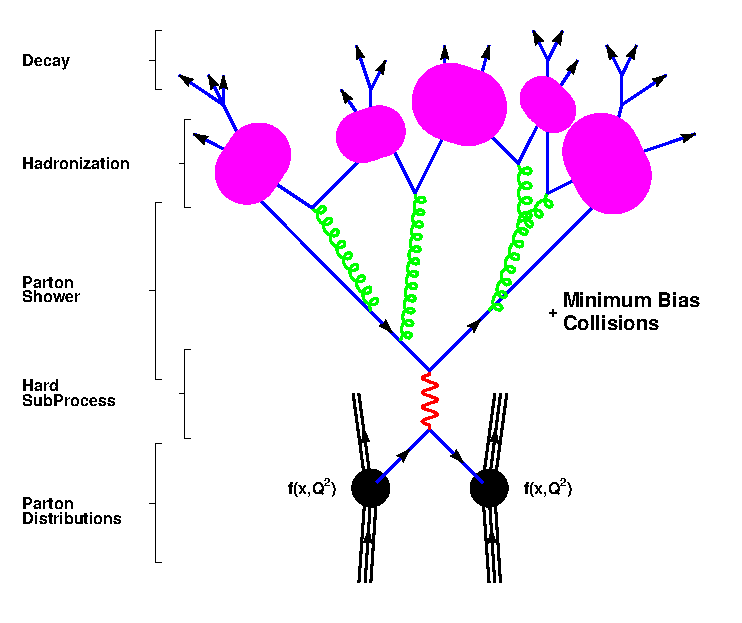
\includegraphics[width = 0.8 \textwidth]{Chapters/Chapter3/Figures/f_shg_event.eps}
 \caption{Schematical overview of the consecutive steps of the event generation process.}  \label{fig::EvtShower}
\end{figure}

\begin{myindentpar}
  \begin{description}
    \item[Parton Distribution Functions] \hfill \\
      In proton-proton collisions both incoming protons can be viewed as a collection of partons whose momentum fraction $x$ within the hadron is parametrized by the so-called parton distribution functions.
    \item[Hard scattering] \hfill \\
      Hard scattering is the perturbative process of two colliding partons, one originating from each proton, that creates high-energetic particles. It can be represented by a factorized product of short-and long-distance contributions as discussed in Section~\ref{sec::HardScattering}.
    \item[Parton shower] \hfill \\
      This phase of the event generation process describes the approximate higher-order corrections induced by emission of additional gluon and/or quarks, as will be explained in Section~\ref{sec::PS}. Depending whether this radiation originates from the incoming or outgoing partons it is denominated, respectively, Initial State Radiation (ISR) or Final State Radiation (FSR).
    \item[Hadronisation] \hfill \\
      The collection of \textit{(receding)} post-shower partons is combined into experimentally observable colour-neutral hadrons as required by colour confinement. This hadronisation process is described by QCD-inspired phenomenological models as discussed in Section~\ref{sec::Hadronisation}.
    %\item[Underlying event (why is this a separate item? Doesn't show up in the schematical overview ...)] \hfill \\
  \end{description}
\end{myindentpar}

The main challenge at hadron colliders \textit{(compared to lepton colliders)} is the missing information about the partons responsible for the hard interaction. 
The event generation process at the LHC is even more arduous due to the QCD activity in a widespread range of involved momentum transfer. %, according to the scale of momentum transfer involved. 
The interaction starts at a scale of barely $1$ $\GeV$ with partons confined in a proton beam, then produces during the hard interaction a few high-energetic outgoing leptons, gauge bosons or partons of which the latter afterwards transform non-perturbatively into final-state hadrons. This large variation in energy range, and corresponding QCD coupling strength, implies that only the high-momentum transfer part of the event generation can be derived exactly from the QCD Lagrangian while the other aspects have to be expressed using phenomenological non-perturbative models.

\subsection{Hard Scattering (=? Jet Fragmentation)} \label{sec::HardScattering}
Most events studied at the LHC involve high-momentum transfers in order to create massive particles or high-energetic jets. The inclusive production cross section of an observable $X$ from hadrons $h_1$ and $h_2$ for these type of interactions can be factorized into:

%Due to the internal structure of the protons, the inclusive cross section $\sigma_{h_{1}h_{2} \rightarrow X}$ cannot be calculated exactly from first principles but has to be factorized in terms of the partonic scattering cross section $\hat{\sigma}_{ab \rightarrow X}$ and the parton distribution functions $f_{a}^{h}$. Therefore, within the collinear limit~\cite{ColLimit}, the inclusive cross section for $X$-production can be written as:
%\\ \textit{Should check whether there is a difference between $\hat{\sigma}_{ab \rightarrow X}$ and $\hat{\sigma}(\Phi_{ab \rightarrow X},\mu^{2}_{F})$??}
\begin{equation} \label{eq::HSXS}
 \sigma_{h_{1}h_{2} \rightarrow X} =\sum_{a,b \in \{q,g\} } \int dx_{a} \int dx_{b} f_{a}^{h_{1}}(x_{a},\mu^{2}_{F}) f_{b}^{h_{2}}(x_{b},\mu^{2}_{F}) \int d\Phi_{ab \rightarrow X} \dfrac{d\hat{\sigma}(\Phi_{ab \rightarrow X},\mu^{2}_{F})}{d\Phi_{ab \rightarrow X}}
\end{equation}
From Equation~(\ref{eq::HSXS}) can be concluded that the hadronic cross section, valid for all orders in perturbation theory, is actually a convolution of a perturbatively short-distance component $\hat{\sigma}_{ab \rightarrow X}$, calculable from Matrix Elements, and an approximately long-distance one, represented by the parton distribution functions (PDF). The PDF $f_{a}^{h}(x_{a},\mu_{F})$ is the probability of encountering parton $a$ with momentum fraction $x_a$ in parent hadron $h$ when this is probed at energy scale $\mu_{F}$. This factorization scale $\mu_{F}$ symbolizes the transition from the short-distance process to the long-distance one (\textit{But this scale is motivated by the soft and collinear divergences which occur whenever a gluon is emitted from a quark so why already introduced in the hard interaction part ?}). 
The partonic scattering cross section $\hat{\sigma}(\Phi_{ab \rightarrow X},\mu^{2}_{F})$ depends on the final state phase space $\Phi_{ab \rightarrow X}$. 
\textit{\textbf{Does this last sentence really add something?}}\\

Equation~(\ref{eq::HSXS}) serves as the starting point for event simulation in general-purpose Monte Carlo event generators which, due to the perturbative nature of the parton-level differential cross section, can be expanded in orders of QCD coupling $\alpha_{S}$. Originally these calculations were performed at leading order (LO), corresponding to $\mathcal{O}(\alpha_{S}^{2})$, however this only describes the simplest processes taking place in hadron colliders and does not correspond to reality where additional radiation on top of $X$ occurs. Moreover the current theoretical precision for QCD requires at least next-to-leading order (NLO) calculations. Hence much effort has been devoted in order to overcome the infrared singularities in QCD allowing to extend the matrix element generators to perform these NLO calculations in an automated way and thereby (?) significantly improving accuracy and predictive power.\\

\textit{\textbf{Rewrite this part once is known which generators are actually used and which not at all ...\\}}
Many different event generators exist, but not all seem to be actually used for MC samples used in this thesis...\\
Herwig and Pythia are two general-purpose event generators, but they are both lacking NLO information. Only way to acquire NLO calculations is by incorporating full NLO corrections in the parton shower using the Powheg formalism. Sherpa is another event generator which has NLO information but does not seem to be used (so no need to discuss).\\
The more widely used event generators incorporate NLO corrections in the hard interaction: MadGraph/MadEvent, MC@NLO and Powheg.

\begin{myindentpar}
  \begin{description}
    \item[MadGraph/MadEvent] \hfill \\
      MadGraph is a matrix element generator for decays and $2$ $\rightarrow$ $n$ scatterings. \textit{(Not very clear, is it now NLO or is it tree-level ... ?)}
    \item[Powheg and MC@NLO] \hfill \\
      Powheg and MC@NLO are two event generators which are capable of calculating NLO corrections and, even more important, correctly matching them with the additional particles created during the parton shower step, which will be discussed in detail in \ref{sec::PS}
  \end{description}
\end{myindentpar}

\textit{What else can/should be written about this subject ...?}\\
\textit{Maybe brief discussion about LHAPDF and the used PDF set in this thesis (or does this only come after the Parton Shower part has been explained?)}

\subsection{Parton shower} \label{sec::PS}

The hard interaction does a great job in describing the primary collision between the two initial partons using the lowest order matrix-elements. However this process is lacking information about \textit{(the internal structure of jet and)} the non-perturbative confinement of partons into colour-neutral hadrons at low energy scales. This iterative process of higher-order emission corrections is defined by the Parton Shower (PS) formalism.

The partons formed during the hard scattering are prone to gluon radiation emission, $q$ $\rightarrow$ $qg$, and gluon branching, $g$ $\rightarrow$ $gg$. The first type of parton branching corresponds to Brehmstrahlung in QED while the second one has no analogy in QED and is caused/provoked by QCD's non-abelian nature. Both processes are incorporated in the PS formalism which sequentially lowers the transverse momentum of the contributing partons until the QCD confinement limit is reached, resulting in a broad parton cascade.
\\

The parton shower formalism's objective is to convert the inclusive cross section for the production of parton $a$ into the exclusive cross section taking into account a number of additional less-energetic particles.
%represent the large number of final state partons as a primary hard interaction surrounded with (chains of parton branchings) showers. 
Hence the complex $2$ $\rightarrow$ $n$ process will be decomposed into a hard interaction with momentum transfer $Q$ and a succession of gluon radiations each with momentum transfer $Q_{i}$; a justifiable approach in the approximation $Q_{i}^{2}$ $\ll$ $Q^2$ which is defined as the collinear\footnote{Two particles are collinear in case they are close in angle.} limit. 
%\textit{The exclusive cross section of the overall process can be associated with the cross section of the hard interaction but incorporates minor deviations to take into account the reduced energy available for the hard scattering due to the initial state radiation. \textbf{Really useful this XS info?}}
The Alterelli-Parisi splitting functions, denoted $P_{ba}(z)$, describe this collinear splitting of parton $b$ into parton $a$ and are defined as~\cite{}:
%The collinear splitting of parton $b$ into parton $a$ is described by the Alterelli-Parisi splitting functions $\hat{P}_{ba}(z)$, defined as~\cite{}:
\begin{eqnarray}
 & P_{qq}(z) = \dfrac{4}{3} \dfrac{1+z^{2}}{1-z}    & P_{qg}(z) = \dfrac{4}{3} \frac{1+(1-z)^{2}}{z} \\
 & P_{gq}(z) = \dfrac{n_{f}}{2} (z^{2} + (1-z)^{2}) & P_{gg}(z) = 3 \dfrac{z^{4}+1+(1-z)^{4}}{z(1-z)}
\end{eqnarray}
where $n_{f}$ represents the number of quark flavours.
\\
These splitting functions are divergent in the case of $z$ $\rightarrow$ $0$, corresponding to soft gluon emission as $z$ is the momentum fraction carried away by the parton $a$. 
Since reality is known to be finite these soft divergences, together with the collinear divergencies ($\theta$ $\rightarrow$ $0$), have to be excluded by introducing a cut-off scale on the transverse momentum $k_{t}$ ($\simeq$ $E\theta$ \textit{relevant?}) below which all remaining perturbative effects are absorbed by the parton distribution functions. 
The freedom of choosing this factorization scale $\mu_{F}$, generally around $1$ $\GeV$, necessitates the introduction of the DGLAP (Dokshitzer-Gribov-Lipatov-Altarelli-Parisi) evolution equations~\cite{}, which represent the fact that any parton $a$ may have been produced by the branching of parton $b$ at slightly higher scale $\mu_{F}^2 + d\mu_{F}^2$:\\
\begin{equation}\label{eq::PSProb_NoSudakov}
 \mu_{F}^2 \dfrac{d f_{a}^{h}(x,\mu_{F}^{2})}{d \mu_{F}^{2}} = \sum_{a \in \{q,g\} } \int_{x}^{1} \dfrac{dz}{z} \dfrac{\alpha_{S}}{2 \pi} \hat{P}_{ba}(z) f_{b}^{h}(x/z, \mu_{F}^{2})
\end{equation}

---------------------------------------------\\

The probability for a parton branching $b$ $\rightarrow$ $a$, represented by $\mathcal{P}_{ba}$, diverges in the limit of soft-gluon radiation
%, dependent on the numerator of the splitting function $z$ $\rightarrow$ $0$ and/or $z$ $\rightarrow$ $1$, 
and in the limit of collinear parton radiation, $Q^{2}$ $\rightarrow$ $0$.
%$z$ $\rightarrow$ $0$ and $Q^{2}$ $\rightarrow$ $0$, corresponding to soft gluon radiation and collinear parton radiation respectively. 
Both divergences are regulated by introducing a cut-off scale $Q_{0}$ for the parton shower iteration at about $1$ $\GeV$. In the occurence of soft-quark branching (\textit{Why is this still allowed, even after the cut-off is applied? (or is soft quark still larger than 1 GeV?})), the parton branching probability $\mathcal{P}_{ba}$ exceeds unity which would violate the total conservation of probability. This conservation is restored by including a Sudakov form factor, which represents the probability of a parton not to undergo a branching. Hence Equation~(\ref{eq::PSProb_NoSudakov}) has to be multiplied by this Sudakov factor and reformulated as:
\begin{equation}
 d\mathcal{P}_{ba} = \dfrac{\alpha_{S}}{2\pi} \dfrac{4}{3} \dfrac{dQ^{2}}{Q^{2}} P_{ba}(z)dz ~ \exp \left\lbrace - \int_{Q_{0}^{2}}^{Q^{2}} \dfrac{dQ^{'2}}{Q^{'2}} \dfrac{\alpha_{S}}{2\pi} \int dz^{'} P_{ba}(z^{'})  \right\rbrace
\end{equation}
%\\
%\textit{$P_{ba}$ can be easily translated to $P_{b \rightarrow a+c}$ by applying the allowed emissions.\\
%qq corresponds to q $\rightarrow$ q which can only be accompanied by gluon radiation hence $P_{qq}$ = $P_{q \rightarrow q g}$ in the definition used above. (check papers for rest)}\\
%\\
%\textit{Such higher order corrections occur in processes where a soft gluon is emitted or when a gluon or light quark splits into two almost collinear partons (NOT OWN WORDS)\\
%Only here does the Sudakov Form Factor and DGLAP equations enter the picture. So they describe the non-perturbative corrections to the hard interaction cross section caused by the soft and collinear splitting of the initial and final state partons.}

The parton shower algorithm outlined above is applicable for both initial and final state radiation since the branching probabilities are similar in both cases. However the actual implementation in the Monte Carlo event generators is performed in an entirely different way. This because each parton branching significantly reduces the energy of the initial partons and therefore the possibility to produce the hard process of interest, such as top-quark pair production. 
%In order to avoid the generation of billions of events and keeping only a couple relevant ones, the Monte Carlo event generators employ a backward method. 
Hence the Monte Carlo event generators employ a backward method, meaning that they start from the desired hard interaction and surround the initial partons with additional radiation (\textit{only}) afterwards.

\subsubsection{Combine hard scattering with parton showering}
\textit{Is this also relevant for LO calculations?}\\
\textit{Is only matching used or also merging? (Seems to be applied in HERWIG)}\\

\textit{At leading order correct matching between the produced jets and the original partons asked during the hard interaction is also important. This because additional hard gluon radiation in a X+parton interaction results in the same pattern as the hard interaction of a X+2-parton event. At LO there are two existing methods that can be used in order to avoid double counting: CKKW and MLM. The latter one, MLM named after M.L. Mangano, is the easier of the two and currently implemented in $ALPGEN$ for use with both $\Herwig$ and $\Pythia$.\\
At next-to-leading order the situation is a bit more complex and two different methods have been developed, $MC@NLO$ and $Powheg$. The former one has a wide range of processes available but can only be used in combination with $HERWIG$. However since recently, effort has been made to also combine the $MC@NLO$ approach with $\Pythia$ and $HERWIG++$. This in contrast to the latter one, which can be intertwined with both $HERWIG$ and $PYTHIA$ but is only recently catching up in the number of available processes.}\\

\textit{What should exactly be discussed?}
The current progress in calculating NLO hard cross section implies a profound understanding and description of the matching between the hard scattering and the parton shower. This is necessary in order to avoid double-counting.

%\subsubsection{Initial State Radiation (ISR)}
%The probability for the incoming partons in the parton bunch to radiate is similar to the branching probability of the partons produced by the hard scattering. Therefore exactly the same formulas and theory can be applied to the radiation of the inital-state partons. However there is an important difference between the initial-state radiation in reality and the implementation in the Monte Carlo event generators. This because the high branching probability significantly reduces the energy of the initial partons and hence the possibility to maintain sufficient energy to produce the hard process of interest, such as top-quark pair production. It would imply, as occurs in reality, the generation of billions of events in order to keep only a couple of thousand of interest. As a result, the Monte Carlo event generators actually start from the relevant hard process and work their way back to the initial partons to surround them with additional radiation.

\subsection{Hadronisation} \label{sec::Hadronisation}
The event generation algorithm designed up to now correctly describes the desired hard interaction and adequately surrounds it with soft-gluon radiation and parton production without any risk of double-counting. However one important aspect is still missing, namely the hadronization process, (\textit{comma issue with namely ...}) which describes how the quarks and gluons turn into experimentally observable colour-neutral hadrons.
This final step of the event generation cannot be calculated from first principles and is hence represented by phenomenological models.
Two distinct models for describing this non-perturbative process are used today, (\textit{Correct comma use?}) the Lund string model~\cite{Lund} and the cluster model~\cite{ClusterModel}, which are implemented in $\Pythia$ and $\Herwig$, respectively.

The former one is based on linear confinement, which states that the potential $V$ between a quark-antiquark increases with separation distance $r$ due to the presence of a strong QCD colour field.%, as depicted in Equation~(\ref{eq::VQCD}).
\begin{equation}\label{eq::VQCD}
 V = \kappa r ~~~ \kappa \sim 1 \dfrac{\GeV}{fm}
\end{equation}
Hence the kinetic energy of this parton pair will transform into potential energy as they move further away. If the energy stored within the colour string stretched between the quark $q$ and anti-quark $\bar{q}$ is large enough, it will split into a new $q\bar{q}$ pair with two distinct colour strings surrounding the parton pairs. The newly created particles have partly absorbed the potential energy of the original colour string and this process continues until the potential energy is too low for any additional string splittings to occur.
\\
This splitting, $(q\bar{q})$ $\rightarrow$ $(q\bar{q}^{'})$ + $(\bar{q}q^{'})$, is not known from first principles and is(, in this Lund string model,) explained by quantum mechanical tunneling phenomena. The probability for the creation of a quark with mass $m$ and transverse momentum $p_{T}$ during such a splitting is given by:
\begin{equation}
 \exp \left( -\frac{\pi m^{2}}{\kappa} \right) \exp \left(-\frac{\pi p_{T}^{2}}{\kappa} \right)
\end{equation}
The above formula only describes the formation of light $u$-, $d$- and $s$-mesons. Due to the presence of the quark-mass term, the production of heavier mesons is suppressed during this step of the event generation process. The string model also explains baryon-formation, this by allowing string breaks to produce diquarks according to the Lund symmetric fragmentation function:
\begin{equation}
 f(z) \propto \frac{1}{z} (1-z)^{a} \exp \left( - \frac{b(m_{h}^{2} + p_{T,h}^{2})}{z} \right)
\end{equation}
with $z$ the fraction of longitudinal momentum \textit{fraction of what???} carried by the hadron. For the creation of heavy $c$- and $b$-baryons an additional factor of $1/z^{bm_{Q}^{2}}$ has to be taken into account~\cite{} (\textit{Check reference 75 of paper QCD for collider physics}).

The second hadronisation model, the so-called cluster model, is based on the preconfinement property of QCD~\footnote{This implies that colour singlet combinations of partons (= clusters) can be formed with an asymptotically universal invariant mass distribution \textit{NOT OWN WORDS}}. At the end of the parton shower gluons are splitted into $q\bar{q}$ pairs and colour-connected pairs give rise to clusters from which hadrons are formed. \textit{More detail needed on this second model ?}

\textit{Something about decay of unstable particles?}

\subsection{Underlying event}% and Multiple Parton Interactions (?)}
Up to now only the ideal situation has been considered: the event generation process when only one parton present in the proton results in a hard interaction. However reality is a completely different story, and, since all the exchanged QCD particles carry colour charge, rather complex.\\
(\textit{Link sentences ...}) Two distinct soft phenomena contribute to the so-called underlying event (UE), the beam remnants and the multiple parton interactions (MPI). The beam remnant is defined as the remainder of the proton after the hard-interacting parton is knocked out. Originally the interacting proton was colour-neutral but the beam remnant ends up with a non-zero colour charge. Therefore it will start to hadronise and will influence the formation of hadrons during the hadronisation process. (\textit{Is this completely correct?}) The contribution of the multiple parton interactions can easily be understood by depicting the hadrons as a bunch of protons. Hence each of these protons is as likely to undergo scattering processes within one single hadron-hadron interaction\footnote{This can also result in hard scattering no? But if this happens the event will not be chosen and rejected?}.

As mentioned before, the exchanged QCD particles have colour charge implying that even a limited number of soft particles produced in this underlying event can have a major influence on the particle multiplicity in the final state. 
\textit{Mention something about the consequences ...}

In 1987, Sj\"ostrand and van Zijl proposed a first detailed Monte Carlo model for perturbative MPI, which is still considered as the basis for modern implementations~\cite{SjostrandAndZijl} (Check reference 76 of QCD for Collider Physics). \textit{Is this model-part necessary?}\\
\textit{Now something about implementation in Monte Carlo event generators maybe ?}\\

\textit{Should check whether UE is one of the important systematics or not... This determines in how much detail this section should be explained!}

\section{Simulating detector response} \label{sec::DetectorSim} %Detector simulation (CHANGE TITLE!)}

\section{Physics object reconstruction (CHANGE TITLE!)} \label{sec::PhysicsObjects}

\textit{Important to first explain the separate construction of both the muon and electron candidates because they are actually used as a starting point for the PF algorithm. The PF algorithm should not be seen as something completely disconnected because was actually added on top of the already existing reconstruction methods in order to improve the efficiency and reduce the corresponding fake rates.}

\subsection{Muon reconstruction}\label{subsec::Muon}

The muon reconstruction algorithm is designed such to fully exploint the excellent reconstruction efficiency in both the tracker and the muon system.
%Since the muon traverses the entire tracker detector without siginificant energy loss it will produce detectable hits in multiple layers of the tracking system. 
Hence tracks reconstructed in the inner tracker and the muon system separately are combined into actual muon candidates. In order to distinguish these two types of muon-seeds they are called \textit{tracker track} and \textit{standalone-muon track}, respectively.

The identification of standalone-muon tracks is performed in two consecutive steps. First local reconstruction \textit{starts by (?)} constructing track segments from the detected hits in the DT and/or CSC chambers. Afterwards the track segments found in the innermost chambers are used as seeds for the standard reconstruction algorithm based on the Kalman Filter technique, as discussed in Section \ref{sec::KFTracking}. First an inside-out Kalman Filter is applied which\footnote{ (takes into account the muon energy loss in the material, the effect of multiple scattering and the non-uniform magnetic field. -- or is this general the case for a KF?) This procedure} propagates the muon track to the next layer, compares with the measured energy deposits and updates the track parameters accordingly. Once the most outer layer of the muon system is reached, an outside-in Kalman Filter is performed which calculates the track parameters at the most inner muon station. Finally, in order to improve the momentum resolution, an additional beamspot constraint is applied to the track parameters before the actual standalone-muon track is identified.

Actual muon candidates combining information from both the tracker detector and muon system can be obtained using two separate methods. In case the muon identification starts from the standalone-muon tracks so-called \textit{global muons} are reconstructed while the collection of tracker tracks gives rise to \textit{tracker muons}.
%Depending on whether the the muon candidate is reconstructed starting from the standalone-muon tracks or from the tracker tracks, it is defined as a \textit{global muon} or a \textit{tracker muon}, respectively. 
The global muon candidates are reconstructed by identifying a matching tracker track, for each standalone-muon track, by propagating both track parameters onto a common surface. Then for each pair the hits of both tracks are used to fit a global-muon track using an outside-in Kalman Filter Technique. The identificitation of muon candidates as global muons is especially powerful when a high quality muon track was found in the muon detector. However in some cases it can occur that the standalone-muon reconstruction fails because of a lack of hits. This is most likely to happen in the presence of low transverse momentum muons which are not able to deposit sufficient energy deposits in the muon spectrometer. Hence for these type of muons the tracker-muon reconstruction is very useful since it extrapolates all tracker tracks with transverse momentum $p_T$ $>$ $0.5$ $\GeV$ and total momentum $p$ $>$ $2.5$ $\GeV$ to the muon system. If at least one muon segment matches this extrapolated track, the tracker track fullfilled the tracker muon requirements and is identified as such.
%The first collection is created by matching a tracker track for each standalone-muon track using again an outside-in Kalman Filter technique to combine the track parameters.
%The second collection follows an inside-out approach and extrapolates all tracker tracks with transverse momentum $p_{T}$ $>$ 0.5 GeV and total momentum $p$ $>$ 2.5 GeV to the muon system.

Since both approaches have specific benefits, tracker muon reconstruction is more efficient for low momentum muons while global muon reconstruction is efficient for high energetic muons which traverse multiple muon segments, they are combined in order to have a robust and highly efficient (\textbf{How much?}) muon reconstruction (\textit{throughout all energy ranges}). \textit{\textbf{Useful? -- Best to mention this after the two types of muons are explained or is within the text above also helpful?}}
\\

\textit{Something about charge identification necessary?}
%\textit{Difference between Global Muons and Tracker muons explained in ``Performance of CMS muon reconstruction in pp collision events at 7 TeV''. Both of them are used as basis for the PF algorithm, and hence can be considered as the ``reco muon'' collection in ``Commissioning of the PF event reconstruction with leptons from J/Psi and W decays at 7 TeV''.}
%
%In order to take advantage of the high momentum-resolution in the silicon tracker for low-momentum muons the obtained standalone muon is compared with corresponding tracks reconstructed in the tracker.
%A Kalman-filter based track fit, which uses information from all hits in both the tracker track and the muon track, is performed. The considered standalone muon, combined with its best-matching tracker track, is then promoted to a so-called global muon. 
 
\subsection{Electron reconstruction} \label{subsec::Electron}

Due to the thickness of the CMS tracker a dedicated elektron-track reconstruction is necessary in order to correctly account for the energy loss caused by Brehmsstrahlung. 
This photon radiation significantly lowers the initial momentum of the electron and spreads it out, mainly along the $\phi$ direction resulting in a more complex and less straightforward electron reconstruction algorithm.
In stead of the general Kalman Filter track reconstruction approach, explained in Section \ref{sec::KFTracking}, the electron-reconstruction algorithm is based on a Gausian Sum Filter (GSF) fit, which allows to model changes in curvature radius throughout the different tracker layers. Because this GSF fit is rather CPU intensive it is only applied on a subset of track seeds defined electron seeds.
%The downside of this GSF fit is that it is rather CPU intensive and can therefore only be applied on a subset of track seeds.

%Since the electrons traverse a (vast) amount of matter before reaching the electromagnetic calorimeter where they can deposit their energy, Brehmsstrahlung will occur. 
%As a consequence the electron reconstruction algorithm is more complex and less straightforward than the previously discussed muon reconstruction algorithm.%, however, the main idea still comes down to associating a charged-particle track with an ECAL cluster.

In order to identify the subset of electron seeds relevant for the electron-track reconstruction, two different seeding algorithms can be considered: ECAL-based or tracker-based.
The ECAL-based approach starts from the energy deposits recovered in the electromagnetic calorimeter and extrapolates then back to the interaction vertex. In order to take into account the Brehmsstrahlung effects, the cluster is enlarged into a so-called supercluster and the extrapolation to the tracker is performed from the energy-weighted average position of this supercluster. The tracker seeds compatible with the hits obtained from this supercluster extrapolation are then defined as electron seeds. The tracker-based approach starts from charged-particle tracks reconstructed with the general KF reconstruction algorithm. The corresponding tracker seeds are then obtained using a MVA method in order to only select the ones compatible with the electron-particle hypothesis.
%\textit{Need to mention that only a subset of tracker seeds, obtained using either an ECAL-based or either a tracker-based seeding algorithm, are given as input to the GSF track fitting algorithm.}

After the identification of the relevant tracker seeds, the electron-track fitting can be performed. As mentioned above, this is done by a Gaussian Sum Filter fit which represents the energy loss in each tracker layer by a mixture of Gaussian distributions. This approach is more correct in the presence of Brehmsstrahlung because the standard Kalman Filter fit only assumes a single Gaussian energy loss distribution for a particle traversing the detector. The track fitting provides electron-tracks up to the electromagnetic calorimeter such that the corresponding track parameters can be obtained at the ECAL surface. Hence the energy fraction lost by the electron due to Brehmsstrahlung can be estimated.

%\textit{The starting point of the electron reconstruction algorithm is similar to the one of the muons, namely tracker seeds. However, in contrast with the muon case, the electron candidate tracker seeds cannot be converted into actual electron tracks using the standard Kalman Filter approach discussed in Section \ref{sec::KFTracking}. This because this standard approach assumes that the energy loss distribution of the considered particle going through the detector is represented by a Gaussian, a good approximation in absence of Brehmsstrahlung. Hence the track fitting for electrons is done by a Gaussian Sum Filter (GSF) which represents the energy loss in each tracker layer by a mixture of Gaussian distributions.}

%At first the electron energy deposited in the electromagnetic calorimeter is combined into so-called superclusters, which collect the energy in a small window in $\eta$ and an extended window in $\phi$ in order to take into account the Brehmsstrahlung deposits.
%\\
The GSF tracks recovered with the above mentioned reconstruction algorithm can then be translated into actual electron candidates in two different ways. Either by a track-cluster association criterion or otherwise by the PF event reconstruction algorithm. The former one, which depens on the seeding method used, will be discussed here while the PF-approach will be discussed in Section \ref{subsec::PF}.
In case of the ECAL-based seeding algorithm the electron track is simply associated with the supercluster which was used to reconstruct the corresponding tracker seed using a geometrical matching. For the tracker-based seeding algorithm the association is made with a PF cluster based on a MVA combining information on track observables and electron PF cluster observables. \textit{So how is dealt with the photon ECAL deposits in this case?} 
%\textit{Is the PF electron approach really complete separate from the one explained here? Doesn't seem to be the case since it combines bits and pieces of this general reconstruction algorithm.}

\subsection{The Particle-Flow event reconstruction algorithm} \label{subsec::PF}

In order to optimally reconstruct the direction, energy and type of all stable particles the particle-flow (PF) algorithm combines the information of the different CMS subdetectors. The obtained collection of individual particles is then used to reconstruct jets and determine missing transverse energy.
The main benefit of the PF approach is the large efficiency gain by combining less precise subdetectors with more granular ones.

The PF algorithm uses a stepwize approach \cite{}, starting by identifying fundamental elements such as charged-particle tracks, calorimeter clusters and muon tracks. Then the algorithm links these distinct building bricks of the different subdetectors topologically in order to form so-called building blocks. As a final step the blocks are converted into stable particles.
%(\textit{This approach exploits the high granularity of the ECAL and the very precise tracker immersed in a uniform axial magnetic field of 3.8 T.})

\subsubsection*{Reconstructing and combining the fundamental elements}

Since most stable particles have rather low momenta, even in very energetic collisions, the building bricks used by the PF event reconstruction algorithm have to be measured with very high efficiency and a low fake rate. 

The iterative tracking algorithm used to reconstruct charged-particle tracks fullfills (both) these requirements with flying colours. The CMS tracking detector can be considered the cornerstone of the PF event reconstruction since it measures the momentum of charged hadrons with a higher resolution than the calorimeters and provides furthermore a precise determination of the charged-particle direction at the production vertex before any influence from the magnetic field. The iterative tracking algorithm starts from very tight charged-particle seeds and progressively loosens the track seeding criteria. At each iteration hits assigned to the tracks found during the previous iteration are removed (\textit{What is this part doing?})

The calorimeter clusters are reconstructed in a high efficient and low fake rate manner using a clustering algorithm specifically developed for the PF event reconstruction. In this algorithm the seeds are defined as calorimeter cells with energy above a certain threshold. These cluster seeds are then transformed into so-called topological clusters by accumulating calorimeter cells adjacent to the cells present in the cluster. In order to suppress electronics noise the calorimeter cells are required to exceed a given energy threshold. Finally each topological cluster results in multiple particle-flow clusters, as much as cluster seeds present in the topological cluster.

Since each particle is expected to give rise to various building bricks a non ambiguous linking algorithm that excludes any possible double-counting is applied. This algorithm connects elements presumed to correspond to the same particle and quantifies the quality of the linkage by the distance between the considered elements. For example a charged-particle track is linked with a PF calorimeter cluster if its extrapolated position lies within the cluster boundaries. This specific linking is also performed between charged-particle tracks and ECAL clusters in order to take into account the energy deposited by Bremsstrahlung photons emitted by electrons. Because the above explained clustering algorithm is performed separately in each of the calorimeter sub-detectors linking between different calorimeter clusters is also considered. In this case a linkage is established when the cluster position of the more granular calorimeter is within the cluster envelope of the less granular one. Finally the linking algorithm matches charged-particle tracks and muon tracks based on a global $\chi^{2}$ track fit in order to create so-called global muons. \textit{Is this really part of the PF algorithm, this is the Global Muon reconstruction ...}

\subsubsection*{Identifying stable particles}
After establishing the fundamental elements and the linkages amongst them, the list of reconstructed particles is (identified) by the particle-flow algorithm. This happens gradually by first identifying the PF muons and PF electrons while the remaining elements will give rise to charged hadrons, photons or neutral hadrons.

The collection of Global and Tracker muons, explained in Section \ref{subsec::Muon}, contain significant contamination from misidentified charged hadrons. In order to promote these muon candidates to PF muons they have to be distinghuised from charged hadrons by the PF algorithm. This is done using three separate selections: isolated, PF-tight and PF-loose. The isolated selection is applied first, considers only global muons and has the loosest selection of all three (\textit{since almost no additional neutral particles are expected to lie within their vicinity}). The remaining muon candidates are passed to the PF-loose and PF-tight selection, which are developed such to identify muons within jets. The PF-tight selection aims to reject \textbf{hadronic punch-through\footnote{Defined as hadron shower remnants penetrating through the calorimeters and reaching the muon system.} (?)} by combining information from the muon system and the calorimeters while the PF-loose selection tries to recover muon candidates that have a track momentum significantly larger than the corresponding calorimeter deposit, a combination incompatible with the charged hadron hypothesis.

Next the PF algorithm reconstructs electrons starting from the GSF track, discussed in Section \ref{subsec::Electron}. Because of possible curvature alteration caused by Brehmsstrahlung the outermost track layer position of the GSF track is extrapolated to the ECAL and associated with the closest PF cluster. Afterwards the energy of the corresponding identified Brehmsstrahlung photon clusters are assigned to the total electron energy. Finally the electron candidates are distinghuised from charged hadrons using a multivariate analysis based on variables related to energy and geometrical matching between the track and the cluster, two purely calorimeter-based variables and several genuine tracking quantities.

%\textit{Should find another reference, current paper doesn't give the same explanation as in thesis Stijn ...}\\
%\textit{Simple summary seems to suggest that a charged hadron is recovered in case of a linked particle track with a cluster is encountered. After the removal of these charged hadrons the only remaining particles are neutral hadrons and photons. }\\
After the identification of the PF muon and PF electron candidates the remaining charged-particles tracks and PF calorimter clusters are translated into charged hadrons, photons or neutral hadrons.
Whenever a particle track linked with a calorimeter cluster that has compatible energy measurements it is defined as a charged hadron candidate. In case the calorimeter measurement is larger the excess is assigned to a photon or a neutral hadron. The former ones are identified as a cluster in the ECAL while the latter ones correspond to a cluster in the ECAL. The remaining calorimeter clusters which are unmatched with a charged particle track are also assigned to photons and neutral hadrons. \textit{extensive enough?}

\subsection{Jet reconstruction}
 \textit{Check ``Commissioning of the PF event reconstruction with the first LHC collisions recorded in the CMS detector'' section 6!}\\
 $\rightarrow$ Is rather limited on jets ...\\
 
The reconstruction of jets is less straightforward than the other physics objects explained before because they should be seen as a collection of hadronic activity combined into a single cone. However the event topology of interest, $t\bar{t}$ $\rightarrow$ $bjjbl\nu_{l}$, contains four jets so reconstructing this object in a correct and accurate way is very important.
 
\subsubsection*{Jet clustering algorithm}
Many different jet clustering algorithms exist but in this thesis only the cluster-based ones will be explained in detail. This type of jet clustering algorithms starts from a collection of stable partons and calorimeter cells and combines them into a cone with radius $R$ \textit{(Is this really correct? --  can also use 'into a jet')}. This clustering procedure uses a distance-based approach since it looks for each object $i$ whether another object $j$ can be found within the predefined cone radius $R$ taking into account the transverse momentum $k_{\bot}$ of both objects.

The distance measures used in this jet clustering algorithm are given in Equations (\ref{eq::JetClustering1}) and (\ref{eq::JetClustering2}) where the first one defines the distance between the two objects while the second one represents the distance between the object $i$ and the beam (B). Here $\Delta_{ij}^{2}$ $=$ $(y_i - y_j)^{2} + (\phi_i - \phi_j)^2$, the $(y,\phi)$ distance between both objects and $p$ can be intepreted as a parameter which controls the relative power between the energy and the geometrical scales.
\begin{eqnarray}
 d_{ij} & = & \min(k_{\bot i}^{2p}, k_{\bot j}^{2p}) \frac{\Delta_{ij}^{2}}{R^{2}} \label{eq::JetClustering1} \\
 d_{iB} & = & k_{\bot i}^{2p}                                                      \label{eq::JetClustering2}
\end{eqnarray}

The jet clustering algorithm now creates jets by looking for the smallest of these distances. Whenever the distance $d_{ij}$ is smallest, the objects $i$ and $j$ are merged into a single object and stored as such in the list. However, in case the distance $d_{iB}$ is smallest, the object $i$ is removed from the list of input objects and categorized as a final jet. Afterwards the distances are recalculated and this procedure continues until no input objects remain.

The merging of two different objects into a single one is done using one of the existing recombination scheme, in the case of this thesis the E recombination scheme is used. This scheme calculates the four-momentum of the new object by simply adding the four-momentum of its constituents. (\textit{What about eta and phi?? -- explanation about ET scheme needed as well?})

The value given to the parameter $p$ defined in the two distance definitions, which governs the relative power of $k_{\bot}$ versus $\Delta_{ij}^{2}$, results in different cluster-based jet algorithms; two of which are used in this thesis. When this parameter takes the value $1$ the $k_{\bot}$ algorithm can be retrieved, which is used in ... . 

In the case of $p$ $=$ $-1$ the jet algorithm is defined as the anti-$k_{\bot}$ algorithm. This algorithm is used for ... (\textit{\textcolor{red}{How to know where which algorithm is used??}})
Within this jet clustering algorithm soft particles prefer/tend to cluster with hard particles (in stead of with other soft particles) implying robust jet boundaries with respect to soft radiation. Both jet clustering algorithms are infrared and collinear safe, meaning that the created jet collection is not sensitive to soft emission and collinear splitting, respectively.

\subsubsection*{Jet Energy Scale corrections}
\textit{Also so much detail needed as in case of Stijn? Or only if this is an important systematic?}

Will need to explain here that the ``raw jet energies are corrected to obtain a uniform response in $\eta$ and an absolute calibration in $p_T$''. (See arXiv 1107.4277)

\subsubsection*{Jet energy resolutions}

\subsubsection*{Identification of b-quark jets}

B-jet identification \textit{consists} of building observables which can be used to exploit the differences between b-quark and light flavoured jets. These algorithms, many exist in literature, allow to distinghuish the event topology of interest from the large bulk of background events which only contain light-parton jets.
The different b-jet identification or b-tagging algorithms rely on the reconstructed objects defined above altough some minor optimization requirements are implied in the case of track selection. (in order to improve the b-tagging efficiency).

One of the main b-quark jet characteristics which is exploited by the b-tagging algorithms is its relatively long lifetime resulting in the presence of a displaced vertex with respect to the interaction point. Since only the tracking detectors offer the spatial resolution needed to detect the displacement between the primary and secondary vertices, they are reconstructed purely from the track collection. In order to be able to cope with multiple proton-proton interactions the tracks are required to be within a cone of $\Delta R$ $=$ $0.3$ around the jet axis, defined by the direction of the jet momentum. 
The actual reconstruction of secondary vertices is an iterative process using an adaptive vertex fit. This fit algorithm estimates the position of the vertex candidate and removes all its associated tracks from the track collection. This fit procedure is repeated until no new vertex candidates can be found. During the first iteration the interaction point is used as a constraint in order to identify the prompt\footnote{Prompt tracks are tracks originating near the pp interaction point!} tracks.

The different b-tagging algorithms which exist can be divided into two distinct categories; one which distinghuishes b-quark jets from light jets based on the track impact parameters and another based on the secondary vertices. Within this thesis only the second type of b-tagging will be utilized, namely the \textit{Combined Secondary Vertex} (CSV) algorithm. This algorithm combines the secondary vertex information together with the track-based lifetime properties (\textit{What are these?}). Because both characteristics are combined the algorithm is also capable of discriminating between both types of jets in cases where no secondary vertex was found but where reduced track constraints give rise to a pseudo-vertex and even in cases were no vertex could be reconstructed.

The b-tagging algorithms are constructed in such a way that they should only be applied for three predefined operating points which correspond to a specific misidentification probability for light partons of roughly $10 \%$, $1 \%$ and $0.1 \%$ for an average jet $p_T$ of about $80$ $\GeV$ defined respectively as \textit{Loose}, \textit{Medium} and \textit{Tight}. In this analysis only the Tight operating point is considered (\textit{\textcolor{red}{Where do you find these percentages??}})

%\subsubsection*{Old b-tagging}
%The specific characteristics of b-quark jets; long lifetime, large mass, decay to final states with high charged track multiplicities, $\cdots$; can be exploited in order to distinguish event topologies which produce $b$ jets in the final state from background events only containing light flavoured jets.

%Multiple different b-jet identification (b-tagging) algorithms exist which exploit different specific b-quark properties. Within this thesis only the b-tagging algorithm based on the information of the secondary vertices together with the track-based lifetime information, defined as the \textit{Combined Secondary Vertex} (CSV) algorithm, is used.
%Because each of the b-tagging algorithms requires a collection of well-reconstructed tracks of high purity some additional requirements are imposed on this sample of tracks. Also the reconstruction of the secondary vertices, vertices displaced with respect to the primary vertex, has an optimized track selection, this time because of the additional combinatorial reconstruction complexity in the presence of multiple proton-proton interactions. Hence tracks are required to lie within a cone of $\Delta R$ $=$ $0.3$ around the jet axis, defined by the direction of the jet momentum.

%The collection of secondary vertices is than constructed starting from this sample of optimized tracks and continues iteratively. A vertex candidate is identified by applying an adaptive vertex fit which assigns a weight based on the track's compatibility with the vertex position. All tracks with weight $>$ $0.5$ are removed from the list and the fit procedure is repeated until no new vertex candidates can be found. The motivation for applying an iterative fit algorithm is because the first iteration is mainly used for identifying the prompt tracks in the jet while the following ones produce decay vertex candidates. \textit{\textbf{So what does this actually mean??}}

%\textit{So what is actually the point, are tracks matched to the collection of secondary vertices or is something else done??}

\subsection{Missing transverse energy}
%\chapter{Recovering signal event topology} \label{chp:labelTitle}

The previous chapter described in detail how the individual physics objects can be identified and reconstructed.
However, due to the enormeous amount of proton-proton collisions produced at the LHC and collected by the CMS experiment, the main challenge of any physics analysis is achieving a succesful combination of identifying the relevant physics objects and ensuring the separation of the event topology of interest from the large bulk of background events.
This can be realized by developing an elaborate event selection procedure that excludes events based on specific kinematic requirements in a sequential manner, as will be discussed here.
\\
\\
Such an event selection follows a logical order and  \\
This event selection process generally starts from 
%\\
%\\
%In the previous section it was thoroughly described how the different physics objects can be identified and reconstructed.
%However, in order to study a specific type of interactions, semi-leptonically decaying top-quark events in this thesis, special attention should be devoted in order to select exactly these event topologies.
%This ... occurs in a sequential manner, starting from the general and centrally managed trigger system which aims to only store the events matching some predefined requirements and ranges up to an analysis-specific event optimisation to discard particular event signatures.
%\\
%\\
%This multi-layered event selection procedure will be explained in detail here, first focusing in Section~\ref{sec::MainSelec} on the more general steps such as triggering and cleaning of the relevant events together with the main selection criteria.
%Afterwards the additional selection constraints applied in order to single out the specific characterisations of this analysis will be discussed in Section~\ref{sec::SpecificSelec}.

\section{Selecting (clean) $\ttbar$+$\mu$ event topologies}\label{sec::MainSelec}
An important part of any physics analysis consists of selecting the event topologies compatible with the considered decay process and avoiding similar signatures by noisy events mimicking the requested final state particles. Hence a dedicated selection and cleaning procedure should be applied in order to remain with only the expected event topology. This is in general achieved by combining the online trigger system with a dedicated offline event selection (as will be discussed below).

\subsection{Triggering and cleaning of events}\label{subsec::Trigger}
As was already briefly mentioned in Chapter~\ref{chp:CERN}, CMS possesses a complex trigger system consisting of two levels in order to first perform a fast online decision to decide whether the event is deemed interesting enough to be calculated in more detail and eventually stored.
This trigger system contains an exhaustive list of slightly distinct trigger paths which all aim to identify a specific type of final state particles and rejecting the events not corresponding with the desired event topology, hence drastically reducing the stored event rate.

The final state signature expected for semi-leptonically decaying $\ttbar$ events can be distinghuished from the enormeous background in a rather straightforward manner by simply requiring the presence of a well-isolated lepton.
Hence the applied trigger asks for at least one isolated muon with the specific kinematic requirements of $\pT$ $>$ 24 $\GeV$ and $\vert \eta \vert$ $<$ 2.4 to be fullfilled.
\\
\textit{Is the cleaning part of the triggering? Or is this a separate thing which has to be applied by hand?}

\subsection{Lepton selection criteria}
Even though the chosen trigger path has restricted the lepton kinematics, the analysis-specific lepton selection should still be applied in order to further exclude unwanted events.
This because a trigger path is kept as general as possible such that it can be applied by various analyses.
The considered trigger for example is not specific enough for semi-leptonic $\ttbar$ events, which contain exactly one lepton originating from one of the W-bosons.
Therefore the offline selection criteria applied afterwards rejects events that contain more than one isolated muon for which the kinematic constraints are rather similar with the ones applied in the trigger: $\pT$ $>$ 26 $\GeV$ and $\vert \eta \vert$ $<$ 2.1. 

The next step in the event selection procedure focusses less on the kinematic information but aims to determine whether the considered lepton can be identified as a well-reconstructed one. 
In the case of the muon channel, these so-called muon identification criteria start from Particle-Flow muons, as discussed in Section~\ref{subsec::PF}, are responsible to suppress hadronic punch-throughs, cosmic muons and muons from decays in flight of other particles.
Therefore it is required that the candidate muon is reconstructed as a global muon for which the global-muon track fit, with normalised $\chi^{2}$ $<$ 10, should at least contain one muon chamber hit. 
Moreover the muon track should have at least two muon stations with matched segments, contain at least one pixel hit and more than five tracker layers with hits. The latter requirement will guarantee, besides suppressing muons from decays in flight, a good $\pT$ measurement for the muon.
Finally the muon candidate should originate from the primary vertex, which can be ensured by limiting both the longitudinal and transverse impact parameters ($\vert d_0 \vert$ $<$ 0.2 and $\vert \Delta z \vert$ $<$ 0.5).

Another important identification variable is the isolation which allows to distinghuish prompt muons with high purity from the ones embedded in jets since it determines the hadronic (what about photon) activity around the muon candidate at the interaction vertex. %in a cone of radius $\Delta R$ = 0.4 around the muon candidate. 
The isolation variable is defined as the scalar sum of the transverse energy of all the reconstructed particles contained within a cone of radius $\Delta R$ = 0.4, excluding the contribution of the muon itself.
\\
However the large number of additional proton-proton interactions complicates the identification of the interaction vertex such that a correction variable should be applied to ensure correct treatment of these supplementary interactions. Hence for the charged hadrons (CH) only the ones associated with the primary vertex are included in the scalar sum and for the neutral ones (NH and $\gamma$) a correction is applied which substracts the estimated PU contribution. This can be calculated by halving the PU contribution for charged particles since jets contain on average twice more charged PF particles than neutral ones~\cite{CHContrVsN}.
The $\Delta \beta$-corrected definition for the isolation variable is given in Equation (\ref{eq::DeltaBetaIso}) and is required to be fullfill $I_{\textrm{rel}}^{\Delta \beta}$ $<$ 0.12.
\begin{equation}\label{eq::DeltaBetaIso}
 I_{\textrm{rel}}^{\Delta \beta} = \frac{1}{\pT^{\mu}} \left( \sum_{\textrm{CH}} \pT^{\textrm{CH}} + \max(0, \sum_{\textrm{NH}} \pT^{NH} + \sum_{\gamma} \pT^{\gamma} - 0.5 \sum_{PU} \pT^{PU}) \right)
\end{equation}
\textit{Is it pT or ET?}\\
\textit{Need plots?}

\subsection{Jet selection criteria}
An notable difference in contrast to the leptons discussed before is that the PF jets require a few calibrations in order to correct for the small discrepancies observed between data and simulation (see \ref{subsec::jetReco}). These corrections need to be applied prior to the event selection for all jets \textbf{accounted for} in the event with $\pT$ $>$ 10 $\GeV$: charged hadron subtraction (CHS) which removes all the contributions of charged pileup, energy calibration using the L1L2L3 corrections and energy smearing in simulated events.
\\

Since the chosen trigger path does not restrict in any way the jets present in the considered event implies that the entire selection and cleaning process is taken care of by the offline jet identification criteria (\textit{Not even a minimum requirement on the pt?})
The actual event selection applied in this analysis requires an event to contain at least four high energetic jets ($\pT$ $>$ 30 $\GeV$) located within $\vert \eta \vert$ $<$ 2.4, which all have to be well separated from the identified lepton ($\Delta R$ $>$ 0.3).
The actual jet identification criteria have as goal to reject fake, badly reconstructed and noisy jets while still remaining with a pure sample of real jets and restrict the energy fractions of the different jet constituents. These criteria constrain the energy fraction of the charged electromagnetic PF particles ($f_{CEM}$ $<$ 0.99), the energy fraction of the charged PF hadrons ($f_{CH}$ $>$ 0), the energy fraction of the neutral electromagnetic PF particles ($f_{NEM}$ $<$ 0.99) and the energy fraction of the neutral PF hadrons ($f_{NH}$ $<$ 0.99).
\\

\textit{What about number of constituents and muon fraction ?? (+ what is this fHPD (0.98) and n90Hits in event selection file?)}

%\subsection{Data-MC agreement/Kinematics of selected events}
%\textit{Does not really make that much sense to show here the MSPlots since they do not agree at all ...}

\section{Fine-tuning of the event selection}\label{sec::SpecificSelec}

The event selection constraints discussed in the previous section are kept as general as possible in order to be applicable for numerous analyses examining a similar event topology.
Since these selection criteria are centrally managed, their performance is continiously monitored and changing detector conditions are easily taken into account.
In addition, the various synchronization exercises between the different analyses using the same selection criteria significantly improves the selection efficiency. (\textbf{Be sure this is the case!})
\\

The above-mentioned selection criteria, however, still have to be fine-tuned in order to incorporate the analysis-specific requirements.
The analysis discussed in this thesis actually requires a very stringent event selection mainly motivated by the choice to use a Matrix Element method, see Chapter~\ref{ch::MW}, to measure the anomalous couplings in the Wtb interaction vertex. Such a method examines an event using the full kinematic information and thus necessitates a large processing time for each event. As a result it has been decided to restrict the considered event sample as much as possible in order to avoid wasting computational resources on incorrect event topologies.
\\
\\
Two important background-reduction constraints have been applied, each focussing on a different kinematic property and thus aiming to exclude distinct types of events. 
The first one, which is discussed in Section~\ref{subsec::BTag}, exploits the characteristic signature of semi-leptonically decaying top-quark pair events: the expected presence of two jets originating from the decay of a b-quark. The second requirement, Section~\ref{subsec::MassCuts} focuses more on the kinematic properties of the reconstructed jets by demanding their mass combinations to correspond with the top-quark and W-boson mass.
To finalize, Section~\ref{subsec::DataMC} will give an overview of the applied event selection and will demonstrate some of the kinematic properties of the remaining event sample.
%An overview of the applied event selection and the kinematic properties of the remaining event sample will be discussed in Section~\ref{subsec::DataMC}.

%Up to now only general event selection constraints have been discussed, which are in general managed centrally and thus applicable numerous analyses. The different values of these kinematic constraints and identification criteria have been studied in great detail and are optimised in order to ensure the selection of a relatively pure sample of events.
%\\
%This however does not take into account the specific demands of the analysis discussed in this thesis where the followed procedure requires a small event sample. 
%This choice is motivated by the large processing time needed to process an individual event, such that it is beneficial to not waste resources on uncomplete events.
%As a result a couple of supplementary event selection requirements will be discussed in this section, with the largest background reduction one being the b-jet identification. The other selection constraints are smaller and focus purely on optimising the signal versus background ratio for the selected event sample.

\subsection{Background reduction using b-jet identification}\label{subsec::BTag}

Top-quark pair-production events for which one of the W-bosons decays hadronically and the other one leptonically are not merely characterised by the presence of a muon but also by the presence of two jets originating from the decay of the b-quarks.
Exploiting this latter property is an effective manner of distinguishing the event topology from the background, since the decay of the b-quarks has the peculiar feature that it gives rise to a displaced vertex. This is due to the relatively long lifetime of the b-quark such that the decay does not occur at the interaction vertex, as has previously been discussed in Section~\ref{subsec::jetReco}.
\\ 

For this analysis the b-jet identification is a crucial asset in reducing the background contribution since there has been opted for only selecting events for which at least two jets survive the b-tagging requirement. Since the main background samples for semi-leptonically decaying top-quark events might have events with one jet fullfilling this condition, the probability of having two such jets is significantly smaller (\textbf{Possible to give percentages?}). Hence the considered background samples; W-boson production in association with jets (W+jets), Z-boson production in association with jets (Z+jets) and single-top production in the t-, tW- and s-channel; will almost completely vanish/dissapear. (\textit{Check if this is also in someway the case when only a double light is applied! .. Yes, main background of W+jets is only 10 $\%$ of ttbar sample! (Total is 20$\%$ of ttbar)})
\\

The b-jet identification algorithms developed by the CMS collaboration are advised to only be deployed at specific working points defined as \textit{Loose}, \textit{Medium} and \textit{Tight}.
These correspond to a predefined tagging and misidentification probability of around 85$\%$, 69$\%$ and 52$\%$ and a mistagging efficiency of 19$\%$, 5$\%$ and 1$\%$, respectively, for the Combined Secondary Vertex (CSV) b-tagging algorithm. (\textit{Good to repeat again ?})\\
%As this analysis \textbf{prioritizes} a pure \\
As for this analysis emphasis is set on obtaining a pure event sample the double Tight b-tagging requirement is expected to show the best results, which is also what is shown in Table~\ref{table::bTagResults}. In this table events with the four jets correctly reconstructed after the b-tag constraint are defined as signal and events without any jet correctly reconstructed as background, since this way the reconstruction efficiency can easily be compared. \textbf{REWRITE!!} 
\textit{Now shortly mention what is compared, so what is s/b in this table!}\\
%\textit{Now discuss the different working points (give the efficiency) and how the optimal point has been retrieved. }%-- Maybe do this first ...! (now everything of previous paragraph is based on significant reduction but this is probably less the case for a double Loose b-tag !!!)}
\\
%The b-jet identification or b-tagging algorithms currently existing can be deployed at specific working points corresponding to a specific misidentification probability. In order to be confident that the applied b-tagging algorithm \textbf{ameliorates/improves} the analysis, the three possible working points (\textit{Loose}, \textit{Medium} and \textit{Tight}) have been considered and compared.
%The common factor in each of the investigated b-tagging configurations is the requirement of at least two jets in the event being tagged as a b-jet.
%The influence of restricting the CSV discriminant value of the light jets has also been studied, but the gain of applying this was almost negligible and will therefore not be considered further. (\textit{Drop this since it has a marginal effect and only complicates the btag SF ...!})

The only relevant sample of background events comes from the single-top quark contribution, and especially the tW-channel. \\
\textit{Now maybe give a Feynman diagram of single top to explain why it remains important.}\\
This double b-tag requirement is also the reason why, besides the background samples discussed before, no other background samples have been considered for this analysis as they will become completely negligible.
\\

-----------------------------------------------------------------------------------------------------------------------------------------------
\\

%An important background reduction for semi-muonically decaying $\ttbar$ events can be achieved when the expected presence of two b-jets in the event topology is exploited. Since this is a rather %characteristic property of these type of events it will significantly decrease the contribution of events with the incorrect final state products.
%As has been explained in Section~\ref{subsec::jetReco} the algorithms responsible for the identification of the jets originating from b-quark decays exploit the fact that this decay does not take place at the interaction point due to the relatively long lifetime of the b-quark.
%For this analysis the b-jet identification is a beneficial asset since it will significantly reduce the risk of selecting non-$\ttbar$ events in the final event sample (\textit{, which would consume valuable resources}).
%\\

\begin{figure}[h!t]
 \centering
 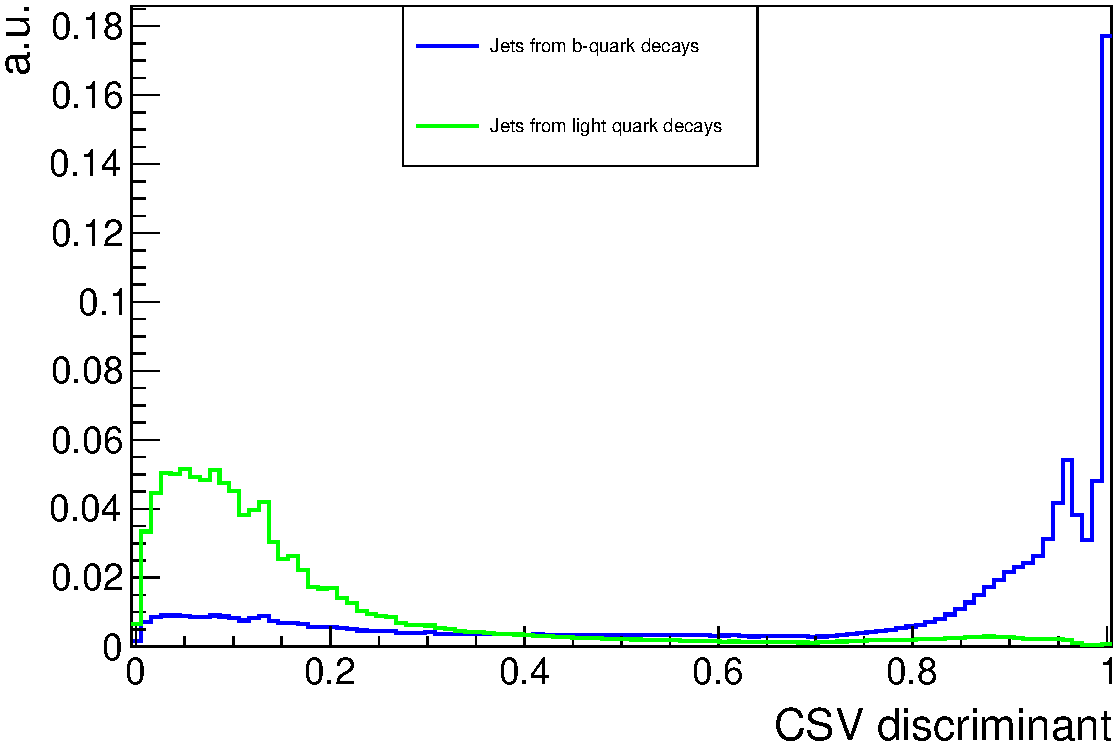
\includegraphics[width = 0.85 \textwidth]{Chapters/Chapter4_EvtSel/Figures/CSVDiscr_LightAndBJets.pdf}
 \caption{CSV discriminant} \label{fig::CSVDiscr}
\end{figure}

\begin{table}[h!t]
 \centering
 \caption{b-tag efficiency for the different working points of the CSV b-tagger.}
 \begin{tabular}{c|c|c|c|c}
  b-tag workin point 	& b-jet efficiency 	& udscg efficiency 	& c-jet efficiency 	& udsg efficiency 	\\
  \hline
  double Loose 		& 83.79 $\%$		& 18.91 $\%$		& 42.44 $\%$ 		& 13.4 $\%$		\\
  double Medium 	& 68.71 $\%$		& 4.57 $\%$		& 18.88 $\%$		& 1.21 $\%$		\\
  double Tight 		& 52.11 $\%$ 		& 1.22 $\%$ 		& 5.74 $\%$ 		& 0.16 $\%$ 		\\
 \end{tabular}
\end{table}


Since in this analysis emphasis lies on the correct reconstruction of the event topology, the choice of the b-tag working point has been based on the efficiency to precisely select the four jets present in the event. Hence, as was to be expected, the requirement of having at least two of these jets to be tagged using the most stringent working point results in the optimal reconstruction efficiency. As an additional bonus, this significantly reduces the event rates such that this additional event selection constraint also has a beneficial effect on the required processing time.
\\
With the b-tag working point fixed, the topology reconstruction proceeds by assigning the two most energetic jets surviving the b-tag requirement to the two jets originating from the b-quark decay. All other jets are then labelled as ``light jets'' and will need to be appointed \textbf{to the two} remaining jets in the event. 
In order to increase the efficiency of identifying the two correct light jets in the event the topology reconstruction has been adapted to consider the three most energetic light jets, if available, and assign the two most plausible ones to the jets produced during the hadronic decay of one of the W-bosons.
This choice again improves the topology reconstruction efficiency since for a significant number of events this third light jet is actually one of the correct jets.
\\
This light jet selection procedure is based on a $\chi^{2}$ method using both the mass of the lepton and the leptonic b and the mass of the hadronic b together with the two light quarks. Hence, this allows to, beside determining the two light jets, simultaneously distinguish the b-jet originating from the hadronic and the leptonic decaying top quark.
The expected values for both masses, denoted as $M_{lb}$ and $M_{qqb}$ respectively, have been determined using the semi-leptonically decaying top quarks with only the main event/the full event selection discussed up to now applied.\footnote{ (\textit{Why do you determine this before the b-tag? The b-tag will significantly influence the obtained mass values ... but will also reduce the available statistics ...} \textbf{Actually have also determined these values after the b-tags and the difference is almost negligible ...})}
The selection procedure then selects the event configuration for which these two mass values correspond the most with the expected values, taking into account their uncertainties.
\begin{equation}
 \chi^{2}_{M_{lb}, M_{qqb}} = \frac{(\hat{M_{lb}} - M_{lb})^{2}}{\sigma^{2}(\hat{M_{lb}})} + \frac{(\hat{M_{qqb}} - M_{qqb})^{2}}{\sigma^{2}(\hat{M_{qqb}})}
\end{equation}

An important motivation to use the $M_{lb}$ value in stead of the more obvious leptonic topquark mass is related to the difficult reconstruction of the neutrino.
Since only information on the $z$-component of this particle is available in particle detectors requires the determination of the $x$- and $y$-component the use of complex calculations based on the reconstructed masses. As a result it would not make much sense to reconstruct this particle, using the mass information, for then only using the leptonical top-quark mass. Especially since the $M_{lb}$ value can easily be reconstructed and fitted, although attention should be awarded to restrict the range where the fit is applied since this distribution is not expected to demonstrate the perfect Gaussian behaviour expected for the top quark mass.

\begin{table}[h!t]
 \centering
 \begin{tabular}{c|c|c|c}
		& $\hat{M_{lb}}$ ($\GeV$) 	& $\hat{M_{qqb}}$ ($\GeV$) 	& $\hat{M_{W}}$ ($\GeV$) 	\\
  \hline
  no b-tag 	& 106.9388 $\pm$ 32.0410 	& 174.5792 $\pm$ 17.5196 	& 83.7810 $\pm$ 10.2311 	\\
  b-tag 	& 107.7945 $\pm$ 32.4255 	& 175.0311 $\pm$ 17.0589 	& 83.6161 $\pm$ 10.2171 	
 \end{tabular}
 \caption{Obtained masses from Gaussian fit on distribution obtained before and after the application of the b-tagging requirement.}
\end{table}

Line
\\
\\
\textit{It is here that the choice of the two light jets takes place, in case of more than three light jets being present in the event!}\\
\textit{Will need to recalculate the numbers for the different b-tag options since the definition of light jets has changed ...} \\
\textit{And will also need to get these numbers for muon channel events alone ... Currently everything is done for muon and electron channel combined!}
\\
\\
\newpage
\paragraph{\underline{Comparing the 4 and 5 jet case for all the b-tags:}}
\subsubsection{4-jet case}
\begin{table}[!h] 
 \begin{tabular}{c|c|c|c|c|c} 
  \textbf{Option} & all 4 correct & $\geq$ 1 wrong       & correct ($\%$)       & $\frac{s}{b}$ & non-matched \\ \hline 
  2 L b-tags              & 426636 & 612386 & 41.0613 & 0.696678 & 1568843\\ 
  %2 L b-tags, light L-veto & 345646 & 487775 & 41.4732 & 0.708618 & 1268935\\ 
  2 M b-tags              & 325578 & 327020 & 49.8895 & 0.995591 & 826872\\ 
  %2 M b-tags, light M-veto & 310201 & 306237 & 50.3215 & 1.01294 & 783840\\ 
  %2 M b-tags, light L-veto & 237042 & 262674 & 47.4353 & 0.902419 & 625001\\ 
  2 T b-tags              & 198204 & 162941 & 54.8821 & 1.21642 & 422919\\ 
  %2 T b-tags, light T-veto & 195569 & 159603 & 55.0632 & 1.22535 & 415450\\ 
  %2 T b-tags, light M-veto & 181012 & 155451 & 53.7985 & 1.16443 & 394155\\ 
  %2 T b-tags, light L-veto & 138583 & 137450 & 50.2052 & 1.00824 & 317064\\ 
 \end{tabular} 
 \caption{Overview of correct and wrong reconstructed events for the different b-tags (no $\chi^{2}$ $m_{lb}$ - $m_{qqb}$ applied)}
\end{table} 
 
\begin{table}[!h] 
 \begin{tabular}{c|c|c|c|c|c} 
  \textbf{Option} & 2 b's correct & $\geq$ 1 b wrong     & b's correct ($\%$)   & $\frac{s}{b}$ & non-matched \\ \hline 
  2 L b-tags              & 589953 & 449069 & 56.7796 & 1.31372 & 1568843\\ 
  %2 L b-tags, light L-veto & 500672 & 332749 & 60.0743 & 1.50465 & 1268935\\ 
  2 M b-tags              & 460691 & 191907 & 70.5934 & 2.4006 & 826872\\ 
  %2 M b-tags, light M-veto & 445064 & 171374 & 72.1993 & 2.59703 & 783840\\ 
  %2 M b-tags, light L-veto & 360899 & 138817 & 72.2208 & 2.59982 & 625001\\ 
  2 T b-tags              & 280306 & 80839 & 77.6159 & 3.46746 & 422919\\ 
  %2 T b-tags, light T-veto & 277571 & 77601 & 78.1511 & 3.5769 & 415450\\ 
  %2 T b-tags, light M-veto & 263210 & 73253 & 78.2285 & 3.59316 & 394155\\ 
  %2 T b-tags, light L-veto & 213584 & 62449 & 77.3763 & 3.42013 & 317064\\ 
 \end{tabular} 
 \caption{Overview of correct and wrong reconstructed b-jets for the different b-tags (no $\chi^{2}$ $m_{lb}$ - $m_{qqb}$ applied)}
\end{table} 
 
\begin{table}[!h] 
 \begin{tabular}{c|c|c|c|c|c} 
  \textbf{Option} & 2 light good  & $\geq$ 1 light wrong & light correct ($\%$) & $\frac{s}{b}$ & non-matched \\ \hline 
  2 L b-tags              & 504181 & 534841 & 48.5246 & 0.942675 & 1568843\\ 
  %2 L b-tags, light L-veto & 415812 & 417609 & 49.8922 & 0.995697 & 1268935\\ 
  2 M b-tags              & 374193 & 278405 & 57.339 & 1.34406 & 826872\\ 
  %2 M b-tags, light M-veto & 358096 & 258342 & 58.0912 & 1.38613 & 783840\\ 
  %2 M b-tags, light L-veto & 274331 & 225385 & 54.8974 & 1.21717 & 625001\\ 
  2 T b-tags              & 227716 & 133429 & 63.0539 & 1.70665 & 422919\\ 
  %2 T b-tags, light T-veto & 225072 & 130100 & 63.3699 & 1.72999 & 415450\\ 
  %2 T b-tags, light M-veto & 209171 & 127292 & 62.1676 & 1.64324 & 394155\\ 
  %2 T b-tags, light L-veto & 160090 & 115943 & 57.9967 & 1.38076 & 317064\\ 
 \end{tabular} 
 \caption{Overview of correct and wrong reconstructed light jets for the different b-tags (no $\chi^{2}$ $m_{lb}$ - $m_{qqb}$ applied)}
\end{table} 

\newpage
\subsubsection{5-jet case}
\begin{table}[!h] 
 \begin{tabular}{c|c|c|c|c|c} 
  \textbf{Option} & all 4 correct & $\geq$ 1 wrong       & correct ($\%$)       & $\frac{s}{b}$ & non-matched \\ \hline 
  2 L b-tags              & 512367 & 526655 & 49.3124 & 0.97287 & 1568843\\ 
  %2 L b-tags, light L-veto & 410486 & 422935 & 49.2531 & 0.970565 & 1268935\\ 
  2 M b-tags              & 396904 & 255694 & 60.8191 & 1.55226 & 826872\\ 
  %2 M b-tags, light M-veto & 377217 & 239221 & 61.193 & 1.57686 & 783840\\ 
  %2 M b-tags, light L-veto & 282672 & 217044 & 56.5665 & 1.30237 & 625001\\ 
  2 T b-tags              & 241394 & 119751 & 66.8413 & 2.0158 & 422919\\ 
  %2 T b-tags, light T-veto & 238024 & 117148 & 67.0165 & 2.03182 & 415450\\ 
  %2 T b-tags, light M-veto & 219617 & 116846 & 65.2723 & 1.87954 & 394155\\ 
  %2 T b-tags, light L-veto & 164817 & 111216 & 59.7092 & 1.48195 & 317064\\ 
 \end{tabular} 
 \caption{Overview of correct and wrong reconstructed events for the different b-tags (no $\chi^{2}$ $m_{lb}$ - $m_{qqb}$ applied, 5 jets considered)}
\end{table} 
 
\begin{table}[!h] 
 \begin{tabular}{c|c|c|c|c|c} 
  \textbf{Option} & 2 b's correct & $\geq$ 1 b wrong     & b's correct ($\%$)   & $\frac{s}{b}$ & non-matched \\ \hline 
  2 L b-tags              & 589953 & 449069 & 56.7796 & 1.31372 & 1568843\\ 
  %2 L b-tags, light L-veto & 500672 & 332749 & 60.0743 & 1.50465 & 1268935\\ 
  2 M b-tags              & 460691 & 191907 & 70.5934 & 2.4006 & 826872\\ 
  %2 M b-tags, light M-veto & 445064 & 171374 & 72.1993 & 2.59703 & 783840\\ 
  %2 M b-tags, light L-veto & 360899 & 138817 & 72.2208 & 2.59982 & 625001\\ 
  2 T b-tags              & 280306 & 80839 & 77.6159 & 3.46746 & 422919\\ 
  %2 T b-tags, light T-veto & 277571 & 77601 & 78.1511 & 3.5769 & 415450\\ 
  %2 T b-tags, light M-veto & 263210 & 73253 & 78.2285 & 3.59316 & 394155\\ 
  %2 T b-tags, light L-veto & 213584 & 62449 & 77.3763 & 3.42013 & 317064\\ 
 \end{tabular} 
 \caption{Overview of correct and wrong reconstructed b-jets for the different b-tags (no $\chi^{2}$ $m_{lb}$ - $m_{qqb}$ applied, 5 jets considered)}
\end{table} 
 
\begin{table}[!h] 
 \begin{tabular}{c|c|c|c|c|c} 
  \textbf{Option} & 2 light good  & $\geq$ 1 light wrong & light correct ($\%$) & $\frac{s}{b}$ & non-matched \\ \hline 
  2 L b-tags              & 603601 & 435421 & 58.0932 & 1.38625 & 1568843\\ 
  %2 L b-tags, light L-veto & 493376 & 340045 & 59.1989 & 1.45091 & 1268935\\ 
  2 M b-tags              & 452953 & 199645 & 69.4077 & 2.26879 & 826872\\ 
  %2 M b-tags, light M-veto & 432443 & 183995 & 70.1519 & 2.3503 & 783840\\ 
  %2 M b-tags, light L-veto & 324766 & 174950 & 64.9901 & 1.85634 & 625001\\ 
  2 T b-tags              & 275125 & 86020 & 76.1813 & 3.19838 & 422919\\ 
  %2 T b-tags, light T-veto & 271763 & 83409 & 76.5159 & 3.2582 & 415450\\ 
  %2 T b-tags, light M-veto & 251381 & 85082 & 74.7128 & 2.95457 & 394155\\ 
  %2 T b-tags, light L-veto & 188773 & 87260 & 68.3878 & 2.16334 & 317064\\ 
 \end{tabular} 
 \caption{Overview of correct and wrong reconstructed light jets for the different b-tags (no $\chi^{2}$ $m_{lb}$ - $m_{qqb}$ applied, 5 jets considered)}
\end{table} 
 

\newpage
\subsection{Number of light jets}

\subsection{Signal optimisation}\label{subsec::MassCuts}

\subsection{Data-MC agreement}\label{subsec::DataMC}
%\chapter{The Matrix Element method} \label{ch::MW}

The measurement of the right-handed tensor coupling of the Wtb interaction discussed in this thesis is performed using the Matrix Element method.
This is an advanced analysis technique which allows to extract theoretical information from experimental events without requiring prior knowledge of the possible new-physics scenarios.
%The method finds its name in the fact that 
%\textit{The Matrix Element method has been developed several years ago and has been used extensively at the Tevatron, especially in the top-quark physics sector.}
%\\
\\
The Matrix Element method assigns a probability to each theoretical hypothesis on an event-by-event basis, by calculating the matrix element of the considered process.
The obtained event probabilities are then combined into a likelihood and the most probable hypothesis is determined using a likelihood-maximisation method.
\\
\\
A detailed overview of the technicalities and applicability of the Matrix Element method can be found in this Chapter.
At first, the theoretical framework used to calculate these event probabilities will be discussed in Section~\ref{sec::MWTheory}.
In order to demonstrate the use of the Matrix Element method, the measurement of the top-quark mass will be presented as an example/feasibility study in Section~\ref{sec::MEMExample}.

\section{Theoretical framework (IMPROVE)} \label{sec::MWTheory}

The Matrix Element method has been developed several years ago in order to make maximal use of the kinematic information available.
Since this method capable of analysing processes with a complex final state, typically containing several jets and missing energy, it has been used extensively in the top-quark physics sector at the Tevatron~\cite{MEMTevatron}.
Given the challenging conditions the LHC is faced with, the use of the Matrix Element method has been revived recently and it has found applications in different physics areas; including the discovery of the Brout-Englert-Higgs boson~\cite{HiggsMEM}.
\\
\\
The fact that the Matrix Element is capable of dealing in an efficient manner with event signatures involving missing energy together with the option it provides to determine the most optimal theoretical parameter of any imposed theoretical model\footnote{The Matrix Element method also has a second widely used application, where it analyses two competing hypotheses and determines which one corresponds the most with the available experimental information.}, has made it the appropriate analysis technique to use for the measurement of the $\gR$ coefficient.
\\

Section~\ref{subsec::MWLik} will focus on the determination of the Matrix Element method and the procedure followed to calculate the matrix-elements of each event. Section~\ref{subsec::FRModel} will discuss the details of the imposed theoretical model specifically developed for the study of the anomalous couplings in the Wtb interaction vertex.

\subsection{Likelihood definition and evaluation} \label{subsec::MWLik}

The probability for each experimental event to agree with the considered theoretical model, for which the information is provided by the squared matrix-element, 
is defined as:
\begin{equation} \label{eq::MWEvtProb}
 P(x \vert \alpha) = \frac{1}{\sigma_{\alpha}} \int d\Phi(y) \, dq_{1} \, dq_{2} ~ f_{1}(q_{1}) \, f_{2}(q_{2}) \, \vert M_{\alpha}(y) \vert^{2} \, W(x,y)
\end{equation}
with $x$ the reconstructed event, $y$ the parton-level configuration, $\alpha$ the set of parameters, $\vert M_{\alpha}(y) \vert^{2}$ the squared matrix-element, d$\Phi$ the phase-space measure, $f_{i}(q_{i})$ the parton distribution functions and $W(x,y)$ the resolution or transfer function.
\\
This resolution function, which will be discussed in detail in Section~\ref{sec::TF}, ensures the detector effects influencing the reconstructed events are transfered to the parton-level configuration.
Normalising the obtained event weight with the total cross-section $\sigma_{\alpha}$ is necessary in order to obtain a probability density. Hence this should incorporate both the different cross-section values of the process and the different selection efficiency when varying the theoretical parameter $\alpha$ in the considered model. 
More detail on this normalisation procedure will be given in Section~\ref{sec::Norm}.
\\

The overall likelihood $\mathcal{L}_{MEM}$ from which the Matrix Element method will extract the most optimal value of the theoretical parameter $\alpha$, is obtained by multiplying all these individual event probabilities. The actual extraction is done by minimising these likelihood values.
\begin{equation}
 \mathcal{L}_{MEM}(x \vert \alpha) = \prod_{i=1}^{n} P(x \vert \alpha)
\end{equation}
In practice it is more convenient to convert the likelihood values using $\chi^{2}$ = $-2 \ln \mathcal{L}$ such that the log-likelihood curves of the event can be summed and that the overall $\DeltaChi$ = $\chi^{2}_{MEM} - \chi^{2}_{MEM,min}$ can be minimised. \textbf{Mention this MEM estimator stuff ...}
\begin{equation}
 \chi^{2}(x \vert \alpha) = -2 \ln \mathcal{L}_{MEM}(x \vert \alpha) = -2 \sum_{i=1}^{n} \ln P(x \vert \alpha)
\end{equation}

The Matrix Element method is supposed to provide the most powerful tool to extract theoretical information from a sample of experimental events.
However, the applicability of the method is seriously limited by the challenging computation procedure of the individual event probabilities.
The evaluation of each individual event requires a non-trivial multi-dimensional integration over the combined theoretical the hard-scattering process, and the experimental information, the transfer functions.
Hence even to analyse a limited data sample, a significant processing time has to be foreseen.
\\
\\
Due to the increasing number of possible applications of the Matrix Element method at the LHC and in phenomenological studies, a dedicated algorithm aimed at evaluating these event weights using a fully automated approach has been developed. This highly flexible phase-space generator (\textbf{not integrator?}), which uses the adaptive Monte Carlo integrator VEGAS~\cite{VEGAS}, has been denoted as MadWeight~\cite{MadWeightPaper}.
%\\
Before this tool was available, a separate integration procedure had to be developed for each considered process and detailed knowledge on the technical details of both matrix-element generation and phase-space integration was required to apply the Matrix Element method.
%\textit{This is no longer the case since the MadWeight integrator optimises the phase-space mapping.}
%***********************
% The notation of calling MadWeight a phase-space generator can be found on their twiki!!
% https://cp3.irmp.ucl.ac.be/projects/madgraph/wiki/MadWeight
%***********************
\\

%Now mention the fact that it is still slow and thus a stringent event selection has been asked for + limited the permutations of the b-jets!
Even with the implementation of the MadWeight integrator, the Matrix Element method remains a very time-consuming analysis technique.
Therefore it should be avoided to calculate the probabilities of events for which the expected final state particles are not, or incompletely, recovered; hence the stringent event-selection criteria imposed in Chapter~\ref{ch::EvtSel}.
Also the choice to distinguish the two b-quark jets originating from the W-boson decay in top-quark pair events has been applied for the purpose of reducing the necessary computing time, since this reduces the number of permutations to be considered with a factor of $2$.
Hence for this analysis, where the semi-muonic decay of the $\ttbar$ events is studied, this implies that only the permutations between the two light jets have to be performed during the integration procedure. 


\subsection{Implementation of the anomalous Wtb Lagrangian} \label{subsec::FRModel}

Since it has been opted for to implement the MadWeight integration procedure in the MadGraph framework, the option to analyse personally created theoretical models describing new-physics phenomena has been significantly facilitated.
%\textit{This approach allows to go from theory to simulation to comparison with experiment in a quick, efficient and accurate manner (Not completely own words!)}
%\\
Hence, any model can be created with FeynRules~\cite{FeynRules}, which is a Mathematica-based package to calculate Feynman rules, and be translated to MadGraph using the dedicated interface.
The developed model should only contain some basic information, such as the particle content, the parameters and the lagrangian, which allows the FeynRules package to derive the Feynman rules.
\\

In this analysis a new model has been created using this FeynRules package since no anomalous couplings for the top-quark pair decay vertex are expected in the Standard Model Lagrangian.
This so-called Wtb-model is constructed as an addition of the Standard Model, hence the entire particle content and parameters of this model has been kept.
The description of the anomalous couplings is then included by introducing four new complex parameters, the four coupling coefficients, and the full lagrangian described in Equation (\ref{eq::FullWtbLagr}).
Since the parameter of interest for this analysis, the $\gR$ coefficient of this Wtb interaction vertex, is associated with the decay of the top-quark and is thus not foreseen to change the final state particles, the particle content has not been altered.
\\
Within the model some simplifications have been added since the complexity of the developed model is directly related to the processing time needed for the MadWeight integration procedure to evaluate an event. %described by the introduced theoretical model.
Hence, the light-flavoured quarks (u-, d-, c- and s-quark) are assumed to be massless and, just as is the case for the Standard Model decays, the CKM-suppressed W-boson decays have been suppressed.
\\

Besides calculating the Feynman rules for the developed theoretical model, the FeynRules package also ensures the introduced lagrangian fulfills the basic set of requirements, such as hermicity, gauge invariance, $etc. $.
Nevertheless, the downside of developing such a brand new model is that there is no straightforward way to determine whether the obtained output for the various unknown parameters \textit{corresponds to the expectations/is well described}.
For the top-quark decay interaction vertex some influences of the coupling coefficients can be visualised by looking at the distortions of the angular distribution of the \textbf{top-quark decay products}, as has been mentioned in Section~\ref{sec::SubWtb}. 
Hence, a thorough comparison has been performed with the distributions obtained when simulating events with different values for the coupling coefficients using the developed Wtb-model, resulting in an excellent agreement as can be seen in Figure~\ref{fig::ModelTest}.
In addition, the model has also been used to calculate the most optimal value of some of the well-known parameters of the Standard Model, for which no unexpected deviations have been observed. 

\begin{figure}[h!t]
 \centering
 
\includegraphics[width = 0.3 \textwidth]{image.png}
 \caption{\textbf{Comparison between theory and MadGraph model output.}} \label{fig::ModelTest}
\end{figure}


\section{Resolution functions} \label{sec::TF}

As mentioned in the previous section, the Matrix Element method uses the parton-level information extracted from the actual matrix element of the considered theoretical model to calculate the event probability.
Hence, in order to \textit{match/link} the three momenta of these final-state \textit{particles/partons} with the corresponding momenta of the reconstructed physics objects, carefully calculated resolution functions are \textit{required/needed/necessary}. 
\\
\textbf{Combined effect of parton showering, hadronisation and detector response.}
\\
\\
Nevertheless (its importance), this aspect of the Matrix Element method has some strong simplifications imposed.
Since such a resolution function should be determined for each particle type, describing both its direction ($\phi$ and $\theta$) and energy, it is assumed that these functions are uncorrelated.
This allows to reformulate the resolution function $W(x,y)$ in Equation (\ref{eq::MWEvtProb}) using a factorised approach:
\begin{equation}
 W(x,y) = \prod_{i}^{N} W(x_i, y_i) = \prod_{i}^{N} W_{i}^{E}(x^{i},y^i) \, W_{i}^{\eta}(x^i, y^i) \, W_{i}^{\phi}(x^i,y^i)
\end{equation}
where the index $i$ runs over the different types of physics objects in the considered event topology.
\\
\\
This \textit{factorised} description can be simplified even further since (\textit{the transfer functions of}) both object directions can be respresented with a Dirac-$\delta$ function.
This because both angles are determined very precisely (\textit{in the CMS detector/hadron detectors}) and therefore correspond very well with the measured objects, as can be seen from Figure~\ref{fig::TFAngles}. The differences shown in these distributions are determined using the parton-level and reconstructed physics object to have an angular distance $\Delta R$ smaller than 0.3, a similar condition as what is applied in Chapter~\ref{ch::EvtSel}.
As a result, the only remaining phase-space variable for which a transfer function should be determined is the energy, for which the introduced assumption is not correct due to the finite resolution on its measurement. The transfer function of the energy variable will therefore be represented with a Gaussian-like function.
\\
\begin{figure}[h!tp]
 \centering
 
\includegraphics[width = 0.31 \textwidth]{image.png} \hspace{0.1cm} 
 
\includegraphics[width = 0.31 \textwidth]{image.png} \hspace{0.1cm}
 
\includegraphics[width = 0.31 \textwidth]{image.png}
 \caption{Draw the $\Delta \phi$ and $\Delta \theta$ to show this is very narrow! + Show difference with $\Delta E$. (Kinematic variables are the ones with all corrections as discussed in Chapter~\ref{ch::EvtSel})} \label{fig::TFAngles}
\end{figure}

In this analysis, which focusses on the semi-muonic decay of top-quark pairs, a dedicated transfer function should be developed for the jets and the muon in the event.
However, due to the possible different behaviour of the light- and heavy-flavoured jets, it has been opted for to determine two separate transfer functions for the jets.
Hence, the two jets identified as originating from the decay of the W-boson and the two jets assigned to the b-quark decay will be treated independently. 
The transfer function for the muons on the other hand will also be represented with a Dirac-$\delta$ function since its energy is determined very precisely. The different behaviour for the muon and the jets, the light-flavoured ones in this case, can be seen in Figure~\ref{fig::TFJetEDistr}.
%\textit{Looking at the energy difference for the muons also indicated that this is actually determined very precisely and can therefore also be respresented with a Dirac-$\delta$ function.}
\\
Besides simplifying the transfer-function calculation, this approach of using Dirac-$\delta$ functions for various phase-space variables and particles also significantly speeds up the Matrix Element method.
Fixing the properties of the reconstructed objects to those of the parton-level ones implies that the method does not have to integrate over the corresponding phase-space variables.
%*****************************************
% This non-integration is mentioned on page 3 of main MadWeight paper (discusses there the ideal case of no TF)
%*****************************************
\\
\begin{figure}[h!tp]
 \centering
 
\includegraphics[width = 0.3 \textwidth]{image.png} \hspace{0.2cm}
 
\includegraphics[width = 0.3 \textwidth]{image.png} \\ \vspace{0.2cm}
 
\includegraphics[width = 0.3 \textwidth]{image.png} \hspace{0.2cm}
 
\includegraphics[width = 0.3 \textwidth]{image.png}
 \caption{$Delta E$ distributions for different parton energies.} \label{fig::TFJetEDistr}
\end{figure}

The transfer function of the both the light- and heavy-flavoured jets will be described using a double-Gaussian distribution, for which the formula is given in Equation (\ref{eq::DblGausTF}).
%The factor $(a_2 + a_3 a_5)$ ensures the obtained transfer function is normalised such that the event-probability remains a probability density.
This double-Gaussian representation is the optimal choice to describe the energy difference ($\Delta E$ = $E_{parton}$ - $E_{jet}$) of jets, which is characterised by a sharp peak combined with an asymmetric tail. 
From Figure~\ref{fig::TFJetEDistr} can furthermore be concluded that the width of the overall $\Delta E$ distribution increases for higher energies of the matched parton. Hence an accurate description of both the peak and the tail is necessary in order to ensure the transfer function remains valid for a wide energy regime.
\begin{equation} \label{eq::DblGausTF}
 W^{E}(parton, jet) = \frac{1}{\sqrt{2\pi}} \frac{1}{a_2 + a_3 a_5} \left( \exp \frac{-(\Delta E - a_1)^2}{2 a_2 \,^{2}} + a_3 \exp \frac{-(\Delta E - a_4)^2}{2 a_5 \,^{2}} \right) 
\end{equation}
where the parameters $a_1$ and $a_4$ represent the mean of the first and second Gaussian, respectively, while the parameters $a_2$ and $a_5$ give the width of those respective Gaussian distributions.
The remaining parameter $a_3$ takes into account the relative contribution of both distributions.
\\

The actual determination of the two remaining transfer functions will be performed by applying a double-Gaussian fit on the obtained $\Delta E$ distribution for various $E_{parton}$ values.
For the light jets 16 bins are considered between $25 \GeV$ and $160 \GeV$, while for the b-quark jets 18 bins are used between $30 \GeV$ and $230 \GeV$.
In order to ensure sufficient statistics is available throughout the entire energy-range, only the basic event-selection requirements have been applied. So the fine-tuning criteria discussed in Section~\ref{sec::SpecificSelec} are not taken into account when determining the transfer functions.
\\
Hence for each of the considered $E_{parton}$-bins a measurement of the five $E$-dependent parameters representing the double-Gaussian transfer function is obtained.
The $E$-dependency of these transfer-function parameters is based on the parametrisation of the calorimeter energy resolution, which corresponds to $y$ = $a + b \sqrt{E} + c E$.
However, in order to ensure the parameters are well described by this parameterisation, a quadratic term, or for some parameters even a cubic term, has been added. An overview of the imposed $E$-dependency for the different $a_i$ parameters can be found in Table~\ref{table::EDependency}.
\\
\begin{table}[h!tp]
 \centering
 \caption{Imposed $E$-dependency of the different transfer-function parameters. Only in three cases the additional cubic function was necessary to obain a good description of the corresponding parameter.} \label{table::EDependency}
 \renewcommand{\arraystretch}{1.2}
 \begin{tabular}{|c|c|}
  \hline
  Light-jet parameters 								& b-quark jet parameters 							\\
  \hline
  $a_{1,0} + a_{1,1}\sqrt{E} + a_{1,2} E + a_{1,3} E^{2} + a_{1,4} E^{3}$ 	& $a_{1,0} + a_{1,1}\sqrt{E} + a_{1,2} E + a_{1,3} E^{2} + a_{1,4} E^{3}$ 	\\
  $a_{2,0} + a_{2,1}\sqrt{E} + a_{2,2} E + a_{2,3} E^{2}$ 			& $a_{2,0} + a_{2,1}\sqrt{E} + a_{2,2} E + a_{2,3} E^{2}$		 	\\
  $a_{3,0} + a_{3,1}\sqrt{E} + a_{3,2} E + a_{3,3} E^{2}$		 	& $a_{3,0} + a_{3,1}\sqrt{E} + a_{3,2} E + a_{3,3} E^{2} + a_{3,4} E^{3}$ 	\\
  $a_{4,0} + a_{4,1}\sqrt{E} + a_{4,2} E + a_{4,3} E^{2}$		 	& $a_{4,0} + a_{4,1}\sqrt{E} + a_{4,2} E + a_{4,3} E^{2}$		 	\\
  $a_{5,0} + a_{5,1}\sqrt{E} + a_{5,2} E + a_{5,3} E^{2}$		 	& $a_{5,0} + a_{5,1}\sqrt{E} + a_{5,2} E + a_{5,3} E^{2}$ 			\\
  \hline
 \end{tabular}
\end{table}

The two-dimensional histogram showing the $E_{parton}$ distribution with respect to the $\Delta E$ distribution for both the light- and heavy-flavoured jets can be found in Figure~\ref{fig::TF2DPlot}, respectively the left and right plot.
Comparing the two distributions allows to conclude that it is indeed beneficial to treat both types of jets independently since a wider $\Delta E$ distribution is clearly visible for the b-quark jets.
\\
Figure~\ref{fig::TFSlices} contains some examples of the $\Delta E$ distribution obtained for some specific parton-level energy bins. The two upper plots correspond to the light-flavoured jets while the two lower ones depict the situation for the heavy-flavoured ones.
In order to visualise the importance of using a double-Gaussian description for the transfer functions of the jet energies, the left distribution gives the distribution for the relatively low parton energies while the right corresponds to one of the more outer bins of the considered energy range.
As can be seen, the range where the double-Gaussian fit is applied has been optimised for each of the considered bins of $E_{parton}$.

\begin{figure}[h!tp]
 \centering
 \includegraphics[width = 0.45 \textwidth]{Chapters/Chapter5_MadWeight/Figures/Light_DiffEVsGenE.pdf} \hspace{0.2cm}
 \includegraphics[width = 0.45 \textwidth]{Chapters/Chapter5_MadWeight/Figures/BJet_DiffEVsGenE.pdf} 
 \caption{Two-dimensional histogram showing the parton energy $E_{parton}$ with respect to the difference in energy with the matched jet, $\Delta E$ for the light jets (left) and the b-quark jets (right). The transfer-function is determined from these histograms by fitting the $y$-axis projection of each considered $x$-axis bin with a double-Gaussian.} \label{fig::TF2DPlot}
\end{figure}

\begin{figure}[h!tp]
 \centering
 \includegraphics[width = 0.45 \textwidth]{Chapters/Chapter5_MadWeight/Figures/sliceYbin2And3_Light_DiffEVsGenE.pdf} \hspace{0.2cm}
 \includegraphics[width = 0.45 \textwidth]{Chapters/Chapter5_MadWeight/Figures/sliceYbin12And13_Light_DiffEVsGenE.pdf} \vspace{0.1cm} \\
 \includegraphics[width = 0.45 \textwidth]{Chapters/Chapter5_MadWeight/Figures/sliceYbin3_BJet_DiffEVsGenE.pdf} \hspace{0.2cm}
 \includegraphics[width = 0.45 \textwidth]{Chapters/Chapter5_MadWeight/Figures/sliceYbin12And14_BJet_DiffEVsGenE.pdf}
 \caption{Distribution of the difference in energy between the parton-level and reconstructed object for both the light jets (upper two) and the b-quark jets (lower two) fitted with a double-Gaussian function. The different shape for lower (left) and higher (right) energy values is clearly visible.} 
\end{figure}

Finally, the obtained $E$-dependent shape of the five parameters describing the double-Gaussian transfer function is given in Figure~\ref{fig::TFLight} and \ref{fig::TFBJet} for the light and b-quark jets, respectively. In case some of the considered $\Delta E$ distributions was low on statistics, it has been combined with one of the surrounding bins in order to ensure sufficient information was available for the double-Gaussian fit.
This effect is clearly visible in the depicted measurement points, especially at the edges of the considered energy range where the number of events started to decrease.

\begin{figure}[h!tp]
 \centering
 \includegraphics[width = 0.46 \textwidth]{Chapters/Chapter5_MadWeight/Figures/Light_DiffEVsGenE_a1_Fit.pdf} \hspace{0.2cm}
 \includegraphics[width = 0.46 \textwidth]{Chapters/Chapter5_MadWeight/Figures/Light_DiffEVsGenE_a2_Fit.pdf} \vspace{0.3cm} \\
 \includegraphics[width = 0.46 \textwidth]{Chapters/Chapter5_MadWeight/Figures/Light_DiffEVsGenE_a3_Fit.pdf} \hspace{0.2cm}
 \includegraphics[width = 0.46 \textwidth]{Chapters/Chapter5_MadWeight/Figures/Light_DiffEVsGenE_a4_Fit.pdf} \vspace{0.3cm} \\
 \includegraphics[width = 0.46 \textwidth]{Chapters/Chapter5_MadWeight/Figures/Light_DiffEVsGenE_a5_Fit.pdf}
 \caption{Obtained shape for the five $E$-dependent parameters describing the double-Gaussian transfer function for the light-flavoured jets. This has been fitted with the corresponding parametrisation given in Table~\ref{table::EDependency}.} \label{fig::TFLight}
\end{figure}

\begin{figure}[h!tp]
 \centering
 \includegraphics[width = 0.46 \textwidth]{Chapters/Chapter5_MadWeight/Figures/BJet_DiffEVsGenE_a1_Fit.pdf} \hspace{0.2cm}
 \includegraphics[width = 0.46 \textwidth]{Chapters/Chapter5_MadWeight/Figures/BJet_DiffEVsGenE_a2_Fit.pdf} \vspace{0.2cm} \\
 \includegraphics[width = 0.46 \textwidth]{Chapters/Chapter5_MadWeight/Figures/BJet_DiffEVsGenE_a3_Fit.pdf} \hspace{0.2cm}
 \includegraphics[width = 0.46 \textwidth]{Chapters/Chapter5_MadWeight/Figures/BJet_DiffEVsGenE_a4_Fit.pdf} \vspace{0.2cm} \\
 \includegraphics[width = 0.46 \textwidth]{Chapters/Chapter5_MadWeight/Figures/BJet_DiffEVsGenE_a5_Fit.pdf}
 \caption{Obtained shape for the five $E$-dependent parameters describing the double-Gaussian jet transfer function for the b-flavoured jets. This has been fitted with the corresponding parametrisation given in Table~\ref{table::EDependency}.} \label{fig::TFBJet}
\end{figure}

~~~

%Due to the introduced assumptions, the applicability of the Matrix Element method will need to be tested in detail in order to ensure it is not affected by a bias, as will be discussed in Section~\ref{sec::EstimatorProp}.
%\\
%\textit{But in my case linearity test is not performed using the Transfer Functions discussed here!!}

\section{Cross-section  normalisation} \label{sec::Norm}
\textit{Since it is here a rather general case, first the method for generator-level events can be mentioned and then the difference with reconstructed collision events can be made perfectly clear.}

An important aspect of the Matrix Element method is the normalisation of the event probability using the cross-section and acceptance, which might vary significantly for the considered configurations. For the top-quark mass example given in Section~\ref{sec::TopMass}, the effect of this normalisation was negligible but for the measurement of the anomalous coupling coefficient this factor has proven to be rather important. The method opted for in this analysis to determine these cross-section values will be explained in Section~\ref{subsec::XSReco}.

For the measurement of the right-handed tensor coupling the cross-section normalisation is a vital component.
Independent whether generator-level or reconstructed events are considered, without this normalisation applied the Matrix Element method does not result in the correct outcome.
The substantial influence of this normalisation component has been summarised in Figure~\ref{fig::XSInflGen}, which shows the overall $\chiSqMEM$ distribution prior to and after the cross-section normalisation has been taken into account. The considered sample has been created using the Standard Model configuration such that the minimum of the distribution should correspond to $0$.
%This because the observed variations of the overall event probability for the coupling coefficient are much smaller than was the case for the top-quark mass measurement such that the cross-section normalisation actually has a significant influence on the obtained outcome.
%***********************************
% --> Certain this is the reason?
% ==> Maybe good to think of an explanation why this cross-section normalisation is so much more important
%***********************************
\begin{figure}[h!t]
 \centering
 % Add here the gR gen-level result of FitDistributions_CalibCurve_SemiMu_RgR_AllDeltaTF_MGSampleSM_20000Evts_NoCuts_OuterBinsExclForFit_20000Evts.root with and without XS normalisation
 % Important: Cannot yet use the sample after the event-selection is applied because this still has to be explained!!
 % --> Do this without the fit maybe .. ?
 
\includegraphics[width = 0.3 \textwidth]{image.png} \hspace{0.5cm}
 
\includegraphics[width = 0.3 \textwidth]{image.png}
 \caption{Distribution of the overall $\chiSqMEM$-value obtained by analysing the right-handed tensor coupling using 20 000 generator-level events. The distribution on the left is without any normalisation applied while the right one corresponds to the normalised result.} \label{fig::XSInflGen}
\end{figure}

The significant impact of the cross-section normalisation on the outcome of the measurement implies that the cross-section values for the reconstructed-level analysis should be determined with great care.
However, in contrast to the easy access to generator-level samples with alternative coupling coefficients, generating similar samples containing reconstructed events is a rather challenging and time-consuming process.
As a result, it has been opted for in this thesis to derive the cross-section values for the reconstructed events from the generator-level ones.
This approach significantly facilitates the cross-section determination since any generated process by MadGraph automatically calculates the cross-section of the considered process.
%**********************
% Any other motivation why FastSim has not been considered?
% --> Certain that it would perfectly describe the SM samples??
%**********************
\\
\\
In order to ensure that the obtained generator-level cross-sections can easily be related to the reconstructed ones, the conditions present for the reconstructed collision events will be mimicked as closely as possible during the generation process. Hence the generator events have to fullfill the basic event selection requirements\footnote{Important to note here is that once these selection criteria are applied to the generated events, the obtained cross-section will actually be a combination of the cross-section of the underlying physics process and the acceptance of the considered event selection. Hence the term ``cross-section normalisation'' will \textbf{implicitely} imply the combined normalisation $\sigma \times A$ mentioned in Equation~\ref{eq::MWEvtProb}.} listed in Table~\ref{table::GenCuts}.
By applying a significant fraction of the full event selection chain onto the generated events, the expected relative difference in behaviour of each $\gR$ value on the considered kinematic constraints will be incorporated. As previously mentioned in Section~\ref{sec::CalibCurve}, the remaining event-selection criteria are supposed to be less sensitive to the value of the coupling coefficient.
%The remaining event selection criteria are believed to be less sensitive to the value of the coupling coefficient, thus their relative dependence will not be taken into account.
\\
\\
In addition, the generated processes are also selected in order to remain with a similar event signature as is the case in data. Hence the cross-section values have been determined using a combination of top-quark pair decay processes surrounded with additional jets. The actual number of considered processes has been limited to the $\ttbar$ decay with none, one and two additional jets since the contribution of the following decays quickly becomes negligible.
%********************************************
% --> Does this correspond to LO, NLO and NNLO or is this still something different??
% Question: Interesting to give some of the Feynman diagrams belonging to the different processes?
%********************************************
\begin{figure}[h!t]
 \centering
 
\includegraphics[width = 0.15 \textwidth]{image.png} \hspace{0.2cm}
 
\includegraphics[width = 0.15 \textwidth]{image.png} \hspace{0.2cm}
 
\includegraphics[width = 0.15 \textwidth]{image.png}
 \caption{Feynman diagrams for the different generator-level processes considered for the calculation of the cross-sections. \textbf{Relevant?}}
\end{figure}

Even with these two optimisations applied, this approach will not result in a perfect agreement with the selected events. For instance, it is simply not possible to include every aspect of the full event-selection chain in exactly the same way when generating the different processes.
Hence, the obtained cross-section values will be scaled in order to take into account the influence of these non-included event selection criteria.
For this an identical behaviour throughout the entire $\gR$ range is assumed such that each cross-section value will be multiplied with the factor $\sigma_{SM}^{reco}$/$\sigma_{SM}^{gen}$. 
%********************************************
% --> Think of any other non-included effects!!
%********************************************
\\
In this factor the term $\sigma_{SM}^{reco}$ represents the measured cross-section of the selected events while the cross-section obtained for the combined generator-level sample created using the Standard Model configuration is denoted by $\sigma_{SM}^{gen}$.
The cross-section of the selected events is determined by dividing the semi-leptonic $\ttbar$ event count obtained after the full event selection chain with the luminosity of this sample, which has been given previously in Table~\ref{table::Samples}. 
\\

The final result of the cross-section calculation can be found in Figure~\ref{fig::XSDistr}, which shows the distribution of the cross-section values obtained for the generator-level events using the approach discussed above. The cross-section values for the selected events are also given in this Figure, obtained by multiplying each of the former cross-sections with the fixed scaling factor $\sigma_{SM}^{reco}$/$\sigma_{SM}^{gen}$ = $0.134$.
\\
\textbf{Remark: Used luminosity and number of events do not seem to be correct!}
\begin{figure}[h!t]
 \centering
 \includegraphics[width = 0.7 \textwidth]{Chapters/Chapter5_MadWeight/Figures/DerivedXSDistribution_gRCoefficient.pdf}
 \caption{Overview of the distribution of the generator-level cross-sections for different $\gR$ values and the reconstructed ones derived from them by applying the ratio $\sigma_{SM}^{reco}$/$\sigma_{SM}^{gen}$.} \label{fig::XSDistr}
\end{figure}

%--------------------------------------------------------------------------------------------------------- \\
%Also here there is an additional complexity when considering reconstructed events, since the cross-section of the $\ttbar$ decay depends on the value of the coupling coefficients in the interaction vertex. For generator-level events, these values are accesible for each generated sample since MadGraph automatically determines the cross-section of each generated process.
%\\
%Hence the cross-sections for these reconstructed events are derived from the MadGraph predictions by carefully calculating the generator-level cross-sections in a regime comparable to data. 
%This condition has been achieved by combining the cross-sections for each $\gR$ coefficients when no, one and two additional jets are included in the event. 
%This will not result in a perfect match to data, but will bring the considered configuration a bit closer to reality. 
%\\
%Since the cross-section should be include the effect of the event selection, the different MadGraph samples have to fullfill the different kinematic requirements given in Table~\ref{table::GenCuts}. The three different contributions are then added in order to obtain an overall cross-section for the \textbf{inclusive} 2-jet case, for which the results have been summarised in the second column of Table~\ref{table::XSValues}.
%The third column contains the cross-section values that will be applied for the measurement using the reconstructed events, and have been obtained by scaling the cross-section for each $\gR$ value with the fraction $\sigma_{SM}^{reco}$/$\sigma_{SM}^{gen}$. This ratio corrects the generator-level cross-sections to the expected reco-level one and can be applied onto all $\gR$ configurations since the relative effect of the event selection is already been incorporated by applying the basic event selection requirements on the MadGraph samples. The value $\sigma_{SM}^{reco}$ has been determined by dividing the number of selected events with the total number of events present in the sample and multiplying this with the cross-section of the semi-leptonic $\ttbar$ sample, which thus corresponds to multiplying the selected number of events with the luminosity of the simulated sample. The distribution of the generator-level cross-sections and the reconstructed ones is given in Figure~\ref{fig::XSDistr} and serves as an easy way to determine the reconstructed cross-section for other $\gR$ values if required.

\section{The Matrix Element method in practice} \label{sec::MEMExample}   %Practical application of the Matrix Element method

In order to apply the Matrix Element method, or more specifically the MadWeight integration procedure, the experimental information should be provided in a predefined format. For each particle in the event topology, including the missing energy representing the neutrino, the transverse momentum, the pseudo-rapidity, the azimuthal angle and the mass should be given.
The transverse momentum is then internally converted into a transverse energy, using the provided mass value, to ensure the available phase-space information can be accessed by the transfer functions.
\\
The actual integration procedure is performed in a straightforward manner and can be applied on any parameter described by the considered theoretical model. 
The different parameter values that need to be calculated have to be specified, and the integration procedure will then provide an event probability for each of these parameter values.
%The corresponding weight that is obtained from this integration procedure is merely a representation of the integration procedure and can not be used
\\
\\
Unfortunately for a tiny fraction of events the integration procedure fails to converge and is thus not capable of providing an event probability. 
In some cases this occurs for merely one of the considered parameter values, but nevertheless the entire event should be excluded in order to avoid having a biased overall likelihood.
This is however not a significant effect since even for the most affected sample, this corresponds to less than $0.7\%$ of the events in this analysis.
It has been ensured that the data sample is unaffected by this feature and thus has the full statistics available.
\\

The practical application of the Matrix Element method will be demonstrated by measuring the top-quark mass, a parameter for which this advanced technique has been used extensively.
Since the top-quark mass is accurately determined in the Standard Model, this measurement allows to observe any possible bias which can be introduced by applying this procedure.
The measurement has been performed both on generator-level events and on a limited number of simulated $\ttbar$ events fulfilling the full list of event-selection criteria discussed before.
\\
%In order to ensure the reconstructed events bear sufficient information to perform the measurement using the limited statistics, 
%In order to ensure the considered events had sufficient information for providing an accurate measurement, the study of the reconstructed events has been restricted to $\ttbar$ events for which each jet in the reconstructed event topology has been correctly matched with the corresponding parton.
Since this measurement serves merely as an illustrative example, the study of the reconstructed events will be restricted to $4000$ $\ttbar$ events for which each jet in the reconstructed event topology has been correctly matched with the corresponding parton. 
The resolution functions applied for the generator-level events have been significantly simplified by restricting all of them to a Dirac-$\delta$ function while for the reconstructed events the ones discussed in Section~\ref{sec::TF} will be applied.
Six different values of the top-quark mass have been scanned over between $170 \GeV$ and $175\GeV$. \textbf{Change range?}
%\textit{Hence, this will allow to obtain an accurate top-quark mass measurement with the considered limited statistics.}
\\
\\
Before the actual measurement of the top-quark mass can be performed, the cross-section values for the reconstructed events have to be determined following the same procedure as explained in Section~\ref{sec::Norm}. The obtained results is shown in Figure~\ref{fig::XSDistrTop} and clearly indicates that the top-quark mass depends less heavily on the cross-section than the $\gR$ coefficient in Figure~\ref{fig::XSDistr}. 
\textit{This implies that the importance of this cross-section normalisation is less significant for the measurement of the top-quark mass and that an incorrect determination will influence the overall result less.}
\\
\begin{figure}[h!t]
 \centering
 \includegraphics[width = 0.7 \textwidth]{Chapters/Chapter5_MadWeight/Figures/DerivedXSDistribution_TopMass.pdf}
 \caption{Overview of the distribution of the generator-level cross-sections for different top-quark mass values and the reconstructed ones derived from them by applying the ratio $\sigma_{SM}^{reco}$/$\sigma_{SM}^{gen}$.} \label{fig::XSDistrTop}
\end{figure}

The strenght of the Matrix Element method finds its origin in the fact that it analyses each event individually, assigns a probability to corresponds with the presumed hypothesis and then combines this information into one overall likelihood.
Hence events for which the reconstructed event topology and kinematic information corresponds well with the considered process will therefore contain the most relevent information and are supposed to contribute on average the most to the overall result.
\\
The difficulty of extracting information on an event-by-event basis can be visualised in Figure~\ref{fig::EvtProbsMTGen} where a number of event probabilities are shown for the top-quark mass measurement using generator-level events. The upper row contains events exhibiting the expected behaviour while the individual likelihood values in the middle row clearly indicate that the corresponding event has very little relevant information on the theoretical assumption.
Nevertheles, the Matrix Element method is capable of combining all the separate event probabilities into a overall likelihood from which the theoretical parameter will be extracted. This overall likelihood is shown as the bottom plot. % in Figure~\ref{fig::EvtProbsMTGen}.
\\
\begin{figure}[h!tb]
 \centering
 \includegraphics[width = 0.31 \textwidth]{Chapters/Chapter5_MadWeight/Figures/EventLikelihood_MG_4000Evts_AllDeltaTF_150.pdf} \vspace{0.2cm}
 \includegraphics[width = 0.31 \textwidth]{Chapters/Chapter5_MadWeight/Figures/EventLikelihood_MG_4000Evts_AllDeltaTF_450.pdf} \vspace{0.2cm}
 \includegraphics[width = 0.31 \textwidth]{Chapters/Chapter5_MadWeight/Figures/EventLikelihood_MG_4000Evts_AllDeltaTF_1450.pdf} \hspace{0.1cm} \\
 \includegraphics[width = 0.31 \textwidth]{Chapters/Chapter5_MadWeight/Figures/EventLikelihood_MG_4000Evts_AllDeltaTF_775.pdf} \vspace{0.2cm}
 \includegraphics[width = 0.31 \textwidth]{Chapters/Chapter5_MadWeight/Figures/EventLikelihood_MG_4000Evts_AllDeltaTF_1675.pdf} \vspace{0.2cm}
 \includegraphics[width = 0.31 \textwidth]{Chapters/Chapter5_MadWeight/Figures/EventLikelihood_MG_4000Evts_AllDeltaTF_3975.pdf} \hspace{0.1cm} \\
 \includegraphics[width = 0.4 \textwidth]{Chapters/Chapter5_MadWeight/Figures/OverallLikelihoodCurve_NoFit_MG_4000Evts_AllDeltaTF.pdf}
 \caption{Individual event probabilities for the measurement of the top-quark mass (upper two rows) using generator-level events, which get combined into the overall likelihood (bottom) from which the most optimal top-quark mass value can be extracted.} \label{fig::EvtProbsMTGen}
\end{figure}

The most optimal value of the considered theoretical parameter is obtained by minimising the negative logarithmic likelihood values of the full collection of experimental events.
This is done by fitting the $\DeltaChi$ values with a quadratic function on a predefined range and the obtained minimum value then corresponds to the outcome of the theoretical parameter.
\\
It has been investigated whether an improvement can be observed in case each event likelihood is fitted with such a quadratic function. The overall likelihood values is then determined by adding the individual functions instead of adding the likelihood values. 
The main advantage of this approach is that it would reduce the risk of influencing the overall outcome when one parameter value is badly calculated for a specific event. Hence, using the fitted shape would allow to extract the general shape of the likelihood values from each and be less dependent of one failing integration.
Unfortunately, due to the large statistical fluctuations present for each event and the generally small difference between the likelihood values, the shape of the individual likelihood values can not be described properly by such a quadratic function.
\\
\\
Applying the developed minimisation procedure on the $\DeltaChi$ values obtained for the top-quark measurement using generator-level events, for which the range is limited between $171 \GeV$ and $175 \GeV$, results in an outcome of the Matrix Element estimator of $173.82 \pm 0.64 \GeV$.
%For the example of the top-quark mass measurement the range has been restricted between $171 \GeV$ and $175 \GeV$ resulting in a top-quark mass of $m_{t}$ = $173.82 \pm 0.64 \GeV$ for the generator-level events. 
Since these events have been generated with MadGraph by assuming a top-quark mass of $173 \GeV$ this procedure results in a nice agreement, especially considering the limited statistics available.
\\
\begin{figure}[h!tb]
 \centering
 \includegraphics[width = 0.45 \textwidth]{Chapters/Chapter5_MadWeight/Figures/OverallLikelihoodCurve_MG_4000Evts_AllDeltaTF.pdf}
 \caption{$\DeltaChi(x_{gen} \vert m_{t})$ curve obtained for $4000$ generator-level events created in MadGraph with $m_{t}$ $=$ $173 \GeV$ fitted with a quadratic function. Minimisation this function results in a top-quark mass value of $173.82 \pm 0.64 \GeV$.}\label{fig::FitMTGen}
\end{figure}

The same procedure has then been applied to the reconstructed events, for which a similar behaviour of the individual event likelihoods exists as shown in Figure~\ref{fig::EvtProbsMT}.
Minimising the overall $\DeltaChi$ results in an outcome of this Matrix Element estimator of $173.82 \pm 0.64 \GeV$.
This deviates slightly from the top-quark mass used in the simulated events, defined as $172.5 \GeV$, which can be explained by both the limited statistics and the more challenging conditions existing for reconstructed events. Hence in order to ensure the obtained value of the Matrix Element estimator can be trusted when considering reconstructed events, a dedicated calibration procedure should be performed as  will be discussed in Chapter~\ref{ch::Analysis} for the measurement of the right-handed tensor coupling.
Nevertheless, taking into account the large statistical uncertainty and the different systematic effects likely to influence the obtained top-quark mass measurement, this feasibility study has proven that the Matrix Element method is capable of providing very precise and accurate results.
\begin{figure}[h!tb]
 \centering
 \includegraphics[width = 0.31 \textwidth]{Chapters/Chapter5_MadWeight/Figures/EventLikelihood_TTSemiLept_4000Evts_1450.pdf} \vspace{0.2cm}
 \includegraphics[width = 0.31 \textwidth]{Chapters/Chapter5_MadWeight/Figures/EventLikelihood_TTSemiLept_4000Evts_2025.pdf} \vspace{0.2cm}
 \includegraphics[width = 0.31 \textwidth]{Chapters/Chapter5_MadWeight/Figures/EventLikelihood_TTSemiLept_4000Evts_3325.pdf} \hspace{0.1cm} \\
 \includegraphics[width = 0.31 \textwidth]{Chapters/Chapter5_MadWeight/Figures/EventLikelihood_TTSemiLept_4000Evts_875.pdf} \vspace{0.2cm}
 \includegraphics[width = 0.31 \textwidth]{Chapters/Chapter5_MadWeight/Figures/EventLikelihood_TTSemiLept_4000Evts_2300.pdf} \vspace{0.2cm}
 \includegraphics[width = 0.31 \textwidth]{Chapters/Chapter5_MadWeight/Figures/EventLikelihood_TTSemiLept_4000Evts_3925.pdf} \hspace{0.1cm} \\
 \includegraphics[width = 0.4 \textwidth]{Chapters/Chapter5_MadWeight/Figures/OverallLikelihoodCurve_TTSemiLept_4000Evts.pdf}
 \caption{Individual event probabilities for the measurement of the top-quark mass (upper two rows) using reconstructed events, which get combined in the overall likelihood (last row) from which the most optimal value of the top-quark mass is extracted.} \label{fig::EvtProbsMT}
\end{figure}

%\chapter{Measurement of anomalous couplings in top-quark pair decays} \label{ch::Analysis}

The technicalities of the Matrix Element method have been described in detail in Chapter~\ref{ch::MW} and will now be put to use in order to measure the anomalous couplings in the Wtb interaction vertex.
The main idea of the Matrix Element method, combining individual events probabilities into an overall negative log likelihood $\NegLL$, has been demonstrated with the simplified example of the top-quark mass determination.
The Matrix Element estimator $\hat{\epsilon}_{MEM}$ is obtained by minimising this distribution, and will be denoted as $\gREst$ for the measurement of the right-handed tensor coupling.
%The main idea of the Matrix Element method is that it combines all the individual event probabilities into an overall likelihood $\mathcal{L}_{MEM}$.
%This likelihood distribution is then transformed into a negative log likelihood, which is minimized in order to extract the Matrix Element estimator $\hat{\epsilon}_{MEM}$.
%In this chapter, which will focus on the measurement of the right-handed tensor coupling of the Wtb interaction vertex, the estimator of interest is denoted as $\gREst$.
However, before this measurement can be performed, a number of tests have to be carried out in order to ensure the Matrix Element estimator is behaving properly.
\\
%***********************
% Repeat MEM likelihood equation??
%***********************
\\
The performance of the Matrix Element estimator has to be studied carefully since this complex technique is likely to be influenced by the introduced assumptions.
Some of these simplifications might cause the value of this estimator to significantly deviate from the actual outcome expected from the Matrix Element method.
Hence a detailed investigation of the correspondence between the estimator and expectation will be performed in Section~\ref{sec::EstimatorProp}.
%Investigating the performance of the Matrix Element estimator, explained meticulously in Section~\ref{sec::EstimatorProp}, is crucial since the Matrix Element method can be influenced by the introduced simplifications/assumptions.
%the sometimes simplified \textit{representations}.
%Determining the correspondence between the result obtained from the Matrix Element estimator and the expected $\gR$-value will be done using simulated samples, for which the Standard Model configuration should be recovered.
%
%In the ideal case, the estimator $\hat{g_{R}}$ should be identical to the $\gR$ value extracted from the event-likelihood. 
%Nevertheless, this perfect behaviour can be influenced by ... (\textit{What can be responsible for a slope different from 1? Is it also just a bias?}) and result in a ... or a bias.
%
Once the required calibrations have been identified, the developed procedure to determine the Matrix Element estimator can be applied on the collision events collected by the CMS detector.
The final results obtained for the measurement of the right-handed tensor coupling of the Wtb interaction will be given in Section~\ref{sec::gRMeas}.

\section{Performance of the Matrix Element estimator} \label{sec::EstimatorProp} %Is method needed here? --> Otherwise call it 'Performance of the estimator $\hat{g_{R}}$'

In order to ensure the Matrix Element method behaves accordingly and results in the correct outcome, the entire procedure to calculate the estimator will be applied onto simulation samples.
For these types of events, which have been generated using the Standard Model configuration, the expected outcome is known. Hence any discrepancy between the value obtained for the Matrix Element estimator and the Standard Model ($\gR$ = 0) implies the developed procedure needs to be calibrated.
\\
The presence of such a discrepancy does not imply the Matrix Element method cannot be used, but simply means its outcome should be corrected for the non-optimal behaviour.
Possible reasons for such a deviation to occur are most likely found in the assumptions made for the created model describing the anomalous couplings or in the simplifications applied in the developed procedure.
\\

The first two performance tests focus on this correspondence between the outcome of the Matrix Element estimator $\gREst$ and the expectation $\gR^{MEM}$, which are supposed to be identical in the ideal case.
This has been visualised in Equation (\ref{eq::SlopeBias}) where the slope $a$ is the subject of the first test, the so-called linearity test, and is supposed to be equal to $1$. The bias $b$ for the developed procedure will be studied in the offset determination.
The third and last performance test which has been considered will focus on the statistical properties of the Matrix Element estimator.

%The value obtained from the Matrix Element estimator is supposed to correspond exactly to the information stored within the overall likelihood of the Matrix Element method.
%However, this ideal behaviour can be seriously influenced by assumptions made in the constructed model or by simplifications applied in the developed procedure and thus resultin a significant deviation from %the correct result.
%This is represented in Equation (\ref{eq::SlopeBias}), which shows the two aspects which will be studied in the first performance tests that have been carried out.
%These have as goal to determine the relation that exists between the result obtained from the estimator, $\gREst$, and the expected outcome of the $\chiSqMEM$ distribution, $\gR^{MEM}$.
%The final performance check will focus on the statistical properties of the estimator.
%Hence, two performance tests will be performed in order to determine the relation between the expected result and the obtained estimator value.  
%
%The applicability of the Matrix Element method can be seriously hampered by either the constructed model and the approximations made herein or otherwise by the procedure developed to extract the estimator from the event likelihood.
%Here the two possible deviations from the perfect behaviour will be discussed separately, first the linearity test which focusses on the slope and afterwards the presence of an offset will be checked.
\begin{equation} \label{eq::SlopeBias}
 \hat{g_R} = a \cdot \gR^{MEM} + b
\end{equation}
%For all these studies simulated events will be used since for these types of events the outcome should correspond to the Standard Model configuration.

\subsection{Linearity test}

%Why separate linearity test?
In this thesis it has been opted for to perform the linearity test separately from the offset determination, because the first one requires several samples generated with different coupling coefficients to be generated. Since this is a rather non-trivial task for reconstructed events, especially compared to the ease with which generator-level samples can be created, it has been decided generator-level events will be used for the linearity test. The created samples will contain 20 000 events in order to be comparable in size to the considered data sample.
The influence of the reconstructed events will be incorporated afterwards in the offset-determination study, which will thus only look at the outcome obtained for the Standard Model configuration.
\\

%What does the linearity test do, why a non-linear result can be obtained
The goal of the linearity test is to determine whether the outcome of the Matrix Element method depends on the considered coupling coefficient.
Such a behaviour can be expected in case the created model did not perfectly incorporate the physics processes taking place further away from the well-established Standard Model configuration.
%depicts the physics processes in a too simplified manner.
This effect will be studied by comparing the calculated minimum of various samples, each generated with a different coupling coefficient, against the value used to create the sample.
%Therefore various samples will be created, each generated with a different coupling coefficient, and the obtained minimum of each sample will be compared with the value used to create it.
\\
\\
%Want to include some event selection cuts in order to take into account some discrepancies from here.
Another viable candidate to cause the obtained outcome to depend on the coupling coefficient is the applied event-selection procedure.
%Besides a simplified model, the event-selection procedure is also a viable candidate to cause a dependency of the outcome on the coupling coefficient.
This because the selection efficiency might change significantly due to the altered kinematics of the Wtb interaction when varying the coupling coefficients.
However, the full event-selection chain cannot be applied since the linearity test has been performed using generator-level events.
Nevertheless, the conditions existing for the reconstructed events will be mimicked partially by requiring the generated events to fulfil some basic event-selection criteria, which have been summarised in Table~\ref{table::GenCuts}.
%However, since generator-level events are considered the full event-selection chain cannot be applied but, in order to mimic the conditions of the reconstructed events partially, the generated events will have to fullfill some basic event-selection criteria. These have been summarised in Table~\ref{table::GenCuts}.
The identification and additional fine-tuning criteria are not taken into account, but are on the other hand not expected to depend on the considered value of the coupling coefficient.
\\
\begin{table}[h!t]
 \centering
 \caption{Basic event selection applied to the generator-level events in order to partially mimic the situation existing for the reconstructed collision events.} \label{table::GenCuts}
 \renewcommand{\arraystretch}{1.2}
 \begin{tabular}{c|c|c|c}
  Particle 	& $\pT$-cut 		& $\vert \eta \vert$-cut 	& $\Delta$R-cut 	\\
  \hline
  Jets 		& $>$ 30 $\GeV$ 	& $<$ 2.5			& $<$ 0.3		\\
  Muon		& $>$ 26 $\GeV$		& $<$ 2.1			& $<$ 0.3		\\
  Neutrino 	& $>$ 25 $\GeV$		& $<$ 2.5			& $<$ 0.3		
 \end{tabular}
\end{table}

%What is done and what is expected
The actual linearity test then proceeds and compares the minimum obtained from the Matrix Element method with the coupling coefficient imposed during the generation process, which should be identical in the ideal case.
%The generated samples, each containing 20 000 events in order to be comparable in size to the data sample, are then analysed by the Matrix Element method and the correspondence between the obtained minimum and the coupling coefficient imposed during the generation process is determined. 
%In the ideal case these two values should be identical, implying that both the model and the procedure developed to extract the estimator are behaving properly.
The outcome of the linearity test for this analysis is given in Figure~\ref{fig::CalibCurve}, which clearly indicates that the distribution of the minima can be described by a straight line with slope almost equal to $1$ ($a$ = 0.97). Even though the actual bias of the method bias will be determined afterwards using reconstructed events, the offset obtained here corresponds with the expectations ($b$ = 0.005) such that can be concluded that the Matrix Element method behaves properly when considering generator-level events.
\\
%What is shown in the figure, and which range is important.
The fit on the distribution, the actual linearity test, has only been applied in the range $\left[-0.17, 0.17\right]$ since this is the relevant region where the Standard Model configuration should be recovered. 
%However, due to the precision of the obtained results, the region of interest can be limited further to values of $\vert \gR \vert$ smaller than 0.1, for which the linear behaviour is clearly visible.
%\\
%Why deviation outside range!
The deviation from the expected distribution outside the region of interest are most likely caused by the simplifications applied in the constructed model. In order to perfectly describe the physics processes over the entire $\gR$ range a more profound theoretical description of the Wtb interaction vertex is required, which lies beyond the scope of this thesis.
\begin{figure}[h!t]
 \centering
 %\includegraphics[width = 0.65 \textwidth]{Chapters/Chapter6_Analysis/Figures/CalibrationCurve_SlopeComparision_DifferentCuts.pdf}
 \includegraphics[width = 0.65 \textwidth]{Chapters/Chapter6_Analysis/Figures/LinearityTest_FitResult.pdf}
 \caption{Outcome of the linearity test based on generator-level events, for which the obtained curve is perfectly described by a straight line. Hence both the developed model and method behave as expected and no calibration is required.} \label{fig::CalibCurve}
\end{figure}
%********************************
%Question: Fit also done by excluding the outer bins?
%********************************

%Some conclusions
%The performed linearity test has clearly indicated that both the model and method are behaving accordingly and that the obtained results are independent of the considered coupling coefficient.
%Hence, no calibration is required to restore the expected linear behaviour of the Matrix Element method.

\subsection{Offset calibration}

The goal of this second performance test is to determine whether the outcome of the Matrix Element estimator is influenced by a bias.
Even though the linearity test has proven that an excellent agreement exists when analysing generator-level events, both for the slope and the bias, this cannot be generalised to reconstructed events.
Since this bias might be affected by the different nature of reconstructed events, it has been determined using the simulated events fulfilling the entire event-selection chain introduced in Chapter~\ref{ch::EvtSel}.
Applying the full analysis procedure on this sample of reconstructed events would ideally result in the Standard Model configuration.
In case a deviation from the expectation is observed, this bias will be taken into account and the final result will be calibrated accordingly. 
\\

However, from the first application of the Matrix Element method on reconstructed events could be concluded that the method should be adapted to ensure it is capable of handling these type of events.
Since the obtained $\NegLL$ distribution corresponded to a decreasing line with minimum located at the edge of the considered range, the observed discrepancy is more than merely a bias introduced by the developed procedure to determine the Matrix Element estimator.
A closer look at the issue indicated that this is most likely caused by a certain type of events the Matrix Element method is unable to analyse properly.
Hence before the actual measurement can proceed, the reason behind this deviating behaviour should be understood thoroughly such that a procedure can be developed to limit its influence.

\paragraph{Understanding the nature of reconstructed events} \hfill \\ %Understanding the nature of the \textit{bad} events

The inconsistent outcome obtained for generator-level on the one hand and reconstructed events on the other hand clearly suggest that the Matrix Element method behaves differently for the two types of events.
This is not completely unexpected since reconstructed events tend to be influenced by detector inefficiencies or ill-determined event kinematics.
However, the Matrix Element will treat all events as actual semi-leptonic top-quark pair decays, and any deviation from the expected topology is thus likely to result in an incorrect event probability.
\\

The study, which has been performed in order to understand this deviating behaviour observed for reconstructed events, will first focus on a sample of selected $\ttbar$ events for which the four jets have been correctly matched with the generator-level parton.
This way the contribution from badly reconstructed event topologies can be excluded and, in case the bias is also observed for this sample, can be concluded that the deviation is definitely inherent to the nature of reconstructed events.
%to exclude the contribution from badly reconstructed event topologies.
%In case the bias would also observed for this sample, it can be concluded that the deviation is definitely inherent to the nature of reconstructed events and not caused by a lower reconstruction efficiency.
\\
In order to determine whether the observed discrepancy is caused by a specific type of events with a distinct signature, several event-variables have been considered which allow to differentiate between well and badly behaving events.
%might explain the significant disagreement between the generator- and reconstructed-level measurement.
%an exhaustive study has been performed with the aim of finding an explanation for the 
The most promising variable encountered turned out to be the value of the $\NegLLEvt$ distribution evaluated for each event at the Standard Model configuration.
\\
\\
The distribution of this $\NegLLEvt$ variable a significantly different shape for generator-level and reconstructed events, as can be seen in Figure~\ref{fig::SMLik}.
For the correctly reconstructed $\ttbar$ events, shown on the left, a tail is clearly visible, which is on the other hand completely absent for the generator-level distribution, shown on the right.
The reconstructed-level distribution seems to suggest that a fraction of events are given a lower event probability, and thus higher $\NegLLEvt$ value, in case the Matrix Element is unable to correctly analyse the kinematics of the considered event.
%***************************
% Necessary to mention something about the different starting value??
%***************************
\\
\begin{figure}[h!t]
 \centering
 \includegraphics[width = 0.45 \textwidth]{Chapters/Chapter6_Analysis/Figures/SMLikelihoodValue_GenEventsSM.pdf} \hspace{0.3cm}
 %Taken from directory: Events_CalibCurve/CalibCurve_SemiMu_RgR_AllDeltaTF_MGSampleSM_20000Evts_CutsAlsoOnMET/SMLikelihoodValue_GenEventsSM.pdf
 \includegraphics[width = 0.45 \textwidth]{Chapters/Chapter6_Analysis/Figures/SMLikelihoodValue_RecoEvents_MyTF.pdf}
 %--> Update this!!
 \caption{Distribution of the $\NegLLEvt$ value for the $\gR$ = $0.0$ configuration for both the generator- (left) and reconstructed-level (right) events.} \label{fig::SMLik}
\end{figure}

In order to ensure this behaviour is not influenced by wrongly reconstructed event topologies, the same procedure has also been applied onto a sample containing simulated $\ttbar$ events for which at least one jet has not been matched with the correct generator-level parton.
This allowed to compare both the outcome of the Matrix Element estimator and the distribution of this $\NegLLEvt$ variable with the previously considered sample containing only correctly reconstructed $\ttbar$ events.
The obtained results were both identical such that can be concluded that the incorrect determination of the event topology is not causing the peculiar behaviour of the Matrix Element method, but that it is an undesirable drawback of applying this complex technique on reconstructed collision events.
\\
Figure~\ref{fig::SMLikCorrVSWr} contains the normalised distributions of the $\NegLLEvt$ variable evaluated at the SM configuration for the two considered $\ttbar$ samples.
Even though some differences clearly exist between the two samples, the position of the peak and the relevance of the intermediate region for example, the tail of this distribution is almost identical.
So this clearly demonstrates that the Matrix Element method treats events with a wrong event topology differently, but also confirms that these type of events are not responsible for the discrepancy observed for reconstructed events.
\\
\begin{figure}[h!t]
 \centering
 \includegraphics[width = 0.7 \textwidth]{Chapters/Chapter6_Analysis/Figures/ScaledContribution_CWU_LumiNorm.pdf}
 \caption{Normalised distribution of the $\NegLL$-variable evaluated at the Standard Model configuration for correctly reconstructed (green) and wrongly reconstructed $\ttbar$ events. \textit{Should still remove data and unmatched! + SCALE TO 1!}} \label{fig::SMLikCorrVSWr}
\end{figure}

A final study which has been performed attempts to find an explanation for the peculiar behaviour observed for the reconstructed events by investigating the dependence of other event variables on this $\NegLLEvt$ variable.
The goal is to find a distinguishing feature that could be used to reject the events negatively affecting the output of the Matrix Element method.
In order to be unaffected by other influences, only the $\ttbar$ sample containing events for which the topology is correctly reconstructed has been considered.
\\
In this study it has been chosen to focus on the distribution of the event probabilities calculated by the Matrix Element method.
This distribution should, once the probabilities are converted into a negative log likelihood, correspond to a parabola with minimum located at the Standard Model configuration.
However, it should be noted that studying event-based variables for the Matrix Element method is rather challenging since this technique requires enough statistics in order to be sufficiently accurate.
%which should correspond in the ideal case to a parabola with minimum value located at $\gR$ = 0 once converted into a negative log likelihood.
%The different variables which have been considered are all related to the steepness of this distribution such that can be visualised for how many events the expected behaviour is recovered.
\\

The dependence of these variables on the $\NegLLEvt$ variable are shown in Figure~\ref{fig::SMLik2D}, where this variable is each time placed on the $x$-axis.
The upper left histogram contains the maximum difference observed for the $\NegLLEvt$ distribution, thus indicating the importance of this event in the overall Matrix Element method likelihood since events with a large difference influence the overall shape the most. 
This clearly indicates that most events have a rather flat shape, with the exception of some outliers located mainly at low values of this $\NegLLEvt$ variable. However, a significant deviation is visible once the $\NegLLEvt$ variable becomes larger than approximately $65$, which is also the position of the tail in Figure~\ref{fig::SMLikCorrVSWr}.
\\
The upper right histogram shows the value of the second derivative of the parabola drawn through the point $\gR$ = $0$ and the two surrounding points ($\gR$ = $\pm$ $0.05$). 
%\textbf{This will be the standard method!!}
For the main bulk of events this value is small but still slightly positive, indicating that the corresponding parabola is rather flat. However, for higher values of this $\NegLLEvt$ variable, the value obtained for this second derivative starts to behave unexpectedly.
\\
In the lower two histograms the difference of the $\NegLLEvt$ variable between the Standard Model configuration and the outer left or right $\gR$ value is plotted.
%This value is related with the maximum observed difference, with the exception that the former one depends more on the expected shape of the $\NegLLEvt$ distribution.
This difference should be negative for the outer left $\gR$ variable and positive for the outer right one in order to have a parabola with minimum located at $\gR$ = 0.
%In order to have a nice parabola with minimum located at $\gR$ = 0, implying that this difference should be negative for the outer left $\gR$ variable and positive for the outer right one.
Also here the desired behaviour is recovered partially for events with a low $\NegLLEvt$ value, but starts to deviate once this variable becomes larger than $65$.
\begin{figure}[h!t]
 \centering
 \includegraphics[width = 0.45 \textwidth]{Chapters/Chapter6_Analysis/Figures/LnLikCut_ScatterPlot_SMLikvsMaxDelta_AllTT.pdf}
 \includegraphics[width = 0.45 \textwidth]{Chapters/Chapter6_Analysis/Figures/SMLik_vs_ScdDerFine_CorrectTTbar.pdf}
 \includegraphics[width = 0.45 \textwidth]{Chapters/Chapter6_Analysis/Figures/SMLik_vs_LeftDeltaLnLik_CorrectTT.pdf}
 \includegraphics[width = 0.45 \textwidth]{Chapters/Chapter6_Analysis/Figures/SMLik_vs_RightDeltaLnLik_CorrectTT.pdf}
 \caption{Dependence of some event-variables on the $\NegLLEvt$ variable, which is always depicted on the $x$-axis. The considered values are the maximum difference of the $\NegLLEvt$ distribution (upper left), the value of the second derivative in the Standard Model configuration (upper right) and the difference between the $\NegLLEvt$ variable at $\gR$ = 0 and $\gR$ = $\pm$ 0.2.} \label{fig::SMLik2D}
\end{figure}

Unfortunately, the different variables that have been considered did not allow to verify which effect is causing the Matrix Element method to misdetermine the event probabilities of some specific events.
However, the distributions in Figure~\ref{fig::SMLik2D} clearly indicate that for each of these variables some unexpected behaviour occurs once the $\NegLLEvt$ becomes larger than a specific value.
Hence, the only option to reduce the influence of the events the Matrix Element is incapable of handling, is by limiting the value of this $\NegLLEvt$ variable for each event.
It is rather important to discard the events located in the tail of the distribution since they contribute on average the most to the overall $\NegLL$ distribution from which the Matrix Element estimator is extracted.
%This is necessary since the events located in the tail of the distribution become rather important because they contribute on average the most to the overall $\NegLL$ distribution from which the value of the Matrix Element estimator is \textit{extracted/determined}.

\paragraph{Matrix Element event-cleaning procedure} \hfill \\

The event-cleaning procedure needs to be developed carefully in order to ensure it only excludes the events residing in the tail of the $\NegLLEvt$ distribution.
No attempt should be made to reduce the contribution of badly reconstructed event topologies since this is already taken care of by the event-selection criteria formulated in Chapter~\ref{ch::EvtSel}.
In addition, the fraction of these type of events is almost negligible compared to the correctly reconstructed events, as can be seen in Figure~\ref{fig::SMLikCorrVSWrUnSc}. 
This again shows the distribution of the $\NegLLEvt$ variable for both type of events, as was the case in Figure~\ref{fig::SMLikCorrVSWr}, with the exception that here the number of events has not been normalised.
Hence the relative contribution of the two considered samples is clearly dominated by the sample containing the correctly reconstructed event topologies
\\
\begin{figure}[h!t]
 \centering
 \includegraphics[width = 0.65 \textwidth]{Chapters/Chapter6_Analysis/Figures/RelativeContribution_CWU_LumiNorm.pdf}
 \caption{Distribution of the $\NegLLEvt$ variable evaluated at the Standard Model configuration for correctly reconstructed (green) and wrongly reconstructed $\ttbar$ events. \textit{Should still remove data and unmatched!}} \label{fig::SMLikCorrVSWrUnSc}
\end{figure}

From the studies performed previously could be concluded that the output of the Matrix Element method starts to behave incorrect as soon as the value of the $\NegLLEvt$ variable becomes larger than about $65$.
However in order to decide on the optimal cut-value to apply, it has been opted for in this thesis to determine the influence of several cut-values and select the one for which no offset exists.
%For this 
\\
This is an acceptable approach since in case the Matrix Element method would originally have been capable of dealing with reconstructed events, any observed bias would have been corrected for.
In contrast, the procedure followed now will adapt the procedure to extract the Matrix Element estimator by ensuring that the reconstructed events treated correctly and thus unaffected by an offset.
For this cut-value determination, the entire collection of selected events passing the full event-selection chain will be used.
%In contrast, the procedure followed now requires to adapt the output of the Matrix Element method in order to be capable of analysing these type of events.
%Hence it is correct to choose the necessary improvements in such a way that the outcome obtained from the Matrix Element estimator $\gR$ correspond with the Standard Model prediction.
\\

%The actual determination of this cut-value starts by scanning over the relevant region of the $\NegLLEvt$ distribution.
Since the most optimal cut-value is most likely located around $65$, the range of interest of the $\NegLLEvt$ distribution has been restricted between 60 and 70.
This region has been scanned over in steps of $1$ and for each cut-value, the obtained value of the Matrix Element estimator $\gREst$ is determined.  % and stored in Figure~\ref{fig::CutValueFit}.
The result for the different cut-values is given in Figure~\ref{fig::CutValueFit} and clearly shows the sensitivity of the Matrix Element estimator outcome on the applied cut-value.
\\
The overall distribution of the obtained minima is then fitted with a polynomial of degree $3$ in order to ensure the distribution is perfectly described by the curve of the fit in the region of interest.
From this the $\NegLLEvt$ value is determined for which no bias is observed, corresponding to a cut-value of $63.87$.
%In order to determine for which $\NegLLEvt$ cut-value no bias is observed, the overall distribution is fitted with a polynomial of degree $3$ to ensure the obtained curve is perfectly described in the region of interest.
%This has resulted in a cut-value of $63.87$, for which a corresponding $\gR$-value of $-0.001$ $\pm$ $0.009$ is recovered. % statistically compatible with $0$.
%The procedure then continues by fitting this distribution with a polynomial of degree $3$ to ensure the curve perfectly describes the minima in the interested region. From this fit the cut-value of the $\NegLLEvt$ variable at the Standard Model configuration is determined for which the obtained minima of the $\gR$ coupling coefficient corresponds to $0$.
%Hence, a cut-value of $63.869$ has been recovered, which results in a $\gR$-value equal to $-0.001$ $\pm$ $0.009$; statistically compatible with $0$.
\\
\begin{figure}[h!t]
 \centering
 \includegraphics[width = 0.65 \textwidth]{Chapters/Chapter6_Analysis/Figures/MinComp_MCOnly_StraightLineAtZero.pdf}  %Data lumi used (be consistent)!
 \caption{Minima obtained by applying different cut-values. This distribution has been fitted with a polynomial in order to determine the optimal cut-value, which correspond to the value for which no bias is recovered.} \label{fig::CutValueFit}
\end{figure}

%Hence, the events located more in the intermediate region of the $\chiSqMEM$ distribution, between $60$ and $65$ approximately, still contain relevant information and should be preserved for further analysis.
%\\

%*********************************
% Relevant to mention something of the influence of this cut??
%*********************************
%The effect of this event-cleaning procedure on the different samples has been summarised in Table~\ref{table::CutInfl}, which varies significantly for the considered samples.
%\begin{table}[h!t]
% \centering
% \caption{Influence of the event-cleaning procedure on the different samples. RELEVANT??} \label{table::CutInfl}
% \renewcommand{\arraystretch}{1.2}
% \begin{tabular}{c|c}
%  Sample 		& Event reduction 	\\
%  \hline
%  $\ttbar$ (good)	& $\%$ 			\\
%  $\ttbar$ (wrong) 	& $\%$ 			\\
% \end{tabular}
%\end{table}

%*************************
% Decide: Interesting to keep this TF part???
%*************************
%Next it has been investigated how such a significant tail can arise and why the Matrix Element seems to be incapable of handling a specific type of reconstructed events.
%One of the more obvious differences between generator-level and reconstructed events is the tendancy to be influenced by detector inefficiencies and ill-determined kinematic variables. For the reconstructed events this is a significant point of concern, amplified by the fact that the resolution functions of these events allow the kinematics to \textit{vary} in a much wider range.
%
%The importance of the applied resolution function can be visualised in Figure~\ref{fig::SMLikTF} which shows this $\chiSqMEM$ variable in case the resolution function developed in Section~\ref{sec::TF} is considered and otherwise in case the basic Gaussian function is used to describe the smearing of the \textbf{what exactly?}.
%Comparing these two shows a clear dependence on this resolution function, again indicating that the events in the end of the tail cannot converge since the reconstructed kinematic information does not agree with the expectation within the range allowed by the resolution function.
%\\
%\begin{figure}[h!t]
% \centering
% \includegraphics[width = 0.35 \textwidth]{image.png} %Maybe show the two on top of each other? This way repeating the same figure can be avoided!!
% \caption{Distribution of the $\chi^{2}_{MEM}$-value for the $\gR$ = $0.0$ configuration for the resolution functions created specifically for this analysis (green) and for the basic Gaussian resolution %function of the Matrix Element method (blue).} \label{Fig::SMLikTF}
%\end{figure}

%Possible conclusion:
Even though the process responsible for the deviating behaviour is not completely mastered, it seems more than plausible that the reconstructed events are heavily influenced by inefficiencies non-existing for generator-level events. Moreover, the Matrix Element method is developed to treat every event as if it is a perfectly described semi-leptonic top-quark pair decay. 
Hence, any inconsistency from the expected topology is likely to result in the event probability being misdetermined since the mathematical framework of the method is unable to converge.
Nonetheless, it has been established that the origin of this abnormal behaviour is not caused by the applied event-selection procedure but is a true feature of the Matrix Element method.
This implies it is allowed to develop a detailed event-cleaning procedure, which is intended to reduce the contribution of these type of events.
This can be accomplished if the value of the $\NegLLEvt$ variable evaluated at the Standard Model configuration is restricted for each event to be lower than $63.87$ and will therefore be applied in the remainder of this analysis.

\subsection{Statistical properties}

The third and final test which has been performed in order to ensure the Matrix Element estimator $\gREst$ behaves properly is related to its statistical properties.
This is a necessary aspect to study since it allows to understand whether the uncertainty obtained from the estimator is correct. If this value would be over- or underestimated, the uncertainty of the final result will need to be calibrated accordingly.
\\
%The developed technique to extract the relevant information from the Matrix Element method has proven to be uninfluenced by any bias, as has been shown in Section~\ref{sec::CalibCurve}.
%Furthermore, the optimal cut-value for the event-cleaning procedure is chosen as such that the expected Standard Model value is recovered for the simulated events. 
%Since the remaining simulation samples are all almost negligible compared to this one, the leading background contribution in this analysis is single-top production in the tW-channel which is about 50 times smaller, no significant influence on the overall outcome is expected from these types of events.
\\
%However, additional research is still required in order to make sure the statistical properties of this analysis are well described.
The statistical properties of this estimator are evaluated using a resampling technique which generates a set of samples by randomly selecting events from the full collection of simulated samples until the data luminosity of $19.6$ $\fbinv$ is reached.
The considered events are all required to pass the full set of event-selection criteria, including the $\NegLLEvt$ cut-value discussed earlier, such that their average result should correspond to the Standard Model configuration.
%in accordance with a previously specified luminosity, in general the luminosity of the data sample.
%This allows to obtain a representation of actual data and to verify whether the average result can be compared with expectation.
%Each of these generated samples is then treated as an actual data sample and the full analysis is applied in order to determine the distribution of both the 
\\

Due to the considerable size of the simulated samples compared to the data sample, $1 000$ of these samples, or so-called pseudo-experiments, can be created without introducing a significant correlation between the different pseudo-experiments.
Each of these samples is a representation of the data sample and will be treated as such by the developed procedure to extract the Matrix Element estimator, for which the distribution of the minimum $g_{R,i}$ and corresponding uncertainty $\sigma_i$ is given in Figure~\ref{fig::MinAndUnc}.
\begin{figure}[h!t]
 \centering
 \includegraphics[width = 0.45 \textwidth]{Chapters/Chapter6_Analysis/Figures/PseudoExperiments_MinimumDistr_AllMC.pdf} \hspace{0.5cm}
 \includegraphics[width = 0.45 \textwidth]{Chapters/Chapter6_Analysis/Figures/PseudoExperiments_UncDistr_AllMC.pdf}
 \caption{Minimum and uncertainty distribution obtained for the 1000 considered pseudo experiments. The average value of the minimum distribution corresponds to $-0.0018$ $\pm$ $0.0089$, implying that no bias exists for the Matrix Element estimator $\gREst$.}  \label{fig::MinAndUnc}
\end{figure}

From the outcome of the Matrix Element estimator, shown on the left in Figure~\ref{fig::MinAndUnc}, the mean value of the right-handed tensor coupling $\left\langle \gR \right\rangle$ can be obtained using a Gaussian fit.
This value corresponds to the average bias observed for the $1 000$ considered pseudo-experiments and, since it is equal to $\gR$ = $-0.0018$ $\pm$ $0.0089$, confirms that the presence of an offset is taken care of by the applied cut-value.
The pull, for which the distribution should correspond to a Gaussian function with mean of $0$ and width of $1$, can then be obtained using:
%then allows to determine the bias and pull distribution via
%From the distribution on the right, containing the result of the estimator $\gREst$, the mean value of the right-handed tensor coupling can be determined.
%This value, denoted as $\left\langle \gR \right\rangle$ then allows to determine the bias and pull distribution via
%These values are then compared to the expected results such that the average bias and pull distribution can be determined via
\begin{equation}
 \textrm{pull}_{i} = \frac{g_{R,i} - \left\langle \gR \right\rangle}{\sigma_{i}}
\end{equation}
%The obtained bias is equal to , which is as expected statistically compatible to $0$ since the cut-value has been chosen as such to be free of any offset.
The obtained distribution for the pull is given in Figure~\ref{fig::PullDistr}, which clearly corresponds with the expected behaviour.
The value of the width is equal to $0.979$ $\pm$ $0.025$, implying a perfect agreement is observed and thus no calibration is required in order to describe the statistical properties of the Matrix Element estimator.
\newpage
\begin{figure}[h!t]
 \centering
 \includegraphics[width = 0.7 \textwidth]{Chapters/Chapter6_Analysis/Figures/PseudoExperiments_PullDistr_AllMC.pdf}
 \caption{Pull distribution obtained for the 1000 considered pseudo-experiments, which can be described by a Gaussian function with mean = $-0.0003$ $\pm$ $0.0316$ and width = $0.979$ $\pm$ $0.025$ is found.} \label{fig::PullDistr}
\end{figure}

%Pull = sort of relative deviation for each pseudo-experiment
\newpage
\section{Measurement of $\gR$ using the Matrix Element method} \label{sec::gRMeas}
DO THIS LATER!!!

\subsection{Data result}
\paragraph{MC results } \hfill \\

Nominal result is (Figure~\ref{fig::MinNominal}):
\begin{equation}
 \gR = -0.00146672 \pm 0.00889585
\end{equation}

\begin{figure}[h!t]
 \centering
 \includegraphics[width = 0.7 \textwidth]{Chapters/Chapter6_Analysis/Figures/FittedGraph_NominalResult_TTbarJets.pdf}
 \caption{Obtained minimum distribution for the nominal case.} \label{fig::MinNominal}
\end{figure}

Separate events on the different background samples are not always perfectly described:
\begin{table}[h!t]
 \centering
 \caption{} \label{table::BckInfl}
 \renewcommand{\arraystretch}{1.2}
 \begin{tabular}{c|c}
  Sample 						& Minimum 			\\
  \hline
  semi-leptonic $\ttbar$ 				& -0.00142159 $\pm$ 0.00912416 	\\
  semi-leptonic $\ttbar$ + full-leptonic $\ttbar$ 	&  	\\
  semi-leptonic $\ttbar$ + W-jets (4j) 			&  	\\
  semi-leptonic $\ttbar$ + Z-jets (4j) 			&  		\\
  semi-leptonic $\ttbar$ + ST tChannel 			&  	\\
  semi-leptonic $\ttbar$ + ST tW-Channel  		&  	\\
  \hline
  Total MC 			& -0.000199381 $\pm$ 0.00888694 
 \end{tabular}
\end{table}

The curve obtained when considering all MC samples is given in Figure~\ref{fig::MinNominalAll}
\begin{figure}[h!t]
 \centering
 \includegraphics[width = 0.7 \textwidth]{Chapters/Chapter6_Analysis/Figures/FittedGraph_NominalResult_AllMC.pdf}
 \caption{Obtained minimum distribution for the nominal case.} \label{fig::MinNominal}
\end{figure}

\paragraph{Actual Data result} \hfill \\

The obtained data-result is (shown in Figure~\ref{fig::MinData}):
\begin{equation}
 \gR = 0.00709461 \pm 0.0083034
\end{equation}

\begin{figure}[h!t]
 \centering
 \includegraphics[width = 0.7 \textwidth]{Chapters/Chapter6_Analysis/Figures/FittedGraph_DataResult.pdf}
 \caption{Obtained minimum distribution for the data events.} \label{fig::MinData}
\end{figure}


\subsection{Systematic uncertainties}

Obtained distribution is not perfectly Gaussian, so here-fore should be corrected for.
Hence an additional systematic will be introduced which takes into account the deviation from a Gaussian distribution.
\\

Result obtained for JESMinus is (Figure~\ref{fig::MinJESMinus}):
\begin{equation}
 \gR = 0.00376009 (\pm 0.00898 \qquad \textrm{using data-lumi})
\end{equation}

\begin{figure}[h!t]
 \centering
 \includegraphics[width = 0.7 \textwidth]{Chapters/Chapter6_Analysis/Figures/FittedGraph_JESMinusResult_TTbarJets.pdf}
 \caption{Obtained minimum distribution for the JES minus case.} \label{fig::MinJESMinus}
\end{figure}

\paragraph{Deviation from Gaussian behaviour} \hfill \\
Instead of using the parabola through the three inner points as standard method, maybe it is more useful to start with the full fit on all the points and use the 3-point parabola as a systematic check.
\\
This because the linearity test using this parabola option is not that successful due to some fluctuations for the $\gR$ = -0.05 case. 

\paragraph{Data-MC discrepancy -- Only need this to mention that no syst uncertainty is needed!!}
Nice agreement between data and MC (within 1 sigma interval if unweighted MC uncertainty is used). 
Shape is also almost identical for the $\chi^{2}$ distribution evaluated at the Standard Model configuration.\\
Optimal cut-value differs slightly: 63.396 for data and 63.8764 for all simulated samples.

\begin{figure}[h!t]
 \centering
 \includegraphics[width = 0.45 \textwidth]{Chapters/Chapter6_Analysis/Figures/StackedPlot_SMLikValue_AllMCAndData.pdf}
 \includegraphics[width = 0.45 \textwidth]{Chapters/Chapter6_Analysis/Figures/MinComp_MSPlot_StraightLineAtZero.pdf}            %Same lumi used (data)!
 \caption{Distribution of the $\NegLLEvt$ variable evaluated at the SM configuration point and the obtained minimum-values for the different cut-values considered both for data (red) and all simulated (black) samples.}
\end{figure}

%\include{chapter7/chapter7}
%\include{chapter8/chapter8}

%Appendix
%\appendix
%\chapter{First Appendix}
\section{some section}


\backmatter

% references
\cleardoublepage
\phantomsection
\addcontentsline{toc}{chapter}{Bibliography}
\bibliographystyle{lucas_unsrt} % The CMS publication style
%\bibliographystyle{bibstyle}
\bibliography{references}
%\bibliographystyle{plain}

% the summary
\cleardoublepage
\phantomsection
\addcontentsline{toc}{chapter}{Summary}
%\chapter*{Summary\markboth{\MakeUppercase{Summary}}{}}

The Large Hadron Collider is the first particle accelerator which is capable of providing an abundant amount of top-quark pair events at record-breaking centre-of-mass energies, allowing for a thorough investigation of physics at the TeV scale.
The data collected by the CMS detector during the 2012 run of the LHC is considered in this thesis and the event signature of interest corresponds to the semi-muonic decay of top-quark pair events.
These events have been used to determine whether the top-quark decay vertex is described purely by a left-handed vector coupling, as predicted by the Standard Model of elementary particle physics, or whether additional couplings occur due to new-physics phenomena. In this thesis the focus was on the estimation of the right-handed tensor coupling, denoted as $\gR$.

The study discussed in this thesis is the first direct measurement of the right-handed anomalous tensor coupling of the top-quark decay vertex.
It has been performed using a Matrix Element method, which is capable of extracting potentially the best estimate of any theoretical parameter from a sample of experimental events.
This advanced analysis technique evaluates each event and calculate a corresponding event probability using a dedicated phase-space integration.
%As a result, applying such a Matrix Element method requires a significant computing time such that 
It has been opted to apply a stringent event selection by for instance exploiting the specific characteristics of the b-quark jets in order to improve the reconstruction efficiency.
Two such jets are expected in top-quark pair events since the top-quark decays almost exclusively into a b-quark and a W-boson. 
%Since this reduces the number of selected events that will be processed by the phase-space integrator the required processing time is also seriously decreased.
%In addition, the number of selected events used in the analysis are reduced implying that also the 

With $19.6 \fbI$ of collision data taken at a centre-of-mass energy of $8 \TeV$ a right-handed tensor coupling value of
\begin{equation}
 \gR = -0.0071 \, \pm \, 0.0083 \, (\textrm{stat.}) \, \pm \, 0.0134  \, (\textrm{syst.}) = -0.0071 \, \pm \, \nonumber 0.0160
\end{equation}
was measured, which is consistent with the prediction of the Standard Model ($\gR$ = 0).
Comparing the obtained result with the currently existing exclusion limits for this right-handed tensor coupling also indicates an excellent agreement.
Hence it can be concluded that the Matrix Element method has been successfully applied on the reconstructed collision events recorded by the CMS experiment and has resulted in a rather accurate and first direct measurement of this anomalous coupling coefficient $\gR$.

% resume in dutch
\cleardoublepage
\phantomsection
\addcontentsline{toc}{chapter}{Samenvatting}
%\chapter*{Samenvatting\markboth{\MakeUppercase{Samenvatting}}{}}

{\Large{\bf Titel vertaling}}\\






% acknowledgments
\cleardoublepage
\phantomsection
\addcontentsline{toc}{chapter}{Acknowledgements}
%\chapter*{Acknowledgements\markboth{\MakeUppercase{Acknowledgements}}{}}





\cleardoublepage

%\end{linenumbers}
\end{document}